\subsection{Shaik's reverse loss and exact first-passage transport}
\label{sec:Shaik-reverse}
Shaik's first-passage argument counts starting values whose later landing
belongs to a specified bad set. This is the deterministic step that permits
successive descents without assuming that the landing values are uniformly
distributed. We reconstruct this step from \cite{Shaik2026v324},
Lemmas 4.1--4.2, Proposition 4.3 and Lemmas 5.1--5.2
(pp.~14--17), and the pinned formal source. Two finite improvements follow:
the odd-step loss has a smaller denominator bound, and intersection with
the original half-open shell improves the fibre coefficient.
Neither improvement changes the entropy exponent in the paper's
headline theorem by itself.

Here \(T\) denotes Shaik's \emph{shortcut} map:
\(T(x)=x/2\) for even \(x\), and \(T(x)=(3x+1)/2\) for odd \(x\).
It is not the odd-return map \(\Syr\) used above.
Write \(I_M=[2^M,2^{M+1})\cap\NN\).
For \(1<Y<n\), a finite first passage consists of
\(x_j=T^j(n)\), \(0\le j\le h\), with \(x_j>Y\) for \(j<h\)
and \(y=x_h\le Y\). We do not assign a finite passage to a non-hitting
orbit. Let \(p_j\) be \(1\) when \(x_j\) is odd and \(0\) otherwise,
and \(s=\sum_{j<h}p_j\). Set
\[
 u_j=\frac{p_j}{2x_{j+1}},\qquad
 L=\sum_{j<h}u_j,\quad P=\prod_{j<h}(1-u_j),\quad
 E_Y=YL,\quad G_Y=Y(1-P).
\]
Thus \(E_Y\) is Shaik's additive loss budget; \(G_Y\) measures the
actual product defect. The two are different quantities.

\begin{proposition}[The exact defect and the odd-step denominator]
\label{prop:Shaik-defect}
For the first passage just defined,
\begin{equation}\label{eq:Shaik-reverse-exact}
 Y/2<y\le Y,\qquad
 n=A P,\quad A=\frac{2^h y}{3^s},\qquad
 0\le G_Y\le E_Y.
\end{equation}
If \(o(Y)\) is the smallest positive odd integer strictly greater than
\(Y\), then
\begin{equation}\label{eq:Shaik-local-loss}
 E_Y\le\frac{Ys}{3o(Y)+1}
 \le\frac{Y(h-1)}{3o(Y)+1}<\frac h3.
\end{equation}
The last inequality holds also when \(s=0\).
For the forward affine formula \(y=3^s n/2^h+b\), the exact relation is
\begin{equation}\label{eq:Shaik-affine-defect}
 1-P=\frac by,\qquad G_Y=\frac{Yb}{y}.
\end{equation}
For two consecutive finite orbit segments, with local products \(P_1,P_2\),
losses \(L_1,L_2\), and positive reference thresholds \(Y_1,Y_2\),
\begin{align}
 L_{12}&=L_1+L_2,\qquad P_{12}=P_1P_2,\label{eq:Shaik-concat}\\
 E_{Y_2,12}&=\frac{Y_2}{Y_1}E_{Y_1,1}+E_{Y_2,2},\nonumber\\
 G_{Y_2,12}&=\frac{Y_2}{Y_1}G_{Y_1,1}+G_{Y_2,2}
                  -\frac{G_{Y_1,1}G_{Y_2,2}}{Y_1}.\nonumber
\end{align}
\end{proposition}
\begin{proof}
An odd shortcut step strictly increases its positive input. The final
crossing is therefore even, so \(x_{h-1}=2y>Y\), and \(s\le h-1\).
Reversing an even step multiplies by \(2\). Reversing an odd step gives
\[
 x_j=\frac23 x_{j+1}\left(1-\frac1{2x_{j+1}}\right).
\]
Multiplication proves \(n=AP\). All factors lie in \((0,1]\), and induction
on the factors proves \(\prod(1-u_j)\ge1-\sum u_j\).
For an odd step before passage, \(x_j\) is an odd integer greater than
\(Y\), and
\[
 u_j=\frac1{3x_j+1}\le\frac1{3o(Y)+1}.
\]
Summing only the \(s\) odd contributions proves the first two bounds.
Since \(o(Y)>Y\), their common right side is less than \(h/3\) for
\(h\ge1\); the zero-odd case is immediate.

The forward formula follows by induction through the affine steps:
with \(s_i=\sum_{j<i}p_j\),
\[
 b=\sum_{i=0}^{h-1}\frac{p_i3^{s-s_{i+1}}}{2^{h-i}}.
\]
The identity \(n=AP\) gives \(P=3^sn/(2^hy)=1-b/y\).
Concatenation partitions the sum and product into the two consecutive
segments. Substitution of \(G_{Y_i,i}=Y_i(1-P_i)\) then gives the
last equality, including its negative cross term.
\end{proof}

Equation~\eqref{eq:Shaik-affine-defect} identifies an exact coordinate
change, not an analogy between two errors. For fixed \(Y>0\), on the
actual finite affine-path records, the map
\((n,h,s,y,b)\mapsto(n,h,s,y,G_Y)\) has inverse \(b=yG_Y/Y\).
Both records retain the original path when path reconstruction is needed.
Discarding the path and retaining only \((h,y)\) is instead a genuine
many-to-one map; its fibres are counted next.

\begin{proposition}[A shell-clipped bound for a tagged fibre]
\label{prop:Shaik-clipped-fibre}
Fix \(M\ge1\), \(1<Y<2^M\), \(h\ge1\), \(y\in\NN\), and
\(0\le\varepsilon\le1/3\). Among sources \(n\in I_M\) with
\(\tau_Y(n)=h\), \(T^h(n)=y\), and \(1-P(n)\le\varepsilon\),
all odd counts are equal. The number of such sources is at most
\begin{equation}\label{eq:Shaik-clipped-card}
 1+\left\lfloor\varepsilon(2^{M+1}-1)\right\rfloor.
\end{equation}
More precisely, if the fibre is nonempty and its common odd count is \(s\),
put \(A=2^h y/3^s\). Its cardinality is at most
\begin{equation}\label{eq:Shaik-exact-interval}
 \max\{0,\,
 \min(2^{M+1}-1,\lfloor A\rfloor)
 -\max(2^M,\lceil(1-\varepsilon)A\rceil)+1\}.
\end{equation}
These conclusions apply in particular to Shaik's restriction
\(E_Y(n)\le D\), with \(\varepsilon=D/Y\le1/3\).
For this restriction \eqref{eq:Shaik-clipped-card} is no larger than
\(1+2D\,2^M/Y\), improving the coefficient \(3\) in his (4.8) to \(2\).
\end{proposition}
\begin{proof}
If two sources had \(s_1<s_2\), their scales satisfy \(A_1\ge3A_2\).
Consequently
\(n_1\ge(1-\varepsilon)A_1\ge2A_2\ge2n_2\).
But \(n_1<2^{M+1}\) and \(n_2\ge2^M\), a contradiction. Thus \(s\)
and \(A\) are constant on the fibre. Its integer sources lie in
\([(1-\varepsilon)A,A]\cap[2^M,2^{M+1})\), proving
\eqref{eq:Shaik-exact-interval} without any assertion of full occupancy.

For a nonempty fibre let \(a\) and \(z\) be its least and greatest
sources. Since \(z\le A\) and \(1-\varepsilon\ge0\),
\[
 a\ge(1-\varepsilon)A\ge(1-\varepsilon)z,\qquad
 z-a\le\varepsilon z\le\varepsilon(2^{M+1}-1).
\]
An integer set between \(a\) and \(z\) has at most \(z-a+1\) elements.
This proves \eqref{eq:Shaik-clipped-card}. An empty fibre satisfies the
bound as well. Finally \(1-P\le E_Y/Y\) by the preceding proposition.
\end{proof}

For example, the actual shortcut path \(3,5,8,4,2,1\) first reaches
\(Y=3/2\) at its last point. Its product defect is \(5/32=50/320\),
whereas \(L=1/10+1/16=13/80=52/320\). Thus the exact-defect
filter with \(\varepsilon=51/320\) retains this path while the
additive-loss filter does not. This is a strict enlargement of the
admissible finite-path set, not an assertion about its asymptotic density.

The integer bound is optimal for the interval-containment argument alone:
take \(A=2^{M+1}-1\). The interval's lower endpoint remains at least
\(2^M\) when \(M\ge1\) and \(\varepsilon\le1/3\), and its integer
occupancy is exactly \eqref{eq:Shaik-clipped-card}.
This does not claim that a Collatz fibre fills that interval.
First-passage admissibility and congruences can reduce its occupancy.

\begin{proposition}[Rank-chain loss and support-sensitive transport]
\label{prop:Shaik-chain-transport}
Consider a finite, nonempty chain of positive-length first-passage
blocks through distinct decreasing integer threshold ranks
\(q_0>\cdots>q_i=q\ge1\). Block \(j\) has duration
\(1\le h_j\le m_j\), odd count \(s_j\), and
\(m_j<(q_j+1)/r_*\), where \(r_*>0\).
Its cumulative landing is the original orbit's direct first passage
to \(2^q\). At that landing its additive scaled loss satisfies
\begin{equation}\label{eq:Shaik-chain-loss}
 E_{2^q}\le
 \sum_{j=0}^i\frac{2^q s_j}{3\,2^{q_j}+4}
 <\frac13\sum_{j=0}^i m_j2^{q-q_j}
 <\frac{2(q+2)}{3r_*}.
\end{equation}
Let \(S\) be any finite set of allowed positive cumulative times and
\(B\subset(Y/2,Y]\cap\NN\), where \(1<Y<2^M\). The number of
sources in \(I_M\) whose first-passage tag belongs to \(S\times B\)
and whose \(E_Y\le D\), with \(0\le D/Y\le1/3\), is at most
\begin{equation}\label{eq:Shaik-transport}
 |S|\,|B|\left(1+
       \left\lfloor\frac D Y(2^{M+1}-1)\right\rfloor\right).
\end{equation}
In particular, for the chains above set \(Y=2^q\) and
\(D_q=2(q+2)/(3r_*)\). Whenever \(D_q/2^q\le1/3\), their
source proportion is at most
\begin{equation}\label{eq:Shaik-chain-proportion}
 |S|\,\frac{|B|}{2^q}
       \left(2^{q-M}+\frac{4(q+2)}{3r_*}\right).
\end{equation}
All estimates persist under arbitrary restriction of the source set.
\end{proposition}
\begin{proof}
For two successive first passages to \(Y_1>Y_2\), every state before
the first passage to \(Y_1\) exceeds \(Y_1\) and therefore \(Y_2\).
The next segment stays above \(Y_2\) until its endpoint.
Concatenation is therefore exactly the first passage to \(Y_2\).
Induction proves the assertion for the chain.

Since \(q_j\ge1\), the smallest odd integer exceeding \(2^{q_j}\)
is \(2^{q_j}+1\). Apply \eqref{eq:Shaik-local-loss} in each block
and the exact rescaling identity \eqref{eq:Shaik-concat}.
This proves the first bound in \eqref{eq:Shaik-chain-loss}.
Each summand is smaller than \(m_j2^{q-q_j}/3\), including
\(s_j=0\) because \(m_j>0\). Put \(d=q_j-q\).
Distinct ranks use each \(d\ge0\) at most once. Hence
\[
 \frac13\sum_{j=0}^i m_j2^{q-q_j}
 <\frac1{3r_*}\sum_{d\ge0}(q+d+1)2^{-d}
 =\frac{2(q+2)}{3r_*}.
\]
The two sums are \(\sum 2^{-d}=2\) and \(\sum d2^{-d}=2\),
obtained by summing finite geometric series and taking their limits.

The tagged fibres over distinct \((h,y)\) are disjoint: first passage
has a unique time and value. Apply
Proposition~\ref{prop:Shaik-clipped-fibre} to each allowed tag and sum.
Source restriction only removes elements. Divide by \(2^M\), use
\(1+\lfloor D_q(2^{M+1}-1)/2^q\rfloor
 \le1+2D_q2^{M-q}\), and substitute \(D_q\).
This proves \eqref{eq:Shaik-chain-proportion}.
\end{proof}

The coefficient comparison is now explicit. Shaik's (4.9) and (5.10),
with the same time support, give
\(|S|(|B|/2^q)(2^{q-M}+3(q+2)/r_*)\).
The new rank-dependent coefficient is \(4/9\) of that coefficient.
The support size and the exceptional-set decay have not changed.
In particular, these finite improvements alone do not lower the
paper's critical polylogarithmic exponent. Proving a change there
requires following the small-rank tail and time-support estimates.

\begin{proposition}[The exact shortcut--Syracuse passage correspondence]
\label{prop:Shaik-clock-map}
Fix an odd \(n>Y>1\), and suppose its shortcut first passage occurs at
\(h\), with landing \(y\). Put \(d=v_2(y)\) and let \(s\) be the
number of odd shortcut inputs before time \(h\). Then its first
Syracuse passage below \(Y\) occurs at return \(s\), with landing
\(u=y/2^d\). If \(a_1,\ldots,a_s\) are its actual return valuations,
\begin{equation}\label{eq:Shaik-clock-map}
 h+d=\sum_{\nu=1}^s a_\nu,\qquad
 \ell_{\rm raw}=h+s,\qquad
 \ell_{\rm raw,odd}=\sum_{\nu=1}^s a_\nu+s.
\end{equation}
Here the first raw index is the raw first-passage index, and the
second is the raw time of the subsequent odd landing.
Conversely, given the actual first Syracuse landing \(u\) and
these valuations, let \(d\) be the largest integer with \(2^du\le Y\).
Then
\[
 y=2^du,\qquad h=\sum_{\nu=1}^s a_\nu-d
\]
recovers the shortcut first passage.
The reverse losses and product do not change during the terminal
even tail. On a complete odd-return path \(u_0=n,\ldots,u_s=u\),
\[
 L=\sum_{\nu=0}^{s-1}\frac1{3u_\nu+1},\qquad
 P=\prod_{\nu=0}^{s-1}\frac{3u_\nu}{3u_\nu+1},\qquad
 n=\frac{2^{\sum a_\nu}}{3^s}uP.
\]
\end{proposition}
\begin{proof}
An odd return of valuation \(a\) expands into one odd shortcut step
and \(a-1\) even shortcut steps. This expansion is bijective onto the
corresponding finite paths between consecutive odd states; its inverse
cuts the shortcut path at its odd states. Before shortcut passage
every state is greater than \(Y\), so every previous odd state is too.
The final even tail \(y,y/2,\ldots,y/2^d=u\) adds no odd input and
ends at the first odd state below \(Y\). This gives the return number
\(s\), the valuation sum and the unchanged loss/product.

Each odd shortcut step expands into two raw steps; each even shortcut
step into one. Thus its raw index is \(h+s\). The inserted raw state
is \(3x+1>Y\) whenever its pre-step state \(x>Y\), so no earlier raw
passage is introduced. Completing the even tail gives the second clock.

Conversely the last return descends along consecutive powers of two
times \(u\). Its first shortcut step is increasing, hence still exceeds
\(Y\). The largest power at most \(Y\) is therefore attained inside
that final descending tail, and all earlier returns are above \(Y\).
This proves the inverse formula, including its first-passage property.
The product identity follows either by expansion or by multiplying
\(3u_\nu+1=2^{a_{\nu+1}}u_{\nu+1}\).
\end{proof}

This is the precise connection to the actual valuations and clocks in
Section~\ref{sec:Mazur-real-timed}. A Syracuse landing need not equal
the shortcut landing: the integer \(d\) is the exact discrepancy, and
the displayed map recovers it from the threshold and the odd landing.
Likewise the raw maximum is not generally the shortcut maximum, because
odd raw steps insert \(3x+1\). No height conclusion is transferred by
merely identifying the endpoint clocks.

\paragraph{Formal-source comparison and reading boundary.}
\begin{figure}[ht]
\centering
\fbox{\begin{minipage}{0.92\linewidth}
For \(n=7\), \(Y=4\), the actual shortcut path is
\[
7,11,17,26,13,20,10,5,8,
\underbrace{4}_{h=9},2,\underbrace{1}_{h+d=11}.
\]
The odd-return path is \(7,11,17,13,5,1\), with valuations
\(1,1,2,3,4\). Thus \(s=5\), \(d=2\), the raw passage time is
\(9+5=14\), and the raw odd-landing time is \(11+5=16\).

For the interval geometry alone, take \(I_3=[8,16)\cap\NN\),
\(A=15\) and \(\varepsilon=1/3\). The candidate interval is
\([10,15]\), containing six integers. The source bound is \(9\);
the clipped bound is \(1+\lfloor(16-1)/3\rfloor=6\).
This interval is not asserted to be a populated Collatz fibre.
\end{minipage}}
\caption{The clock correspondence on an actual path and the clipped
integer-fibre mechanism. Complete proofs are
Propositions~\ref{prop:Shaik-clipped-fibre} and~\ref{prop:Shaik-clock-map}.
The underlying first-passage transport is Shaik's
\cite{Shaik2026v324}, pp.~14--17. A reproducible companion image is
\texttt{shaik\_reverse\_transport.png}.}
\end{figure}

At commit \texttt{ef3410843bf58d69f771f5ba2c0571d54b54da59},
\texttt{FirstPassage.lean} contains the exact reverse identity,
first-passage band and time-budget fibre estimate.
\texttt{LossTransport.lean} proves the additive-loss-filtered
coefficient \(3\); \texttt{NestedRecertification.lean} proves the
direct-passage and rescaled-additivity identities; and
\texttt{RankScaledLoss.lean} proves the rank budget \((q+2)/r\).
These are the source comparisons used above, not a claim to have
replayed the package.

The moving endpoint in \texttt{Main.lean} explicitly retains a common
time/landing/height witness and a shell exceptional estimate.
The fixed-exponent wrapper read there quantifies an \emph{existential}
positive exceptional exponent. The manuscript's Corollary 1.2(1)
states every exponent in a specified interval. The next section
reconstructs that manuscript range by explicit scalar and shell summation;
the corresponding formal dependency-closure review remains separate.
The four propositions here are complete written deterministic results.
The finite rational checks test their implementations, not the
manuscript's full natural-density theorem.

\subsection{Shaik's timeout tail, critical rate and drift clock}
\label{sec:Shaik-timeout}
The preceding transport estimate counts preimages of a bad landing set.
To use it one needs both the size of that set and the number of possible
arrival times. Shaik's construction supplies these in different ways:
a shrinking parity-prefix tolerance at large ranks, and a terminal
odd-count test at small ranks. This section reconstructs
\cite{Shaik2026v324}, Section 6, pp.~19--26, preserving that distinction.
It also retains the deterministic rank sequence and the summed
passage-time inequalities. These give a smaller high-failure charge and
an explicit error about the drift clock. The critical target exponent
itself is unchanged.

Throughout this section put
\[
 \lambda=\log_2 3,\quad a_0=\lambda/2,\quad
 g=1-a_0,\quad \rho=2^{-g}=\sqrt3/2,\quad
 p_*=\log_3 2,\quad \kappa=1-H_2(p_*),\quad
 A_{\rm FP}=\frac1{2\kappa}.
\]
Here \(H_2(u)=-u\log_2u-(1-u)\log_2(1-u)\);
\(\log\) without a subscript is natural. In particular
\(g\log2=\frac12\log(4/3)>0\).
All paths below are paths of the shortcut map \(T\).

\begin{proposition}[Uniform prefix certificate]
\label{prop:Shaik-prefix-uniform}
For \(0<t\le1\), define \(W_t\) by
\[
 x\in W_t\ \Longleftrightarrow\
 \rho^j x^{1-t}\le T^j(x)\le\rho^j x^{1+t}
 \quad(0\le j\le\lfloor\log_2x\rfloor).
\]
With \(c_0=1/(2\lambda^2)\), \(C_0=2e^{4c_0}\), every integer
\(m\ge0\) satisfies
\begin{equation}\label{eq:Shaik-prefix-uniform}
 2^{-m}|I_m\setminus W_t|\le C_0e^{-c_0t^2m}.
\end{equation}
\end{proposition}
\begin{proof}
The parity-prefix map from \(\mathbb Z/2^m\mathbb Z\) to
\(\{0,1\}^m\) is bijective. Here is the precise induction.
Inputs congruent modulo \(2^m\) have the same first \(m\) parities;
along a shared prefix of length \(j\le m\), their iterate difference
is \(3^{s_j}(x'-x)/2^j\). Each residue modulo \(2^m\) has two lifts
modulo \(2^{m+1}\). Their time-\(m\) difference is the odd integer
\(3^{s_m}\), so the next parities are opposite. Starting with the
empty prefix proves bijectivity, and also gives its inverse by
successively choosing the unique lift with the prescribed next parity.
Reduction from \(I_m\) to residues is itself a bijection. Thus its
uniform counting law makes the first \(m\) parity bits independent fair
bits. This is a finite counting statement, not an independence
assertion about an infinite Collatz orbit.

Let \(s_j\) count the first \(j\) odd inputs and \(d_j=s_j-j/2\).
For \(\theta>0\),
\(\exp(\theta d_j)/\cosh(\theta/2)^j\) is a nonnegative martingale.
Stopping it at the first \(d_j>h\), or at \(m\), gives
\[
 \Pr\{\max_{j\le m}d_j>h\}
 \le \exp(-\theta h+m\theta^2/8).
\]
Indeed \(\log\cosh u\le u^2/2\), by integrating
\(\tanh u\le u\); finite stopping follows by conditioning one step at
a time. Take \(\theta=4h/m\) and apply the same argument to \(-d_j\).
For \(m>0\),
\[
 \Pr\{\max_{j\le m}|d_j|>h\}\le2e^{-2h^2/m}.
\]
There is also a purely finite version of this argument in Shaik's
\texttt{Barrier.lean}, \texttt{barrierHitCount\_mul\_cosh\_le}.
For \(a,\theta\ge0\), let \(B_a(r,y)\) count the \(r\)-bit continuations
whose walk, started at \(y\in\mathbb Z\) with increments \(2\epsilon-1\),
has \(|Y_i|>a\) at some \(0\le i\le r\). The boundary is open and the
current position is included. If \(|y|>a\), then \(B_a(r,y)=2^r\).
Otherwise \(B_a(0,y)=0\) and
\[
 B_a(r+1,y)=B_a(r,y-1)+B_a(r,y+1).
\]
These identities follow by splitting at the first bit. They give,
by induction on \(r\),
\[
 B_a(r,y)\cosh(\theta a)
 \le 2^r\cosh(\theta y)\cosh(\theta)^r .
\]
At an already bad vertex, use
\(\cosh(\theta a)\le\cosh(\theta y)\) and \(\cosh\theta\ge1\).
At a safe vertex, add the two induction inequalities and use the
exact identity
\(\cosh(\theta(y-1))+\cosh(\theta(y+1))
=2\cosh(\theta y)\cosh\theta\).
With \(y=0\), \(a=2h\), divide by \(2^m\cosh(2\theta h)\), use
\(\cosh\theta\le e^{\theta^2/2}\) and
\(\cosh(2\theta h)\ge e^{2\theta h}/2\), and choose
\(\theta=2h/m\). This gives the same
\(2e^{-2h^2/m}\), including \(h=0\). The finite parity bijection
transports this exact word count to \(I_m\), as proved explicitly
in Corollary~\ref{cor:Shaik-parity-counting} below. This comparison
identifies the same boundary, length, constants and integer-to-Boolean
map in the written argument and the source; it does not claim an
independent build of its real-analysis imports.

The affine expansion along the actual path is
\[
 T^j(x)=\rho^j3^{d_j}x+
 \frac12\sum_{i<j}p_i\rho^{j-i-1}3^{d_j-d_{i+1}},
 \qquad p_i=T^i(x)\bmod2 .
\]
If every \(|d_j|\le h\), its nonnegative additive term is at most
\(3^{2h}/(2(1-\rho))=(2+\sqrt3)3^{2h}\).
For \(m\ge4\), \(tm\ge2\), set \(h=tm/(2\lambda)\).
Then \(3^h=2^{tm/2}\). The multiplicative term is at least
\(\rho^jx^{1-t}\) and at most \(2^{-tm/2}\rho^jx^{1+t}\).
The unused upper-envelope allowance is at least
\[
 (1-2^{-tm/2})\rho^m2^{(1+t)m}
 \ge \tfrac12 2^{(a_0+t)m}.
\]
It dominates the additive term \((2+\sqrt3)2^{tm}\), since
\(2^{a_0m}/2\ge9/2>2+\sqrt3\).
Thus failure of \(W_t\) implies a prefix deviation exceeding \(h\).
The displayed maximal inequality gives \(2e^{-c_0t^2m}\).
Outside this startup range, \(t^2m\le4\), and the trivial bound \(1\)
is absorbed by \(C_0e^{-c_0t^2m}\). This includes \(m=0\).
\end{proof}

\begin{proposition}[An integer timeout bound and its critical tail]
\label{prop:Shaik-timeout-tail}
For \(m\ge1\), \(x\in I_m\), let \(s=s_m(x)\). Then
\begin{equation}\label{eq:Shaik-integer-affine}
 T^m(x)\le U_m(s):=
 \left\lfloor\frac{3^s(2^{m+1}-1+2^{m-s})}{2^m}\right\rfloor-1.
\end{equation}
The function \(U_m\) is strictly increasing on \(0,\ldots,m\).
For \(0\le q<m\), put
\[
 k^\sharp(m,q)=\min\{s\in\{0,\ldots,m\}:U_m(s)>2^q\},\qquad
 k(q)=\lfloor qp_*\rfloor .
\]
This minimum exists, \(k^\sharp(m,q)\ge k(q)\), and
\begin{equation}\label{eq:Shaik-timeout-finite}
 |\{x\in I_m:T^j(x)>2^q\ (0\le j\le m)\}|
 \le\sum_{s=k^\sharp(m,q)}^m\binom ms
 \le\sum_{s=k(q)}^m\binom ms .
\end{equation}
For fixed \(K_0>0\), \(C>1\), let
\(r_L=1-K_0/(2L)\), \(q=\lfloor r_Lm\rfloor\).
Uniformly for integers \(L\le m\le CL\), once \(L\) is sufficiently
large depending only on \(K_0,C\), the timeout proportion is
\begin{equation}\label{eq:Shaik-timeout-critical}
 O_{C,K_0}(m^{-1/2}2^{-\kappa m}).
\end{equation}
\end{proposition}
\begin{proof}
If the odd positions are \(i_1<\cdots<i_s\), their contribution to
the affine offset is
\[
 b=\sum_{\nu=1}^s\frac{3^{s-\nu}}{2^{m-i_\nu}}
 \le\sum_{\nu=1}^s\frac{3^{s-\nu}}{2^{s-\nu+1}}
 =(3/2)^s-1.
\]
Here \(i_\nu\le m-s+\nu-1\), and the empty sum has value zero.
Combining this with the integer bound \(x\le2^{m+1}-1\) and taking
the floor proves \eqref{eq:Shaik-integer-affine}.
Before taking the floor, the increment as \(s\) increases by one is
\[
 2\cdot3^s(2-2^{-m})+\tfrac12(3/2)^s>1,
\]
so \(U_m\) is strictly increasing. Its last value is
\(U_m(m)=2\cdot3^m-1>2^q\), proving existence of the minimum.
Moreover \(U_m(s)<3^{s+1}\): it bounds the integer part of
\(2\cdot3^s-3^s2^{-m}+(3/2)^s-1<3^{s+1}\).
A timeout implies \(U_m(s)>2^q\), hence
\(s>qp_*-1\), equivalently \(s\ge\lfloor qp_*\rfloor\).
The parity-prefix bijection in the preceding proof gives exactly
\(\binom ms\) sources with odd count \(s\), proving the finite bounds.
No full occupancy of the affine upper envelope is asserted.

For the asymptotic bound write
\(\theta=r_Lm-q\in[0,1)\), \(k=k(q)\), \(u=k/m\).
Exact rounding gives
\[
 qp_*-1<k\le qp_*,\qquad
 0<p_*-u<
 \frac{K_0p_*}{2L}+\frac{p_*+1}{m}.
\]
Consequently, eventually \(u\) belongs to the fixed interval
\([u_0,p_*]\), \(u_0=(p_*+1/2)/2>1/2\), and
\[
 m(p_*-u)<B_{C,K_0}:=CK_0p_*/2+p_*+1.
\]
For \(k\le j<m\), the ratio of consecutive binomial coefficients
is \((m-j)/(j+1)\le(1-u_0)/u_0<1\).
The upper tail is therefore at most
\((1-(1-u_0)/u_0)^{-1}\binom mk\).
Robbins' factorial bounds, already used above and cited in
\cite{Robbins1955}, give
\[
 2^{-m}\binom mk\le
 \frac{e^{1/(12m)}}{\sqrt{2\pi m u(1-u)}}
 e^{-mD(u\Vert1/2)},\qquad
 D(u\Vert1/2)=u\log(2u)+(1-u)\log(2(1-u)).
\]
Its prefactor is uniformly \(O(m^{-1/2})\).
Since \(D'(u)=\log(u/(1-u))\), on this interval
\[
 0\le m\{D(p_*\Vert1/2)-D(u\Vert1/2)\}
 \le \log\frac{p_*}{1-p_*}\,B_{C,K_0}.
\]
The loss is a constant, not a loss in the coefficient of \(m\).
Finally \(D(p_*\Vert1/2)=\kappa\log2\). This proves
\eqref{eq:Shaik-timeout-critical}.
\end{proof}

\begin{proposition}[Deterministic ranks and one passage-time interval]
\label{prop:Shaik-time-corridor}
Fix \(a_0<r<1\), \(0<\tau<r-a_0\), \(D>0\), and
\(S=\lceil C_{\rm sw}\log(M+2)\rceil\), with
\(D/\sqrt{C_{\rm sw}}\le\tau\).
At a high parent rank \(m\ge S\), use
\(t_m=D\sqrt{\log(M+2)/m}\) and threshold rank \(q=\lfloor rm\rfloor\).
Execute only certified \(W_{t_m}\) blocks, stop at an upper-endpoint
landing, and otherwise continue at rank \(q-1\).
For all sufficiently large \(M\), every such block has a positive
first-passage duration at most \(m\).

Every possible high run is an initial part of the single rank sequence
\(m_0=M,\ q_i=\lfloor rm_i\rfloor,\ m_{i+1}=q_i-1\), until \(m_i<S\).
For blocks \(0,\ldots,j\), put \(H=\sum h_i\) and \(C_j=M-q_j-j\).
Then
\begin{equation}\label{eq:Shaik-one-sided-corridor}
 C_j-\sum_{i=0}^j t_{m_i}m_i
 \le gH<
 C_j+\sum_{i=0}^j(t_{m_i}m_i+t_{m_i}+2).
\end{equation}
Thus all possible \(H\) for this fixed target lie in one interval
containing at most
\[
 1+\left\lfloor
 \frac{\sum_{i=0}^j(2t_{m_i}m_i+t_{m_i}+2)}{g}
 \right\rfloor
 =O_{r,\tau,D}(\sqrt{M\log(M+2)})
\]
integers. There is no multiplicity from different rank histories.

If a nonendpoint high run enters the low phase, its entry rank is
fixed by that same sequence. For integer \(1\le L<S\), the duration
of any sequence of successful low blocks before its first timeout,
or before success below rank \(L\), is at most
\begin{equation}\label{eq:Shaik-low-triangle}
 K_{S,L}=\sum_{m=L}^{S-1}m
 =\frac{S(S-1)-L(L-1)}2.
\end{equation}
For any fixed later timeout band, the cumulative arrival times still
lie in a single interval of length
\(O(\sqrt{M\log(M+2)})+K_{S,L}\).
\end{proposition}
\begin{proof}
The tolerance cap is inactive because \(m\ge C_{\rm sw}\log(M+2)\).
For \(x\in I_m\cap W_{t_m}\),
\[
 T^m(x)\le2^{-gm}x^{1+t_m}
 <2^{(a_0+\tau)m+1+\tau}.
\]
Since \(r-a_0-\tau>0\), eventually this is at most
\(2^{\lfloor rm\rfloor}\), uniformly for \(m\ge S\).
The source exceeds that threshold, so its first passage has
\(1\le h\le m\). Its landing \(y\) lies in \((2^{q-1},2^q]\).
Applying the two certificate inequalities at this actual \(h\) gives
\[
 (1-t_m)m-q\le gh<(1+t_m)(m+1)-q+1 .
\]
Every earlier continuing landing is strictly below its upper endpoint,
and hence has rank exactly \(q_i-1\). Induction proves determinism;
summing \(m_i-q_i\) gives \(M-q_j-j\), proving the one-sided interval.

The rank sequence satisfies \(m_i\le r^iM\). Thus
\(\sum\sqrt{m_i}\le\sqrt M/(1-\sqrt r)\).
While \(m_i\ge1\), its number of terms is
\(O_r(1+\log(M+2))\). These estimates prove the interval-width bound.
Counting integers in an interval of length \(w\) gives at most
\(1+\lfloor w\rfloor\), also for a half-open interval.

If the high run does not stop at an endpoint, the first \(m_i<S\)
and its preceding threshold are fixed, independently of the orbit.
At low ranks every successful step decreases the integer parent rank
strictly, and has duration at most that parent. Each integer from
\(L\) to \(S-1\) is therefore charged at most once, proving
\eqref{eq:Shaik-low-triangle}. Add the interval \([0,K_{S,L}]\)
to the high-entry interval. Restricting to paths which time out in
a specified band cannot enlarge it. Since \(S=O(\log(M+2))\),
\(K_{S,L}=O(\log^2(M+2))=o(\sqrt{M\log(M+2)})\).
\end{proof}

\begin{theorem}[Critical shell bound with an explicit drift-clock error]
\label{thm:Shaik-shell-drift}
Let \(L=L_M\) be an integer sequence with \(L_M\asymp\log(M+2)\).
For every \(\beta>0\) and every \(e>0\), there are constants
\(B,C,M_0>0\) such that, outside at most
\begin{equation}\label{eq:Shaik-shell-reconstruction}
 C\,2^M\left\{\sqrt{M\log(M+2)}\,\sqrt{L_M}\,
                   2^{-\kappa L_M}+M^{-e}\right\}
\end{equation}
sources in \(I_M\), there is one actual shortcut path ending at \(y<2^{L_M}\)
with
\begin{equation}\label{eq:Shaik-drift-clock}
 h\le \frac M g+B\sqrt{M\log(M+2)},\qquad
 \max_{j\le h}T^j(n)\le n^{1+\beta}.
\end{equation}
The constants may depend on the sequence's comparison bounds, \(\beta,e\);
they are independent of \(M\). No eventual hitting assumption is used
for the excluded sources.
\end{theorem}
\begin{proof}
Choose \(a_0<r<1\), \(0<\tau<\min(r-a_0,\beta,1)\), and \(K_0>0\).
Choose \(D\), then \(C_{\rm sw}\), sufficiently large that
\[
 D/\sqrt{C_{\rm sw}}\le\tau,\quad L<S<M,\qquad
 \phi:=\min(c_0D^2,C_{\rm sw}\log2)>e+2
\]
eventually. This order of choices is possible because \(L=O(\log M)\).
Increase the fixed startup whenever needed in the estimates below.

Start in \(I_M\) and reject an initial failed certificate. At each high
certified checkpoint execute the first passage in the preceding
proposition. If its landing is \(2^q\) with \(q>S\), declare a high
endpoint failure; if \(q\le S\), halve until the rank is less than \(L\)
and declare success. Otherwise test the next certificate when its rank
is at least \(S\), and stop at its first failure. A nonendpoint landing
of rank below \(S\) enters the low phase without another certificate.

At a low checkpoint \(x\in I_m\), stop successfully if \(m<L\).
Otherwise use \(q=\lfloor(1-K_0/(2L))m\rfloor\). If all iterates through
time \(m\) exceed \(2^q\), declare the first timeout. If not, take the
least hitting time and its physical landing. Continue or stop below
rank \(L\). Eventually \(1\le q<m\) for every low parent \(m\ge L\).
A power of two always reaches the next threshold by halving within
\(m\) steps, so cannot produce a timeout. Strict rank decrease makes
this a terminating finite procedure, regardless of subsequent orbit
behaviour.

The initial failure proportion and each high bad landing band, measured
relative to \(2^q\), are bounded by
\[
 d(M):=C_0(M+2)^{-c_0D^2}+(M+2)^{-C_{\rm sw}\log2}
 =O(M^{-\phi}).
\]
For a band \(q>S\), this follows from
\(\{2^q\}\cup(I_{q-1}\setminus W_{t_{q-1}})\):
its proportion is at most
\(2^{-q}+(C_0/2)(M+2)^{-c_0D^2}\).
The singleton is essential here.

All high failure ranks belong to the deterministic sequence above.
Let \(H_M=O(\sqrt{M\log(M+2)})\) be a common bound on its time
supports. Proposition~\ref{prop:Shaik-chain-transport} bounds their
total preimage proportion by
\begin{equation}\label{eq:Shaik-high-refined}
 d(M)+H_Md(M)
 \sum_{\substack{i:q_i>S}}
 \left(2^{q_i-M}+\frac{4(q_i+2)}{3r}\right)
 =O((1+M H_M)d(M)).
\end{equation}
Indeed \(\sum_iq_i\le rM/(1-r)\) and the number of terms is \(O(\log M)\).
The small-loss condition holds eventually since \(q_i>S\to\infty\).
This replaces the source's \(O(H_M M^2d(M))\) charge by
\(O(H_M M d(M))\), using its actual rank sequence.
As \(\phi>e+2\), \eqref{eq:Shaik-high-refined} is \(O(M^{-e})\).

For a first timeout, let \(p\) be the preceding block's threshold rank.
Concatenation makes its arrival the original source's direct first
passage to \(2^p\). Its landing lies strictly between \(2^{p-1}\) and
\(2^p\), since the upper endpoint cannot time out; moreover
\(L+1\le p\le S\). Because \(S/L\) is bounded, the timeout proposition
with \(m=p-1\) gives a band-target proportion
\(O(p^{-1/2}2^{-\kappa p})\).
Choose fixed \(0<r_*<r\). Eventually \(r_*<1-K_0/(2L)\), so every
successful high or low block has \(m<(q+1)/r_*\).
Proposition~\ref{prop:Shaik-chain-transport} gives loss
\(D_p=2(p+2)/(3r_*)\), with \(D_p/2^p\le1/3\) eventually uniformly
for \(p\ge L+1\). The time-corridor proposition bounds the arrival
support by \(O(\sqrt{M\log(M+2)})\). Hence the total low failure
proportion is at most a fixed multiple of
\[
 \sqrt{M\log(M+2)}
 \sum_{p=L+1}^{S}(p+1)p^{-1/2}2^{-\kappa p}
 \ll \sqrt{M\log(M+2)}\sqrt L\,2^{-\kappa L}.
\]
For completeness, write \(p=L+d\). Since
\((p+1)p^{-1/2}\le2\sqrt p\le2\sqrt L\sqrt{1+d}\),
the constant in the last estimate is at most
\(2\sum_{d\ge1}\sqrt{1+d}\,2^{-\kappa d}<\infty\);
comparison with \(\sum(1+d)2^{-\kappa d}\) proves convergence.
Combining high and low failures proves
\eqref{eq:Shaik-shell-reconstruction}.

It remains to keep the witness. The upper side of
\eqref{eq:Shaik-one-sided-corridor} gives, at every high exit,
\[
 gH\le M+O(\sqrt{M\log(M+2)}).
\]
The low cost is bounded by \(K_{S,L}=O(\log^2 M)\); an endpoint
halving tail costs at most \(S\). Both are absorbed into the same
square-root error. This proves the clock in
\eqref{eq:Shaik-drift-clock}, without replacing it by a geometric
sum of parent-rank time budgets.
Each high block is bounded by its initial value to the power \(1+\tau\);
checkpoint values decrease, so this is at most \(n^{1+\tau}\).
Each low block starts below \(2^S\), lasts fewer than \(S\) steps,
and satisfies \(T(z)\le2z\) for positive \(z\).
Thus its height is below \(2^{2S}\), a fixed power of \(M+2\).
For large \(M\) that is at most \(n^{1+\beta}\).
The deterministic halving tail adds no height. These are the same
paths already counted, not separately chosen witnesses.
\end{proof}

\begin{corollary}[Fixed target, retained endpoint rate, and three clocks]
\label{cor:Shaik-fixed-rate-clocks}
For fixed \(A>A_{\rm FP}\), put \(\delta=\kappa A-\tfrac12>0\).
For every \(\beta>0\) there are constants such that, with at most
\begin{equation}\label{eq:Shaik-global-rate}
 O_{A,\beta}\left(
 X(\log X)^{-\delta}\log\log X\right)
\end{equation}
exceptions up to \(X\), the shortcut orbit reaches
\(C(\log n)^A\), staying below \(n^{1+\beta}\), by time
\[
 \frac{2}{\log(4/3)}\log n+
 O_{A,\beta}(\sqrt{\log n\,\log\log n}).
\]
The ordinary Collatz orbit has a witness with the same target and
height, and time
\[
 \frac{3}{\log(4/3)}\log n+
 O_{A,\beta}(\sqrt{\log n\,\log\log n}).
\]
For odd sources the first Syracuse landing below \(2^{L_M}\) has
at most
\[
 \frac1{\log(4/3)}\log n+
 O_{A,\beta}(\sqrt{\log n\,\log\log n})
\]
returns; completing its terminal even tail does not increase height.
The exception count for these odd sources is bounded by
\eqref{eq:Shaik-global-rate} as a count of integers, not asserted to
have the same normalized density as the all-integer set.
\end{corollary}
\begin{proof}
Set \(L_M=\lceil A\log_2(M+2)\rceil\) and choose \(e>\delta\).
The shell estimate is \(O(M^{-\delta}\log(M+2))\).
Also \(2^{L_M}\le2(M+2)^A\ll_A(\log n)^A\).
For \(J=\lfloor\log_2X\rfloor\), shells below \(J/2\) contain
\(O(2^{J/2})\) integers. In shells \(J/2\le M\le J\), including
the possibly incomplete last shell by its full bad count,
\[
 \sum 2^M O(M^{-\delta}\log(M+2))
 \ll 2^J J^{-\delta}\log(J+2).
\]
Finite startup shells are absorbed. This proves
\eqref{eq:Shaik-global-rate} with the exponent \(\delta\) retained,
rather than replacing it by any smaller \(\gamma\).
Since \(M\le\log_2n\), the shortcut clock follows from the theorem.

Here is the exact map behind the other clocks. Expand each odd
shortcut edge \(x\mapsto(3x+1)/2\) into the two ordinary edges through
\(3x+1\), leaving each even edge unchanged. Cutting those inserted
edges is its inverse on these actual finite-path records. A path with
\(h\) shortcut steps and \(s\) odd inputs has ordinary length \(h+s\);
each inserted height is twice the following shortcut height.
The reverse identity of Proposition~\ref{prop:Shaik-defect}, valid
by the same multiplication for any finite positive path, gives
\[
 n=\frac{2^hy}{3^s}P,\qquad 0<P\le1,\qquad
 s=\frac{h+\log_2(y/n)+\log_2P}{\lambda}
 \le\frac{h-M+L_M}{\lambda}.
\]
Consequently
\[
 h+s\le\frac{3M}{2g}+O(\sqrt{M\log(M+2)}),\qquad
 s\le\frac{M}{2g}+O(\sqrt{M\log(M+2)}).
\]
The coefficients use \(1-g=\lambda/2\), not an assumed parity
frequency. Apply the theorem with \(\beta/2\); for large \(n\),
the factor \(2\) in the ordinary height is absorbed by
\(2n^{1+\beta/2}\le n^{1+\beta}\).
For odd \(n\), complete the even tail at the first shortcut crossing
of \(2^{L_M}\) and cut at odd states as in
Proposition~\ref{prop:Shaik-clock-map}. Its return count is no larger
than the total \(s\) just bounded; its landing is no larger than the
shortcut landing, and its additional halving height only decreases.
Finally \(1/(2g\log2)=1/\log(4/3)\).
\end{proof}

For a bounded moving sequence \(A_M\), the same theorem recovers
Shaik's \(\Delta_M\)-criterion exactly:
\[
 L_M=\lceil A_M\log_2(M+2)\rceil,\qquad
 \Delta_M=\kappa L_M-\tfrac12\log_2(M+2)-\log_2\log(M+3).
\]
If \(\Delta_M\to\infty\), then \(L_M\asymp\log(M+2)\);
the shell error is \(O(2^{-\Delta_M}+M^{-e})\).
Boundedness of \(A_M\), and its eventual positivity from this same
inequality, make the conversion \(2^{L_M}\ll(\log n)^{A_M}\)
uniform. To pass to natural density without assuming any monotonicity
of \(A_M\), fix a shell cutoff after which every shell error is below
\(\varepsilon\), sum those full-shell bounds through the top shell,
and then send \(X\to\infty\), followed by \(\varepsilon\to0\).
This recovers the manuscript's moving endpoint with the more precise
clock above. It does not claim the pure target \((\log n)^{A_{\rm FP}}\).

\begin{figure}[ht]
\centering
\fbox{\begin{minipage}{0.93\linewidth}
In \(I_4=\{16,\ldots,31\}\), a timeout through four steps above \(8\)
requires \(T^4(n)>8\).
The integer envelope gives \(U_4(0)=1,\ U_4(1)=6,\ U_4(2)=18\).
Thus the cut improves from \(s\ge1\) to \(s\ge2\):
the two binomial counts are \(15\) and \(11\), while direct enumeration
gives \(9\) actual timeouts.

For the rank algebra with \(M=64,\ r=7/8,\ S=16\):
\[
\begin{array}{c|rrrrrrrr}
 i&0&1&2&3&4&5&6&7\\ \hline
 m_i&64&55&47&40&34&28&23&19\\
 q_i&56&48&41&35&29&24&20&16
\end{array}
\]
The next parent is \(15<S\), and
\(\sum_{i=0}^7(m_i-q_i)=64-16-7=41\).
This is the exact center of \(gH\), before the one-sided errors are
added. The table does not assert that every displayed block is realized
by an orbit satisfying the required certificates.
\end{minipage}}
\caption{The integer timeout refinement and the telescoping time center.
Propositions~\ref{prop:Shaik-timeout-tail} and
\ref{prop:Shaik-time-corridor} supply the complete proofs.
The timeout mechanism and original corridor are due to Shaik
\cite{Shaik2026v324}, Section 6. The finite enumeration and companion
image \texttt{shaik\_timeout\_mechanism.png} are reproducible.}
\end{figure}

\paragraph{Relation to the earlier work and to the formal source.}
The sharper finite transport coefficient from the preceding section
enters both high and low charges. Deterministic ranks further improve
only the high charge; the critical factor remains
\(\sqrt{M\log M}\sqrt L\,2^{-\kappa L}\), so \(A_{\rm FP}\) is unchanged.
The odd-return leading coefficient agrees with the Allikvere-based
clock reconstructed earlier. The present ordinary clock has coefficient
\(3/\log(4/3)\), whereas the earlier threshold-independent raw clock
has the larger coefficient \(3/\log(4/3)+1/\log2\).
These accompany different conclusions: the present result has a
polylogarithmic target and a same-witness height bound; the earlier
one permits arbitrary diverging targets and a uniform fixed-target
exception estimate. Neither statement is silently substituted for the other.

In the pinned commit, \texttt{TimeoutDensity.lean} proves the exact
parity/binomial count, the integer cutoff \(k(q)\), and an entropy
bound with rate \(D(p_*\Vert1/2)-O(1/L)\). Its unrestricted \(m\ge L\)
bound retains an exponential multiplier \(e^{O(m/L)}\).
The restriction \(m\le CL\) above is what makes that multiplier fixed.
\texttt{TimeoutEndpointProfile.lean} sums the source's loss coefficient
and all possible rank indices, giving its \((M+1)^2\) high charge.
The reconstruction here proves the smaller charge for the actual
deterministic run, not for arbitrary elements of that larger envelope.
The written endpoint reconstruction does not certify the full Lean
dependency closure or compilation, nor does it claim priority for
these refinements. Those are distinct checks.


\paragraph{A kernel-checked exact subargument.}
The counting argument depends on actual integer endpoints, not just on
their real-valued majorants. The following recurrence gives a second
proof of the integer envelope and specifies the deterministic part
now checked in Lean. It uses the original shortcut map \(T\), the raw
map \(R(x)=x/2\) for even \(x\) and \(R(x)=3x+1\) for odd \(x\);
both maps take \(0\) to \(0\).

\begin{proposition}[Exact endpoint, completion and clock certificate]
\label{prop:Shaik-core-certificate}
Put \(x_j=T^j(n)\), \(\epsilon_j=x_j\bmod2\), and
\(s_j=\sum_{i<j}\epsilon_i\), for \(n,j\in\NN\).
Define integer numerators by
\[
 A_0=0,\qquad
 A_{j+1}=
 \begin{cases}
 A_j,&\epsilon_j=0,\\
 3A_j+2^j,&\epsilon_j=1.
 \end{cases}
\]
Then, for every \(j\),
\begin{equation}\label{eq:Shaik-core-affine}
 2^jx_j=3^{s_j}n+A_j,\qquad
 A_j+2^j\le3^{s_j}2^{j-s_j}.
\end{equation}
In particular \(n<2^{m+1}\) alone suffices for
\[
 T^m(n)\le U_m(s_m),\qquad
 [\,T^j(n)>2^q\ (0\le j\le m)\,]\Longrightarrow
 U_m(s_m)>2^q .
\]
The lower shell bound \(n\ge2^m\) is needed for the complete-shell
count, but not for this endpoint inequality.

Write \(\operatorname{FP}_f(n,Y,h)\) for
\(f^h(n)\le Y\) and \(f^i(n)>Y\) for every \(i<h\).
For an arbitrary map \(f:\NN\to\NN\), \(Z\le Y\), and actual passages
\(\operatorname{FP}_f(n,Y,a)\) and
\(\operatorname{FP}_f(f^a(n),Z,b)\), one has
\(\operatorname{FP}_f(n,Z,a+b)\).
Consequently, if \(L\le q\), \(\operatorname{FP}_T(n,2^q,h)\),
and \(T^h(n)=2^q\), then
\[
 \operatorname{FP}_T(n,2^L,h+q-L).
\]
For \(c_n(h)=h+s_h\) the exact raw-clock correspondence is
\[
 R^{c_n(h)}(n)=T^h(n),\qquad
 \operatorname{FP}_T(n,Y,h)
 \ \Longleftrightarrow\
 \operatorname{FP}_R(n,Y,c_n(h)).
\]
For every integer \(B\ge0\), a shortcut prefix bounded by \(B\)
expands to a raw prefix bounded by \(2B\); conversely, a raw prefix
bounded by \(B\) has all its shortcut points bounded by \(B\).
\end{proposition}
\begin{proof}
The identity in \eqref{eq:Shaik-core-affine} follows by induction:
an even step gives \(2x_{j+1}=x_j\), and an odd step gives
\(2x_{j+1}=3x_j+1\). At an odd step the two sides of the
numerator inequality evolve by the same factor \(3\), since
\[
 3A_j+2^j+2^{j+1}=3(A_j+2^j).
\]
At an even step,
\[
 A_j+2^{j+1}\le2(A_j+2^j).
\]
These prove the inequality from equality at \(j=0\); \(s_j\le j\)
follows directly from \(\epsilon_i\in\{0,1\}\).
Adding \(2^m\) to the affine identity now gives
\[
 2^m(T^m(n)+1)
 \le 3^{s_m}\bigl(n+2^{m-s_m}\bigr)
 \le 3^{s_m}\bigl(2^{m+1}-1+2^{m-s_m}\bigr).
\]
Division by the positive integer \(2^m\), followed by taking the
integer part, gives precisely \(U_m(s_m)\), including its final
minus one. The timeout implication uses the inequality at \(j=m\).

For passage composition, times \(i<a\) lie above \(Y\ge Z\).
Every time \(a\le i<a+b\) has the form \(a+t\), \(t<b\), so
its value is \(f^t(f^a(n))>Z\). The terminal value is at most \(Z\).
For \(i\le q\), induction gives \(T^i(2^q)=2^{q-i}\).
The first index with \(2^{q-i}\le2^L\) is \(q-L\);
the composition result proves the asserted completion on the same path.

Each even shortcut step is one raw step; each odd step is two,
with inserted value \(3x+1=2T(x)\).
Induction gives the clock identity and strict increase of \(c_n\).
More precisely, every raw time strictly before \(c_n(h)\) is either
a shortcut point \(T^i(n)\), \(i<h\), or the inserted image
\(3T^i(n)+1\) of an odd such point. This proves the forward
first-passage implication: the inserted image exceeds its source,
which already exceeds \(Y\). The converse follows by restricting
the raw prefix to the strictly increasing times \(c_n(i)\).
The same classification proves the height bound, since each inserted
image equals twice the following shortcut point; that following
point still belongs to the prefix. Restriction proves the reverse
height statement.
\end{proof}

The independent file \texttt{formal\_shaik\_core/ClockAndRanks.lean}
checks these statements for all natural inputs and indices, using
Lean \(4.15.0\) and only its \texttt{Init} library.
It also checks the exact rank telescoping used above:
if \(q_i\le m_i\) for \(i\le j\) and \(m_{i+1}+1=q_i\) for \(i<j\), then
\[
 \sum_{i=0}^j(m_i-q_i)+q_j+j=m_0.
\]
There is no division or discarded endpoint correction in this identity.
Its proof is induction on \(j\): at the next index substitute
\(m_{j+1}=q_j-1\) and cancel \(q_j\). The natural subtractions are
legitimate because of the stated inequalities.

The formal definitions agree with Shaik's \texttt{Basic.lean} and
\texttt{RawDynamics.lean}: the maps are identical formulas.
The identity map on each starting value extends to the identity
on every finite orbit record, by the zero and successor recurrences.
Its inverse is the same identity; all intermediate values and parity
bits are retained. Induction on the parity sum also identifies the
two odd counts. The certificate proves uniqueness of recursive
iteration; this comparison with the source's Mathlib iteration is
a written comparison using its \texttt{orbit\_zero} and
\texttt{orbit\_succ}, not an imported Mathlib build.
Shaik's \texttt{TimeoutRun.lean}, \texttt{TimeoutExecution.lean} and
\texttt{TimeoutEndpointWitness.lean} explicitly retain nested first
passage and the dyadic completion. The certificate independently
checks that exact deterministic mechanism; it does not repair an
omitted completion in those source files.

Seventeen exported theorem axiom reports were checked. Sixteen use
only propositional extensionality and quotient soundness; recursive
iteration uniqueness uses no axioms. No admitted proof appears in
their dependency reports. The compiler run, source, output, \(232\)
core-module source/object pairs and bundled binary hashes are pinned
in the accompanying receipts. The binomial law, entropy estimates,
analytic time corridor and full natural-density dependency closure
are outside this certificate's scope.

\paragraph{Where the additive clock already occurs in the source.}
For a fixed admissible parameter package, Shaik's
\texttt{TimeoutOrbitCeiling.lean}, in the proof of
\texttt{eventually\_timeoutRun\_elapsed\_add\_switch\_lt\_shellClock},
already obtains the intermediate inequality named \texttt{htime}:
\[
 \mathrm{elapsed}\le
 \frac{M}{g}+\frac1g+
 C_{\rm time}\sqrt{(M+2)\log(M+2)}.
\]
Here \(C_{\rm time}\) is its explicitly defined
\texttt{timeoutTimeSupportConstant}, fixed independently of \(M\).
The proof subsequently absorbs the error and the switch cost into
an arbitrary strictly larger leading clock. Thus the additive
square-root shortcut error exposed above is already present in
Shaik's formal argument. It is not a newly discovered clock estimate.
The deterministic-rank charge and integer envelope refinements must
be distinguished from that existing bound. The comparison above
keeps its error visible and transports the same witness to the
other clocks; the new certificate verifies only the exact integer
and path components just specified.

\paragraph{Constructive parity coordinates and their exact fibres.}
The timeout count uses a deterministic fact before it uses probability:
each binary itinerary of length \(m\) occurs at exactly one point of
\(I_m\). The same coordinates identify the finite modular Collatz graph
with a binary De Bruijn graph. Laarhoven--de Weger state this graph
isomorphism in \cite[Section~2]{LaarhovenDeWeger2012}; Shaik proves the
parity bijection in \texttt{Parity.lean}, then transports filtered
cardinalities to the positive shell in
\texttt{Barrier.lean}, \texttt{card\_dyadicShell\_filter\_mod\_mem} and
\texttt{card\_shellBarrierHit}. The construction below gives an executable
inverse and an independent core certificate for the integer identities.
It reconstructs this existing mechanism, rather than asserting a new
parity or graph theorem.

\begin{proposition}[Decoder, integer lifts and complete parity fibres]
\label{prop:Shaik-parity-decoder}
For the shortcut map \(T\), put
\[
 \epsilon_i(n)=T^i(n)\bmod2,\qquad
 s_i(n)=\sum_{a<i}\epsilon_a(n),\qquad
 Q_m(n)=\sum_{i<m}2^i\epsilon_i(n).
\]
The earliest orbit bit is the least significant binary digit. For
\(n,d,m\in\NN\) and \(0\le i\le m\), one has the exact integer identities
\begin{equation}\label{eq:Shaik-parity-lift}
 \begin{split}
 s_i(n+2^m d)&=s_i(n),\\
 T^i(n+2^m d)&=T^i(n)+2^{m-i}3^{s_i(n)}d .
 \end{split}
\end{equation}
In particular \(Q_m(n)=Q_m(n\bmod2^m)<2^m\).
Define \(D_0(0)=0\). For \(0\le w<2^{m+1}\), set
\[
 v=w\bmod2^m,\quad r=D_m(v),\qquad
 D_{m+1}(w)=
 \begin{cases}
 r,&Q_{m+1}(r)=w,\\
 r+2^m,&Q_{m+1}(r)\ne w .
 \end{cases}
\]
Then \(D_m\) is the inverse of \(Q_m\) on
\(\{0,\ldots,2^m-1\}\), and
\begin{equation}\label{eq:Shaik-parity-fibre}
 \{n\in\NN:Q_m(n)=w\}
   =\{D_m(w)+2^m d:d\in\NN\}.
\end{equation}
The positive-shell inverse is
\(w\mapsto2^m+D_m(w)\), from \(\{0,\ldots,2^m-1\}\) onto \(I_m\).
Both inverse identities hold, including \(m=0\).
If \(\operatorname{wt}_m(w)\) denotes the sum of the \(m\) binary
digits of \(w\), then
\[
 \operatorname{wt}_m(Q_m(n))=s_m(n).
\]
\end{proposition}
\begin{proof}
For \(x,e\in\NN\), the two branches of \(T\) give
\(T(x+2e)=T(x)+3^{x\bmod2}e\).
At stage \(i<m\), the offset in
\eqref{eq:Shaik-parity-lift} is even; hence both iterates have the
same parity. Applying this one-step identity proves the next iterate
formula and adds the same bit to both odd counts. The initial case is
immediate, so induction proves \eqref{eq:Shaik-parity-lift}.

For \(d=1\) and \(i=m\), the terminal difference is \(3^{s_m(n)}\),
which is odd. Thus \(n\) and \(n+2^m\) have the same first \(m\)
bits and opposite bits at index \(m\). Their \((m+1)\)-codes are
exactly \(Q_m(n)\) and \(Q_m(n)+2^m\), in one order.
Their codes of length \(m\) agree for every \(d\), proving residue
invariance. The code bound follows by summing
\(\sum_{i<m}2^i=2^m-1\).

Induct on \(m\) to construct the inverse. Once \(v\) is fixed, the
induction hypothesis gives exactly one \(r<2^m\) with \(Q_m(r)=v\).
Every possible inverse of \(w\) modulo \(2^{m+1}\) is either \(r\)
or \(r+2^m\): reduce its code modulo \(2^m\), then use the
inductive injectivity. The opposite next bits show that exactly one
candidate has code \(w\). The displayed recursion chooses it.
This proves both existence and uniqueness without a cardinality argument.

For arbitrary \(n\), Euclidean division writes
\(n=(n\bmod2^m)+2^m\lfloor n/2^m\rfloor\).
Residue invariance and the inverse just proved identify its residue
with \(D_m(w)\) exactly when its code equals \(w\), proving
\eqref{eq:Shaik-parity-fibre}. Translation by \(2^m\) then gives the
shell inverse. The weight identity follows directly from the binary
expansion of \(Q_m\); alternatively, split off its last bit and induct.
\end{proof}

\begin{corollary}[Counting measure and conditioned integer images]
\label{cor:Shaik-parity-counting}
Under uniform counting measure on \(I_m\), the full parity word is
uniform on \(\{0,1\}^m\). Consequently
\begin{equation}\label{eq:Shaik-parity-binomial}
 \#\{n\in I_m:s_m(n)=s\}=\binom ms\qquad(0\le s\le m).
\end{equation}
More precisely, fix \(0\le j\le m\), a prefix code \(0\le u<2^j\),
and put \(r=D_j(u)\), \(a=\operatorname{wt}_j(u)\). The prefix fibre
inside \(I_m\) and its image after \(j\) actual iterations are
\begin{align}
 \{n\in I_m:Q_j(n)=u\}
   &=\{r+2^j d:2^{m-j}\le d<2^{m+1-j}\},\label{eq:Shaik-shell-prefix}\\
 T^j\{n\in I_m:Q_j(n)=u\}
   &=\{T^j(r)+3^a d:2^{m-j}\le d<2^{m+1-j}\}.
 \label{eq:Shaik-prefix-image}
\end{align}
The map between these displayed sets is bijective. Each suffix word
of length \(m-j\) occurs once, and, for \(0\le b\le m-j\),
\[
 \#\{n\in I_m:Q_j(n)=u,\ s_m(n)-s_j(n)=b\}
       =\binom{m-j}{b}.
\]
\end{corollary}
\begin{proof}
The shell decoder is a bijection and retains every parity digit.
Restriction to any subset of words is again a bijection. In particular,
words of weight \(s\) correspond bijectively to the \(s\)-element
subsets of the \(m\) positions; this proves
\eqref{eq:Shaik-parity-binomial}, not merely an asymptotic estimate.

Equation~\eqref{eq:Shaik-parity-fibre} gives \(n=r+2^j d\).
Because \(0\le r<2^j\), the two shell inequalities are equivalent to
the bounds on \(d\) in \eqref{eq:Shaik-shell-prefix}, including the
closed lower and open upper endpoints. Equation~\eqref{eq:Shaik-parity-lift}
at \(i=j\) gives \eqref{eq:Shaik-prefix-image}. Its positive slope
\(3^a\) makes this image map injective; its inverse recovers
\(d=(y-T^j(r))/3^a\), an integer precisely on the displayed image.

A full code with the specified prefix is exactly \(u+2^j v\),
\(0\le v<2^{m-j}\). Applying the shell decoder gives each such
word once, and its last \(m-j\) bits are the parity word of \(T^j(n)\).
Their weight gives the last count. This also proves the claim
for \(j=0\) and \(j=m\), with the corresponding empty word.
\end{proof}

This distinction matters in the density argument. Conditioning on an
initial parity word leaves uniform remaining parity bits for the
unused part of that same complete block. Its actual integer image,
however, is the explicit arithmetic progression
\eqref{eq:Shaik-prefix-image}; the bijection does not replace it by
uniform measure on an arbitrary new dyadic shell. The landing-fibre
and transport estimates above account for those actual image coordinates.
On the original complete shell,
\eqref{eq:Shaik-parity-binomial} supplies exactly the binomial tail
used in Proposition~\ref{prop:Shaik-timeout-tail}; the integer envelope
specifies which weights can contain timeouts. No exponent or
endpoint constant is changed by the decoder itself.

\paragraph{The directed graph correspondence in the same coordinates.}
For \(m\ge1\), let the modular Collatz relation on residues
\(0\le r<2^m\) have successors
\[
 \mathcal T_m(r)=
 \{T(r)\bmod2^m,\ T(r+2^m)\bmod2^m\}.
\]
This is exactly the graph defined using all integer lifts in
\cite[Section~2]{LaarhovenDeWeger2012}. To compare its signed lifts,
extend \(T\) to \(\mathbb Z\) by the same two parity formulas.
On either parity branch, for every integer \(d\),
\[
 T(r+2^m d)=T(r)+2^{m-1}3^{r\bmod2}d .
\]
Modulo \(2^m\), only \(d\bmod2\) remains; the two values are distinct.
Thus nonnegative lifts already witness every edge, including those
originally defined by negative integer lifts.

On binary codes define
\[
 \mathcal S_m(w)=
 \{\lfloor w/2\rfloor,\ \lfloor w/2\rfloor+2^{m-1}\}.
\]
The identity
\begin{equation}\label{eq:Shaik-parity-graph}
 Q_m(T(n))=\lfloor Q_m(n)/2\rfloor
                 +2^{m-1}\epsilon_m(n)
\end{equation}
follows by deleting the initial bit and retaining the next bit at
index \(m\). The two lifts \(r,r+2^m\) have opposite such bits.
Residue invariance therefore gives the equality of two-element sets
\[
 Q_m[\mathcal T_m(r)]=\mathcal S_m(Q_m(r)).
\]
Together with the explicit inverse \(D_m\), this proves the directed
graph isomorphism, including both directions of the edge relation.
This \(Q_m\) is Laarhoven--de Weger's \(\Phi_m\), with no reversal of
the forward arrow. It is a map of finite relations; choosing the
canonical residue does not make \(T\) a single-valued self-map
modulo \(2^m\).

\begin{figure}[ht]
\centering
\begin{tabular}{c|rrrrrrrr}
code \(w\)&0&1&2&3&4&5&6&7\\ \hline
residue \(D_3(w)\)&0&5&2&3&4&1&6&7\\
shell point \(8+D_3(w)\)&8&13&10&11&12&9&14&15\\
odd count \(s_3\)&0&1&1&2&1&2&2&3
\end{tabular}

\smallskip
\(r=1 \ \xrightarrow{\ Q_3\ }\ w=5,\qquad
 \mathcal T_3(1)=\{2,6\}
 \ \xrightarrow{\ Q_3\ }\ \mathcal S_3(5)=\{2,6\}.\)
\caption{An exact finite view of the decoder and graph map, at \(m=3\).
Codes use the earliest parity as the low bit: code \(5\) is the
chronological word \(1,0,1\). Each row retains an actual shell starting
integer, not only a residue. The weight multiplicities are \(1,3,3,1\).
Proposition~\ref{prop:Shaik-parity-decoder} and
\eqref{eq:Shaik-parity-graph} prove the displayed correspondences;
the graph mechanism is from
\cite[Section~2]{LaarhovenDeWeger2012}. Reproducible diagram:
\texttt{draw\_shaik\_parity.py}.}
\label{fig:Shaik-parity}
\end{figure}

\begin{proposition}[Exact reindexing and Pascal counts]
\label{prop:Shaik-weighted-count}
For every \(m\in\mathbb N\) and \(f:\mathbb N\to\mathbb N\),
\begin{equation}\label{eq:Shaik-weighted-count}
 \sum_{n=0}^{2^m-1}f(Q_m(n))
 =\sum_{w=0}^{2^m-1}f(w)
 =\sum_{r=0}^{2^m-1}f(Q_m(2^m+r)).
\end{equation}
Define \(B(0,s)=\mathbf1_{\{s=0\}}\),
\(B(m+1,0)=1\), and
\(B(m+1,s+1)=B(m,s)+B(m,s+1)\).
Then, for every \(m,s\in\mathbb N\), including \(s>m\),
\[
 \sum_{r=0}^{2^m-1}\mathbf1_{\{s_m(2^m+r)=s\}}
 =B(m,s)=\binom ms .
\]
These are general finite-sum identities, not estimates obtained from samples.
\end{proposition}
\begin{proof}
Write \(N=2^m\). The two-lift identity says that the unordered pair
\(\{Q_{m+1}(n),Q_{m+1}(n+N)\}\) is
\(\{Q_m(n),Q_m(n)+N\}\), with its two distinct entries.
Split the sum over \(0\le n<2N\) into the two intervals of length \(N\).
Its summands pair as
\(f(Q_m(n))+f(Q_m(n)+N)\).
The induction hypothesis, applied to
\(w\mapsto f(w)+f(w+N)\), gives
\(\sum_{w<N}(f(w)+f(w+N))=\sum_{w<2N}f(w)\).
At \(m=0\) both sides are \(f(0)\).
Translation by \(2^m\) preserves the first \(m\) bits, giving the
positive-shell identity.

Let \(C(m,s)\) count codes \(0\le w<2^m\) of weight \(s\).
The lower half of the codes at length \(m+1\) has the same weight as
the length-\(m\) code; adding \(2^m\) adds precisely one bit.
Consequently \(C(0,s)=\mathbf1_{\{s=0\}}\),
\(C(m+1,0)=C(m,0)=1\), and
\(C(m+1,s+1)=C(m,s+1)+C(m,s)\).
Induction gives \(C=B\). The subsets of an \(m\)-element set have
the identical recursion, obtained by separating those containing the
last element from those not containing it. Thus \(B(m,s)=\binom ms\),
with zero outside the support. Finally apply
\eqref{eq:Shaik-weighted-count} to
\(f(w)=\mathbf1_{\{\mathrm{wt}_m(w)=s\}}\) and use weight preservation.
\end{proof}

The formal definitions use a recursive sum over the literal integers
\(0,\ldots,N-1\), and the displayed Pascal recursion for \(B\).
The four exported theorems are
\texttt{parity\_weighted\_sum},
\texttt{shell\_parity\_weighted\_sum},
\texttt{weightCount\_binomial}, and
\texttt{shellOddCountCard\_binomial}.
The identification of this Pascal recursion with the standard binomial
notation is proved above; no import of Mathlib's \texttt{Nat.choose}
is being claimed.
The parity counting mechanism is classical and is already present in
Shaik's \texttt{Parity.lean} and \texttt{Barrier.lean}, as cited above.
This is an independent formal reconstruction, not a priority claim.

\begin{proposition}[Finite startup preserves every incoming logarithmic rate]
\label{prop:Shaik-startup-rate}
Let \(S,W\subseteq\mathbb N_{>0}\), let \(N\in\mathbb N\), and suppose
that \(n\in S\) and \(n\ge N\) imply \(n\in W\). Put
\[
 E=\max(N-1,0),\qquad
 B_S(X)=\#\{1\le n\le X:n\notin S\}.
\]
For every natural \(X\),
\begin{equation}\label{eq:Shaik-startup-exact}
 B_W(X)\le B_S(X)+\min(X,E).
\end{equation}
For fixed \(C_0\ge0\), \(\eta>0\), and any \(\varepsilon>0\), an
eventual bound \(B_S(X)\le C_0X(\log X)^{-\eta}\) therefore gives
\begin{equation}\label{eq:Shaik-startup-rate}
 B_W(X)\le(C_0+\varepsilon)X(\log X)^{-\eta}
 \quad\hbox{for all sufficiently large }X.
\end{equation}
In particular no replacement of \(\eta\) by \(\min(\eta,1)\) is needed.
\end{proposition}
\begin{proof}
If \(n\le X\) is outside \(W\), it is outside \(S\) or it is
one of the positive integers less than \(N\). This gives
\eqref{eq:Shaik-startup-exact}, including the empty startup intervals
when \(N=0\) or \(1\).
Here is an explicit scalar absorption. Choose an integer \(k>\eta\) and put
\[
 y_0=\max\left\{1,
 \left(\frac{\max(1,E)k!}{\varepsilon}\right)^{1/(k-\eta)}
 \right\}.
\]
For \(y=\log X\ge y_0\), the nonnegative exponential series gives
\(e^y\ge y^k/k!\). Hence
\[
 \varepsilon X(\log X)^{-\eta}
 =\varepsilon e^y y^{-\eta}
 \ge \varepsilon y^{k-\eta}/k!
 \ge \max(1,E)\ge E.
\]
Adding this inequality to the assumed estimate, past its own starting
cutoff as well, proves \eqref{eq:Shaik-startup-rate}.
All parameters here are fixed before \(X\) tends to infinity.
\end{proof}

\begin{figure}[ht]
\centering
\fbox{\begin{minipage}{0.92\linewidth}
\[
 \underbrace{1,\ldots,\min(X,E)}_{\text{at most }\min(X,E)\text{ exceptions}}
 \quad\big|\quad
 \underbrace{E+1,\ldots,X}_{S\ \subseteq\ W\text{ on this interval}}
\]
An interval with its lower endpoint above its upper endpoint is empty.
Outside the initial interval, a point missing from \(W\) must also be
missing from \(S\). Only the initial interval can add bad points.
The exact error is therefore bounded by \(\min(X,E)\), independently
of the orbit length or of any subsequent shell decomposition.
\end{minipage}}
\caption{Finite-startup transfer on the actual positive integers.
Proposition~\ref{prop:Shaik-startup-rate} proves both the count comparison
and absorption without exponent loss. The source comparison is
Shaik's \texttt{FiniteStartup.lean}, lines 25--129, at the pinned commit
of \cite{Shaik2026v324}; the sharper retained rate is the comparison here.}
\end{figure}

The fifth new formal statement, \texttt{finite\_startup\_count\_bound},
proves, for \(f,g:\mathbb N\to\mathbb N\), \(f(i)\le1\), and
\(f(i)\le g(i)\) for \(i\ge E\),
\[
 \sum_{i<X}f(i)\le\sum_{i<X}g(i)+\min(X,E).
\]
Its induction separates \(X<E\), where the extra term costs at most one,
from \(X\ge E\), where it is paid by \(g(X)\).
Apply it to the bad-set indicators at the positive integer \(i+1\).
The real exponential-series argument above is a written proof, not
part of this Init-only certificate.

\paragraph{Effect on the published formal endpoints.}
At the pinned source commit,
\texttt{FiniteStartup.lean}, lines 80--129, exports exponent
\(\min(\eta,1)\).
The fixed-polylogarithmic wrapper in \texttt{Main.lean},
lines 168--268, invokes that result after forming its literal
clock/landing/height witness set.
The incoming exponent from
\texttt{shrinkingFixedPolylogNaturalDensityDescent} can instead be
retained by Proposition~\ref{prop:Shaik-startup-rate}.
Increasing the common constant to dominate both the landing coefficient
and \(C_0+\varepsilon\) only enlarges that witness set:
the same time and intermediate-height witness still works.
This changes no orbit map, time cutoff, or height condition.
It removes a loss in this wrapper; it does not assert that its
incoming existential exponent ranges over every exponent in the
manuscript's Corollary 1.2(1). Proposition~\ref{prop:Shaik-prescribed-rate}
below supplies that parameter-level construction separately.

For comparison, the moving theorem in \texttt{Main.lean}, lines 63--117,
retains one simultaneous witness and the shell error
\[
 C\left(2^{-\Delta_M}+(M+2)^{-\epsilon}\right),\qquad
 \Delta_M=\kappa\left\lceil A_M\log_2(M+2)\right\rceil
 -\tfrac12\log_2(M+2)-\log_2\log(M+3).
\]
Its assumptions are a fixed upper bound \(A_M\le A_{\max}\),
\(A_{\max}>0\), \(c>2/\log(4/3)\), \(\beta>0\), and
\(\Delta_M\to+\infty\). The same \(C>0\) controls its target and error.
\texttt{TimeoutEndpointNaturalDensity.lean} transports the shell
family into this literal witness set; it does not erase the second
error term. The scalar comparison in
\texttt{MovingEndpointAsymptotics.lean} bounds the low contribution by
\[
 \sqrt{(M+2)\log(M+2)}\,\sqrt L\,
 e^{-(b_*-D/L)(L-1)}
 \le
 \sqrt{A_{\max}/\log2+1}\,e^{b_*+D}\,2^{-\Delta_M},
\]
where \(L=\lceil A_M\log_2(M+2)\rceil\ge1\),
\(b_*=\kappa\log2\), \(D>0\), and \(0\le A_M\le A_{\max}\).
The \(L-1\), ceiling and logarithmic factors are retained.
These statements were compared at source level; the analytic package
has not been independently replayed.

The core Lean certificate now has \(36\) exported theorem axiom reports:
the preceding \(31\), the four reindexing/counting statements, and the
finite-startup count comparison. Of these reports, \(34\) use only
\texttt{propext} and \texttt{Quot.sound}, the head-bit identity uses
only \texttt{propext}, and iteration uniqueness uses none.
The complete-shell binomial identity is now formally proved.
The prefix-conditioned cardinality and packaged graph isomorphism retain
their complete written proofs; those two packages are not separately
exported Lean theorems. Shaik's own finite cardinality transports are
credited above. No full analytic package replay is claimed.

\paragraph{Prescribing the exceptional exponent in the source construction.}
The generic estimates in Shaik's source retain the field
\texttt{P.kappa}. Its existing constructor chooses that field only after
choosing a low barrier. Reversing this order makes the quantifier in
Corollary 1.2(1) explicit, without changing the original run or failure
envelope. We use \(\gamma\) for this prescribed field, to distinguish it
from the entropy constant \(\kappa=1-H_2(p_*)\).

\begin{proposition}[Explicit parameters for every strict fixed-target rate]
\label{prop:Shaik-prescribed-rate}
Fix
\[
 A>A_{\rm FP},\qquad c>\frac{2}{\log(4/3)},\qquad \beta>0,\qquad
 0<\gamma<\delta:=\kappa A-\tfrac12.
\]
There is a \texttt{ShrinkingPolylogParameterPackage}\((A,c,\beta)\)
with its exceptional-exponent field equal to \(\gamma\).
The following construction specifies every scalar choice and an
integer startup for both of its stage packages.

Put \(d_*=p_*-\tfrac12=g/\lambda\),
\(b_*=\kappa\log2\), and
\[
 L_*=\log\frac{p_*}{1-p_*},\qquad
 \theta=\frac{(\gamma+1/2)\log2}{A},\qquad e=b_*-\theta>0.
\]
Choose
\begin{equation}\label{eq:Shaik-effective-barrier}
 j=\left\lceil\frac{2L_*d_*}{e}\right\rceil,\quad
 \alpha=1-\frac1{j+2},\quad t=g\alpha,\quad
 b_j=\log2-h\bigl(\tfrac12+d_*\alpha^2\bigr),\quad
 b=\frac{\theta+b_j}{2},
\end{equation}
where \(h(p)=-p\log p-(1-p)\log(1-p)\).
Choose rational numbers
\[
 a_0<r_{\rm hi}<1-\frac1{c\log2},\qquad
 a_0+t<r_{\rm lo}<1,\qquad r_*=\min(r_{\rm hi},r_{\rm lo}).
\]
One specified choice in either interval \((u,v)\) is
\((\lfloor2^k u\rfloor+1)/2^k\), with the least integer \(k\ge0\)
such that \(2^k(v-u)>1\).
Finally set
\begin{equation}\label{eq:Shaik-prescribed-high}
 \begin{split}
 \tau&=\tfrac12\min(r_{\rm hi}-a_0,\beta,a_0),&
 K&=\gamma+4,\\
 D&=K/c_0+1,&
 C_{\rm sw}&=(D/\tau)^2+K/\log2+A/\log2+3 .
 \end{split}
\end{equation}
The package fields are
\(\lambda_{\rm lo}=\alpha\), \(\eta_{\rm lo}=t\),
\(b_{\rm lo}=c_{\rm dyadic}=b\), and
\(\texttt{P.kappa}=\gamma\).
The run uses the stated \(r_{\rm hi},r_{\rm lo},r_*,\tau,t,D\).

For either stage pair \((r,\eta)=(r_{\rm hi},\tau)\) or
\((r_{\rm lo},t)\), write \(v=r-a_0-\eta>0\).
A valid \texttt{StageSetup} startup is
\begin{equation}\label{eq:Shaik-explicit-startup}
 M_0=1+\left\lceil\max\left\{
 1,\frac{2+\eta}{v},\frac2r,\frac6{(r\log2)^2}
 \right\}\right\rceil .
\end{equation}
These choices are fixed before the outer shell rank tends to infinity.
They do not give constants uniform as \(\gamma\uparrow\delta\),
\(c\downarrow2/\log(4/3)\), or \(\beta\downarrow0\).
\end{proposition}
\begin{proof}
Since \(1<\lambda<2\), one has \(1/2<p_*<1\),
\(0<g<a_0<1\), and \(0<d_*<1/2\).
The function \(F(p)=\log2-h(p)\) has
\[
 F'(p)=\log\frac{p}{1-p},\qquad
 0\le F'(p)\le L_* \quad (1/2\le p\le p_*).
\]
It is strictly increasing on \((1/2,p_*]\).
As \(F(1/2)=0\) and \(h(p_*)>0\),
\(0<b_*<\log2\).
The hypothesis on \(\gamma\) gives \(0<\theta<b_*\).
For \(\alpha=1-1/(j+2)\) the mean-value estimate gives
\begin{equation}\label{eq:Shaik-barrier-gap}
 0<b_*-b_j
 \le L_*d_*(1-\alpha^2)
 <\frac{2L_*d_*}{j+2}<e .
\end{equation}
The last strict inequality uses \(j+2>2L_*d_*/e\);
no equality at the entropy endpoint is assumed.
Consequently
\[
 0<\theta<b<b_j<b_*<\log2,\qquad
 \gamma<\frac{Ab}{\log2}-\tfrac12.
\]
Furthermore \(0<t<g<a_0\), \(0<\alpha<1\), and the source's
\texttt{adjustableEntropyRate}\((\alpha,t)\) is exactly \(b_j\):
its displacement is \(\alpha t/\lambda=d_*\alpha^2\).
This proves all low-barrier and low-rate conditions.

The high interval is nonempty because
\(1/(c\log2)<g=1-a_0\).
The low interval is nonempty because \(t<g\).
For the stated dyadic choice,
\[
 u<\frac{\lfloor2^ku\rfloor+1}{2^k}
 \le u+2^{-k}<v.
\]
Existence of a suitable \(k\) follows from \(2^k\to\infty\).
Thus both rational ranks lie in \((a_0,1)\);
\(\tau>0\), \(\tau<r_{\rm hi}-a_0\),
\(\tau<\beta\), and \(\tau<a_0\).
The clock inequality is precisely
\[
 \frac1{1-r_{\rm hi}}<c\log2.
\]
Also \(D>1\), so
\[
 c_0D^2>c_0D=K+c_0>K,\qquad
 C_{\rm sw}\log2>K,\qquad C_{\rm sw}>A/\log2.
\]
As \(C_{\rm sw}>(D/\tau)^2\),
\(D/\sqrt{C_{\rm sw}}<\tau\).
It follows that
\[
 \gamma<
 \min(C_{\rm sw}\log2,c_0D^2)-\tfrac52.
\]
Together with the low inequality and \(r_*>0\), these are every
scalar field of the source parameter structure. In particular we
have retained its original high charge \(5/2\), not substituted
the smaller deterministic-rank charge proved earlier.

It remains to construct the two stage structures, rather than
leave their startup as an assumption. For either pair,
\(a_0<r<1\) and \(0<\eta<r-a_0<1\).
If \(M\ge M_0\), put \(Y=2^{\lfloor rM\rfloor}\).
Then \(rM>2\) and \(\lfloor rM\rfloor<M\), so \(1<Y<2^M\).
Since \(\lfloor rM\rfloor>rM-1\),
\[
 \frac{M}{2Y}\le M e^{-(r\log2)M}
 \le\frac{2}{(r\log2)^2M}\le\frac13 .
\]
The middle inequality follows from \(e^z\ge z^2/2\) for \(z>0\);
the last one is exactly the fourth term in
\eqref{eq:Shaik-explicit-startup}.
Finally \(vM>2+\eta\), whence
\[
 (a_0+\eta)M+1+\eta<rM-1<\lfloor rM\rfloor.
\]
Thus the required terminal budget is
\[
 \rho^M(2^{M+1})^{1+\eta}
 =2^{(a_0+\eta)M+1+\eta}\le Y.
\]
This proves every \texttt{StageSetup} field, including the original
floor and the rational horizon \(M/(2Y)\). Assign these two stages
to the run. All fields are now constructed.
\end{proof}

For fixed \(A,c,\beta\), this is a typed map from
\((0,\kappa A-1/2)\) to the source's admissible parameter packages.
Projection to the \texttt{kappa} field composes with it to the identity.
It is therefore injective, with singleton fibres on its image; the
projection is its inverse there. No surjectivity onto all packages is claimed.

\paragraph{From the prescribed package to the literal orbit statement.}
Here is the complete rate passage through the source interfaces.
Write \(x=M+2\), \(L=\lceil A\log_2 x\rceil\),
\(S=\lceil C_{\rm sw}\log x\rceil\), and
\[
 p_{\rm hi}=\min(C_{\rm sw}\log2,c_0D^2),\qquad
 p_{\rm lo}=Ab/\log2.
\]
The literal separated failure envelope used in
\texttt{ShrinkingPolylogProfile.lean} retains an initial failed
certificate, the high first-failure targets, and the low first-failure
targets. Its scalar bound, with constants depending on the fixed
package, is
\begin{equation}\label{eq:Shaik-prescribed-profile}
 d_{\rm hi}(M)+H_M(1+6/r_*)\bigl((M+1)^2d_{\rm hi}(M)+Q_L\bigr),
\end{equation}
where
\[
 \begin{split}
 d_{\rm hi}(M)&=2^{-S}+C_0x^{-c_0D^2}
             \le(1+C_0)x^{-p_{\rm hi}},\\
 H_M&=(C_{\rm time}+1)\sqrt{x\log x},\\
 Q_L&=W(\log2,b)e^{-bL}+e^{b_j}W(b_j,b)e^{-bL},\\
 W(u,b)&=\frac{1+1/(u-b)}{1-e^{-b}} .
 \end{split}
\]
Here \(C_0=2e^{4c_0}\);
\(C_{\rm time}\) is the source's fixed
\texttt{shrinkingTimeSupportConstant}. All denominators in \(W\)
are positive, since \(0<b<b_j<\log2\).
The two terms of \(Q_L\) are the dyadic endpoint contribution and
the entropy contribution, respectively. Thus
\(Q_L\le C_Qx^{-p_{\rm lo}}\), with
\(C_Q=W(\log2,b)+e^{b_j}W(b_j,b)\).

For clarity, the strict-power absorption can be made explicit.
If \(d>0\), \(y=\log x\ge\max(1,2/d^2)\) gives
\(e^{dy}\ge(dy)^2/2\ge y\ge\sqrt y\).
Hence \(\sqrt{\log x}\le x^d\).
Apply this with the two strictly positive gaps
\(p_{\rm hi}-5/2-\gamma\) and \(p_{\rm lo}-1/2-\gamma\).
Since \((M+1)^2\le x^2\), each term of
\eqref{eq:Shaik-prescribed-profile} is at most its fixed coefficient
times \(x^{-\gamma}\), eventually. The complete envelope therefore
has shell proportion \(O_{A,c,\beta,\gamma}(x^{-\gamma})\).
There is no reduction of \(\gamma\) in this calculation.

The endpoint and height assertions concern the same successful run.
In the source's \texttt{ShrinkingOrbitCeiling.lean}, its terminal
rank is below \(L\), its elapsed time is below \(cM\log2\), and
every prefix value is at most \(n^{1+\beta}\).
The high blocks use tolerances at most \(\tau<\beta\);
their starting checkpoints are below the original start.
The low blocks start below \(2^S\), so their local ceilings are at most
\(2^{S(1+t)}\). Since \(S=O(\log M)\), eventually
\(S(1+t)\le\beta M\), which gives the claimed outer height.
The geometric-clock proof uses exactly the strict pressure
\(1/(1-r_{\rm hi})<c\log2\); its low part has \(O(\log M)\)
cost for these fixed rank ratios. Neither argument changes the
rate or chooses a second witness.
For \(n\in I_M\) and \(\log n\ge1\),
\[
 k<cM\log2\le c\log n,\qquad
 T^k(n)<2(M+2)^A
 \le C_{\rm tar}(\log n)^A,\quad
 C_{\rm tar}=2(1/\log2+2)^A .
\]

To pass to all positive integers up to \(X\), put
\(J=\lfloor\log_2X\rfloor\).
The shells below \(J/2\) contribute at most \(O(2^{J/2})\).
For \(J/2\le M\le J\), the full bad shell count bounds even the
possibly incomplete last shell, and
\[
 \sum_{J/2\le M\le J}O(2^M(M+2)^{-\gamma})
 \le O(J^{-\gamma})\sum_{M\le J}2^M
 =O(X(\log X)^{-\gamma}).
\]
The finite startup and the \(O(\sqrt X)\) term are absorbed by the
same exponential-series argument as
Proposition~\ref{prop:Shaik-startup-rate}.
This proves the literal simultaneous-witness conclusion with that
prescribed \(\gamma\). Enlarging a common constant to cover both
\(C_{\rm tar}\) and the exceptional-count coefficient preserves
the very same witnesses.

\begin{figure}[ht]
\centering
\fbox{\begin{minipage}{0.92\linewidth}
\[
 0<\gamma<\kappa A-\tfrac12
 \ \longrightarrow\
 \theta<b<b_j<b_*
 \ \longrightarrow\
 \begin{cases}
 p_{\rm lo}>\gamma+\tfrac12,\\
 p_{\rm hi}>\gamma+\tfrac52
 \end{cases}
\]
\[
 \text{fixed package}
 \ \longrightarrow\
 |I_M\setminus G_M|/2^M=O((M+2)^{-\gamma})
 \ \longrightarrow\
 B_W(X)=O(X(\log X)^{-\gamma}).
\]
The first arrow is the entropy estimate
\eqref{eq:Shaik-barrier-gap}. The second uses the explicit high
parameters \eqref{eq:Shaik-prescribed-high}.
The last two arrows keep the literal time, landing and height witness.
All parameters precede the limits \(M\to\infty\) and \(X\to\infty\).
\end{minipage}}
\caption{Where the prescribed exponent is retained. The package and
failure-envelope construction are due to Idris Ali Shaik
\cite{Shaik2026v324}; Proposition~\ref{prop:Shaik-prescribed-rate}
gives the explicit rate-first selection and startup. This is a
mathematical dependency diagram, not numerical evidence of orbit behaviour.}
\end{figure}

The source locators are \texttt{FixedPolylogParameters.lean}, the
definitions and convergence of \texttt{endpointLambda} and
\texttt{endpointTolerance};
\texttt{ShrinkingParameters.lean}, lines 139--329;
\texttt{Parameters.lean}, \texttt{exists\_stageSetup};
\texttt{ShrinkingTailAsymptotics.lean};
\texttt{ShrinkingPolylogProfile.lean};
\texttt{ShrinkingOrbitCeiling.lean}; and
\texttt{ShrinkingNaturalDensityDescent.lean}, at commit
\texttt{ef3410843bf58d69f771f5ba2c0571d54b54da59}.
The manuscript's Corollary 1.2(1), printed p.~4, was checked visually.
The existing constructor chooses an existential rate and the existing
finite-startup helper caps it by \(1\); neither source statement is
false. The construction here exposes the full prescribed range and the
preceding startup proposition avoids that cap.
The range is already asserted by Shaik, and is weaker than the
endpoint-with-logarithm estimate in
Corollary~\ref{cor:Shaik-fixed-rate-clocks}; no new density theorem
or priority claim is being made. The explicit real-parameter construction
and its analytic consumers have written proofs and source comparisons.
They are not additional kernel-checked theorems in the 36-statement
Init-only certificate, and the source package has not been replayed.

\subsection{Critical targets with the boundary exceptional powers retained}
\label{subsec:Shaik-critical-scales}
The fixed-power estimate above leaves a logarithmic factor in its exceptional
count. At the critical target power, that same factor determines which
iterated logarithm is needed in the target. Keeping it exactly also identifies
the exceptional exponent without decreasing it. The schedules below are
Shaik's schedules in \cite{Shaik2026v324}, Corollary 1.2(2--3) and its proof,
pp.~26--27, including the distinct shifts \(M+2,M+3,M+4\).
The following argument retains the boundary powers already furnished by
the intermediate shell estimate.

\begin{lemma}[A shell estimate with an arbitrary decreasing profile]
\label{lem:Shaik-antitone-assembly}
Let \(G_M\subseteq I_M\), and suppose that
\[
 |I_M\setminus G_M|\le C2^M q(M)\qquad(M\ge M_0),
\]
where \(C\ge0\) and \(q:\{M_0,M_0+1,\ldots\}\to[0,\infty)\) is
nonincreasing. Put \(G=\bigcup_{M\ge0}G_M\). For integer \(X\ge1\), write
\(J=\lfloor\log_2X\rfloor\), \(K=\lfloor J/2\rfloor\).
Whenever \(K\ge M_0\),
\begin{equation}\label{eq:Shaik-antitone-prefix}
 \begin{split}
 |\{1\le n\le X:n\notin G\}|
 &\le 2^K-1+Cq(K)(2^{J+1}-2^K)\\
 &\le 2^K+2CXq(K).
 \end{split}
\end{equation}
The same bounds hold for the complement of any larger good set.
\end{lemma}
\begin{proof}
There are exactly \(2^K-1\) positive integers below \(2^K\).
In every remaining shell \(K\le M\le J\), use
\(|I_M\setminus G_M|\le C2^M q(K)\). The incomplete top shell contains
no more bad integers than its full shell. Summing the geometric series
gives the first line; \(2^J\le X\) gives the second.
The map from the disjoint union of the labelled sets \(G_M\) to \(G\)
is \((M,n)\mapsto n\), with inverse
\(n\mapsto(\lfloor\log_2n\rfloor,n)\). Its fibres are singletons.
Thus this is an exact counting-measure assembly, not a change to
logarithmic measure. Enlargement of a good set only removes exceptions.
\end{proof}

\begin{corollary}[Boundary rates at the two critical logarithmic scales]
\label{cor:Shaik-critical-rates}
Put \(a=A_{\rm FP}=1/(2\kappa)\), and fix
\(c>2/\log(4/3)\), \(\beta>0\).
For every fixed \(B>1/\kappa\), there is a constant \(C_{\rm tar}>0\)
such that the number of positive integers \(n\le X\) with no simultaneous
witness
\[
 h<c\log n,\qquad
 T^h(n)\le C_{\rm tar}(\log n)^a(\log\log n)^B,\qquad
 \max_{j\le h}T^j(n)\le n^{1+\beta}
\]
is, for sufficiently large \(X\),
\begin{equation}\label{eq:Shaik-critical-B-rate}
 O_{B,c,\beta}\left(\frac{X}{(\log\log X)^{\kappa B-1}}\right).
\end{equation}
For every fixed \(D>0\), the target
\[
 C_{\rm tar}(\log n)^a(\log\log n)^{1/\kappa}
                      (\log\log\log n)^D
\]
has the analogous exceptional bound
\begin{equation}\label{eq:Shaik-critical-D-rate}
 O_{D,c,\beta}\left(\frac{X}{(\log\log\log X)^{\kappa D}}\right).
\end{equation}
All iterated logarithms here are restricted to a fixed sufficiently
large initial value; the finitely many smaller integers can be counted
as exceptions. Each assertion has its own constants and good set.
The witnesses can in fact be chosen with shortcut time
\[
 h\le\frac{2}{\log(4/3)}\log n+
       O(\sqrt{\log n\,\log\log n}).
\]
The corresponding ordinary Collatz and odd-source Syracuse conclusions
retain the same target and exceptional count, with leading clock
coefficients \(3/\log(4/3)\) and \(1/\log(4/3)\), respectively, and
the same order of additive error and the stated height bound.
The latter exception estimate counts odd integers, without changing its
denominator to an unproved conditional measure.
\end{corollary}
\begin{proof}
For large \(M\), set \(x=M+2\), \(v=\log(M+3)\),
\(w=\log\log(M+4)\). The two unrounded ranks are
\[
 H_B=a\log_2x+B\log_2v,\qquad
 H_D=a\log_2x+\kappa^{-1}\log_2v+D\log_2w.
\]
In each case put \(L_M=\lceil H\rceil\) and \(r_M=L_M-H\in[0,1)\).
They satisfy \(L_M\sim a\log_2(M+2)\). For the actual critical buffer
\[
 \Delta_M=\kappa L_M-\tfrac12\log_2(M+2)-\log_2\log(M+3)
\]
there are exact identities
\begin{equation}\label{eq:Shaik-critical-cancellation}
 \begin{array}{ll}
 \Delta_B=(\kappa B-1)\log_2v+\kappa r_M,
 &2^{-\Delta_B}=2^{-\kappa r_M}v^{-(\kappa B-1)},\\[2pt]
 \Delta_D=\kappa D\log_2w+\kappa r_M,
 &2^{-\Delta_D}=2^{-\kappa r_M}w^{-\kappa D}.
 \end{array}
\end{equation}
The ceiling multiplier lies in \((2^{-\kappa},1]\).
In particular the buffers diverge. The moving exponent
\(A_M=H/\log_2(M+2)\) tends to \(a\), so it is bounded and positive
eventually. Extend its finitely many earlier values by \(a\), if needed;
this also meets the pointwise upper bound in the formal public API.

Apply Theorem~\ref{thm:Shaik-shell-drift}, for instance with \(e=1\).
Its main error is \(O(2^{-\Delta_M})\), since \(L_M=O(\log(M+2))\).
Thus the literal common-witness exception is bounded by \(C2^Mq(M)\),
where we may take
\[
 q_B(M)=v^{-(\kappa B-1)}+(M+2)^{-1},\qquad
 q_D(M)=w^{-\kappa D}+(M+2)^{-1}.
\]
Here the change from \(M^{-1}\) to \((M+2)^{-1}\) costs at most a
fixed factor for \(M\ge1\). Both profiles are eventually nonincreasing.
Any fixed positive high-error exponent would suffice: for \(p,e>0\),
\((M+2)^{-e}(\log(M+3))^p\to0\), and likewise with
\(\log\log(M+4)\) in place of \(\log(M+3)\).
To see this directly, put \(t=\log(M+2)\), bound the logarithmic
factor by a fixed multiple of \(t^p\), and choose an integer \(j>p\).
The inequality \(e^{et}\ge (et)^j/j!\) proves the limit.

The exact target conversion also keeps the shifts. Put \(u=\log n\)
for \(n\in I_M\), and define
\[
 K_1=1/\log2+2,\quad K_2=1+\log(1/\log2+3),\quad
 K_3=1+\log\bigl(1+\log(1/\log2+4)\bigr).
\]
For large \(n\), so that \(\log u,\log\log u\ge1\), the inequality
\(M\le u/\log2\) gives
\[
 x\le K_1u,\qquad v\le K_2\log u,\qquad
 w\le K_3\log\log u.
\]
For example, \(M+4\le(1/\log2+4)u\); take a logarithm, factor out
\(\log u\), and take another logarithm to obtain the last bound.
Consequently
\[
 2^{L_B}<2x^av^B
 \le2K_1^aK_2^B u^a(\log u)^B,
\]
and
\[
 2^{L_D}<2x^av^{1/\kappa}w^D
 \le2K_1^aK_2^{1/\kappa}K_3^D
                   u^a(\log u)^{1/\kappa}(\log\log u)^D.
\]
These provide admissible fixed landing constants for the reconstructed
witness. Its square-root clock error is \(o(\log n)\), so it also
satisfies the specified strict \(c\log n\) bound eventually.

Apply Lemma~\ref{lem:Shaik-antitone-assembly}. Since
\(K=\log X/(2\log2)+O(1)\), direct logarithms give
\[
 \log(K+3)=\log\log X-\log(2\log2)+o(1),\qquad
 \log\log(K+4)=\log\log\log X+o(1).
\]
Their ratios to the corresponding iterated logarithms tend to one.
Also \(2^K\le\sqrt X\), which is absorbed by either bound in the
statement: with \(t=\log X\), the same exponential-series estimate
dominates every fixed power of \(\log t\) or \(\log\log t\).
This proves the two displayed rates with the boundary exponents intact.

For the other clocks use precisely the finite-path expansion in the
proof of Corollary~\ref{cor:Shaik-fixed-rate-clocks}: an \(h\)-step shortcut
path with \(s\) odd inputs becomes an ordinary path of length \(h+s\).
The reverse-product identity gives
\(s\le(h-M+L_M)/\lambda\), and \(L_M=O(\log M)\).
It follows that \(h+s\le3M/(2g)+O(\sqrt{M\log M})\) and
\(s\le M/(2g)+O(\sqrt{M\log M})\).
Apply the shell theorem with \(\beta/2\) before inserting the ordinary
odd-edge intermediate states; their factor-two height is absorbed
eventually. Cutting at odd states and completing the final even tail
can only decrease the target and adds no odd return.
All clocks refer to the same actual finite orbit, not intersected
independently chosen density-one sets.
\end{proof}

\paragraph{The precise comparison with the printed corollary.}
Shaik states every \(\gamma<\kappa B-1\), respectively
\(\gamma<\kappa D\), on p.~4. Equations (6.20)--(6.23) already supply
the profiles used above. No further logarithm is introduced by the
half-shell sum, so the boundary powers follow from those estimates.
This strengthens the displayed corollary, not its underlying shell
theorem; the weaker statements remain correct. No optimality or
priority is asserted.

\begin{proposition}[An arbitrary diverging final factor, with its actual profile]
\label{prop:Shaik-slow-factor}
For every function \(\Omega:[1,\infty)\to(0,\infty)\) with
\(\Omega(x)\to\infty\), there is a nondecreasing
\(\phi:[1,\infty)\to[1,\infty)\) such that
\[
 \phi(x)\to\infty,\qquad \phi(x)\le\Omega(x)\ \hbox{eventually},\qquad
 \phi(x)\le\sqrt{\log x}\ \hbox{eventually}.
\]
Fix \(c>2/\log(4/3)\), \(\beta>0\).
For a suitable \(C_{\rm tar}>0\), the target
\begin{equation}\label{eq:Shaik-slow-target}
 C_{\rm tar}(\log n)^a(\log\log n)^{1/\kappa}\phi(\log\log n)
\end{equation}
has simultaneous shortcut time \(<c\log n\) and height
\(\le n^{1+\beta}\) outside a set \(E_\phi\) of density zero.
For some \(C,M_0\), its prefix exception count satisfies, with \(J,K\)
as in Lemma~\ref{lem:Shaik-antitone-assembly} and sufficiently large \(X\),
\begin{equation}\label{eq:Shaik-slow-prefix}
 |E_\phi\cap[1,X]|
 \le 2^K+2CX\left\{
       \phi\bigl(\log(K\log2)\bigr)^{-\kappa}+(K+2)^{-1}\right\}.
\end{equation}
The target with \(\Omega(\log\log n)\) in place of \(\phi(\log\log n)\)
therefore has no more exceptions eventually. The constructed smaller
target is \(n^{o(1)}\). No monotonicity, growth upper bound or effective
modulus of divergence is assumed for \(\Omega\).
\end{proposition}
\begin{proof}
For each integer \(j\ge1\), choose a real \(x_j\) such that
\[
 x_j\ge e^{j^2},\qquad x_{j+1}\ge x_j+1,\qquad
 \Omega(x)\ge j\quad\hbox{for all }x\ge x_j.
\]
The definition of divergence supplies such cutoffs recursively.
Set \(\phi(x)=1\) before \(x_1\), and \(\phi(x)=j\) on
\([x_j,x_{j+1})\). This defines a nondecreasing function on the entire
domain. On that interval, \(1\le j\le\Omega(x)\) and
\(j\le\sqrt{\log x}\). Its divergence follows because every \(x_j\)
is finite; moreover
\(\log\phi(x)/\log x\le\frac12\log\log x/\log x\to0\).
The construction depends on tail cutoffs for \(\Omega\); it does not
provide a universal computable modulus from arbitrary point evaluations.

For sufficiently large \(M\) put \(z_M=\log(M\log2)\) and set
\[
 H_\phi=a\log_2(M+2)+\kappa^{-1}\log_2\log(M+3)
                      +\log_2\phi(z_M),\qquad L_M=\lceil H_\phi\rceil.
\]
Then \(L_M\sim a\log_2(M+2)\). With \(r_M=L_M-H_\phi\in[0,1)\),
the exact buffer is
\begin{equation}\label{eq:Shaik-slow-cancellation}
 \Delta_M=\kappa\log_2\phi(z_M)+\kappa r_M,\qquad
 2^{-\Delta_M}=2^{-\kappa r_M}\phi(z_M)^{-\kappa}.
\end{equation}
It diverges; all the hypotheses of the shell reconstruction apply.
For \(n\in I_M\) we have \(z_M\le\log\log n\). Monotonicity, not an
unproved regularity estimate, gives
\(\phi(z_M)\le\phi(\log\log n)\).
The first two target conversions in the preceding proof give
\[
 2^{L_M}<2(M+2)^a(\log(M+3))^{1/\kappa}\phi(z_M)
 \le2K_1^aK_2^{1/\kappa}
       (\log n)^a(\log\log n)^{1/\kappa}\phi(\log\log n).
\]
Use Theorem~\ref{thm:Shaik-shell-drift} with \(e=1\), absorbing its
fixed shifts. Its profile is majorized by the eventually nonincreasing
function \(q(M)=\phi(z_M)^{-\kappa}+(M+2)^{-1}\).
Lemma~\ref{lem:Shaik-antitone-assembly} proves
\eqref{eq:Shaik-slow-prefix}, and its right-hand side divided by \(X\)
tends to zero because \(K,z_K,\phi(z_K)\to\infty\).
Finally, for \(u=\log n\), the logarithm of the target is at most
\[
 O(1)+a\log u+\kappa^{-1}\log\log u+
                         \tfrac12\log\log\log u=o(u).
\]
Thus it is \(n^{o(1)}\). The larger \(\Omega\)-target is reached by the
same witness, even when \(\Omega\) itself grows too fast for that larger
target to be a descent threshold. The ordinary and odd-return clocks
can be transported as in the preceding proof.
\end{proof}

\paragraph{Why the arguments of the slow factor are retained.}
The target uses \(\phi(\log\log n)\); the prefix bound uses
\(\phi(\log(K\log2))\), with the half-shell rank \(K\).
A nondecreasing function can have jumps, so monotonicity supplies the
needed direction of comparison but not a bounded ratio between these
two values. The proof above does not replace them by one another.
This reconstructs the functional clause of Shaik's Corollary 1.2,
pp.~4--5 and p.~27, with a quantitative profile in terms of its chosen
minorant. It does not assert a rate uniform over arbitrary \(\Omega\).

\begin{figure}[ht]
\centering
\fbox{\begin{minipage}{0.93\linewidth}
Every row uses the exact buffer
\(\Delta=\kappa L-\frac12\log_2(M+2)-\log_2\log(M+3)\).
Write \(x=M+2,\ v=\log(M+3),\ w=\log\log(M+4)\).
\[
\begin{array}{c|c}
 L=\lceil H\rceil & 2^{-\Delta}/2^{-\kappa(\lceil H\rceil-H)}\\ \hline
 H=a\log_2x+B\log_2v &v^{-(\kappa B-1)}\\
 H=a\log_2x+\kappa^{-1}\log_2v+D\log_2w&w^{-\kappa D}\\
 H=a\log_2x+\kappa^{-1}\log_2v+\log_2\phi(z_M)
     &\phi(z_M)^{-\kappa}
\end{array}
\]
The shell error is \(C2^Mq(M)\); the disjoint-shell map
\((M,n)\mapsto n\) turns it into at most \(2^K+2CXq(K)\).
The same finite orbit supplies the target, time and height.
\end{minipage}}
\caption{Exact cancellation of the critical buffer and its counting
transport. Complete proofs: Lemma~\ref{lem:Shaik-antitone-assembly},
Corollary~\ref{cor:Shaik-critical-rates}, and
Proposition~\ref{prop:Shaik-slow-factor}.
The schedules and moving shell estimate are Shaik's
\cite{Shaik2026v324}, Corollary 1.2 and (6.20)--(6.23).
The companion diagram \texttt{shaik\_critical\_scales.png} is reproducible.}
\end{figure}

\paragraph{Formal-source correspondence.}
In the pinned source, \texttt{MovingEndpointScalars.lean} defines exactly
this integer ceiling and buffer and proves
\texttt{two\_rpow\_neg\_movingRankBuffer\_eq}.
\texttt{TimeoutEndpointAsymptotics.lean} supplies the shell estimate,
retaining the source's factor-two profile comparison and positive
high-error exponent. \texttt{TimeoutEndpointNaturalDensity.lean},
\texttt{timeoutEndpointLiteralNaturalDensityDescent}, passes to the
literal simultaneous-witness set by inclusion, and \texttt{Main.lean}
exports it. The polynomial special case of the shell sum is
\texttt{badCount\_assembleDyadic\_le\_polylog\_profile} in
\texttt{PolylogExceptionalCount.lean}; the lemma here proves the
arbitrary decreasing-profile version directly.
These are source-statement and proof comparisons, not a replay of
their full analytic dependency closure. The new real-variable
corollaries above have complete written proofs; the existing independent
36-theorem finite core does not formalize these corollaries.

\subsection{Fixed barriers: quantitative clocks for the same orbit}
\label{subsec:Shaik-fixed-barrier}
The fixed-barrier argument has a different use from the shrinking
certificate above: its terminal rank can be a positive fraction of the
initial rank. This exposes a quantitative time--descent tradeoff.
We reconstruct Shaik's Theorem 5.3 and Section 7
\cite{Shaik2026v324}, pp.~16--18 and 27--28, before comparing
his graded-clock companion (Appendix A, pp.~30--31).
Write \(\ell=\log2\), retaining \(g=1-\lambda/2\).
All parameters in this subsection are fixed before the initial integer
tends to infinity.

\begin{lemma}[Fixed-barrier failure count and a rank-sensitive clock]
\label{lem:Shaik-fixed-barrier}
Fix \(a_0<r<1\) and \(0<\eta<\min(r-a_0,1)\). Put
\(d_\eta=c_0\eta^2\), \(c_0=1/(2\lambda^2)\).
There are \(M_0\ge1\) and \(C>0\), depending only on \(r,\eta\),
such that for all integers \(M\ge L\ge M_0\) a set
\(G_{M,L}\subset I_M\) satisfies
\begin{equation}\label{eq:Shaik-fixed-failure}
 \frac{|I_M\setminus G_{M,L}|}{2^M}
 \le C\{e^{-d_\eta M}
       +M(L+1)(e^{-d_\eta L}+2^{-L})\}.
\end{equation}
For each \(n\in G_{M,L}\), one actual shortcut path has length \(h\),
landing \(y<2^L\), and
\begin{equation}\label{eq:Shaik-fixed-witness}
 h<\frac{M}{1-r},\qquad
 \max_{0\le t\le h}T^t(n)\le n^{1+\eta}.
\end{equation}
If its last executed block has index \(j\), starting the indexing at zero,
then
\begin{equation}\label{eq:Shaik-fixed-clock}
 gh<M-rL+\frac{\eta M}{1-r}+(1+\eta)j+3+\eta,\qquad
 j\le\frac{\log(M/L)}{\log(1/r)}.
\end{equation}
\end{lemma}
\begin{proof}
Use \(W_\eta\) from Proposition~\ref{prop:Shaik-prefix-uniform}.
For \(x\in I_m\cap W_\eta\), let \(q=\lfloor rm\rfloor\).
Once \(m\ge(2+\eta)/(r-a_0-\eta)\), the upper envelope gives
\[
 T^m(x)<2^{(a_0+\eta)m+1+\eta}\le2^{rm-1}\le2^q.
\]
Thus the first passage to \(2^q\) has positive duration at most \(m\).
Starting at \(n_0=n\), stop successfully when the checkpoint rank
\(m_i=\lfloor\log_2n_i\rfloor\) is below \(L\), and stop with failure
when \(m_i\ge L\) but \(n_i\notin W_\eta\). Otherwise execute that
first passage. Its landing satisfies
\(2^{q_i-1}<n_{i+1}\le2^{q_i}\), where \(q_i=\lfloor rm_i\rfloor\).
Consequently \(m_{i+1}\le q_i\le rm_i<m_i\).
There can be only finitely many blocks; a chain without failure reaches
rank below \(L\). The duration is less than
\(M\sum_{i\ge0}r^i=M/(1-r)\).
Each block's envelope bounds its height by \(n_i^{1+\eta}\),
and the checkpoint values strictly decrease. This proves
\eqref{eq:Shaik-fixed-witness} for the successful set.

To count failures, the initial failure has proportion
at most \(C_0e^{-d_\eta M}\).
For a later failure define
\(B_q=(2^{q-1},2^q]\cap W_\eta^c\).
The half-open shell estimate, with the extra upper endpoint retained, gives
\[
 |B_q|/2^q\le (C_0e^{d_\eta}/2)e^{-d_\eta q}+2^{-q}.
\]
A failed checkpoint of rank at least \(L\) lies in a band with \(q\ge L\).
Every preceding block, including the block producing that checkpoint,
was certified. Its concatenation is the original orbit's direct first
passage to \(2^q\), by Proposition~\ref{prop:Shaik-chain-transport}.
The possible times are positive integers smaller than \(M/(1-r)\);
there are at most \(M/(1-r)+1\) of them. Its scaled reverse loss is
less than \(D_q=2(q+2)/(3r)\).
Increase \(M_0\) until \(D_q/2^q\le1/3\) for \(q\ge M_0\).
The same proposition then bounds the proportion of sources producing
a failed tag at \(q\) by
\[
 C M(q+1)(e^{-d_\eta q}+2^{-q}).
\]
No assertion that the landing is uniformly distributed is used.
For \(0<z<1\), the exact positive series is
\[
 \sum_{q=L}^{\infty}(q+1)z^q
 =z^L\left(\frac{L+1}{1-z}+\frac{z}{(1-z)^2}\right).
\]
Summing the last bound, first with \(z=e^{-d_\eta}\) and then with
\(z=1/2\), proves \eqref{eq:Shaik-fixed-failure}.

It remains to retain the rank removed in the clock.
For an executed block of duration \(h_i\), the time immediately before
its first crossing satisfies
\[
 2^{q_i}<T^{h_i-1}(n_i)
 <2^{-g(h_i-1)+(1+\eta)(m_i+1)}.
\]
Since \(g<1\), this implies
\[
 gh_i<(1+\eta)(m_i+1)-q_i+1.
\]
Every intermediate checkpoint from which another certified block is
executed has rank exactly \(q_{i-1}-1\). Indeed, the only other possibility
is the value \(2^{q_{i-1}}\); this value is not in \(W_\eta\), because at
time \(q_{i-1}\) its iterate is \(1\), while the lower envelope equals
\(2^{(a_0-\eta)q_{i-1}}>1\).
Here \(q_{i-1}\ge1\) and \(\eta<g<a_0\).
Thus for blocks \(0,\ldots,j\),
\[
 \sum_{i=0}^j(m_i-q_i)=M-q_j-j,\qquad
 \sum_{i=0}^jm_i<\frac{M}{1-r}.
\]
Summing the block clocks gives
\[
 gh<M-q_j+\frac{\eta M}{1-r}+(1+\eta)j+2+\eta.
\]
The last parent has \(m_j\ge L\), so \(q_j\ge rL-1\).
Also \(L\le m_j\le r^jM\). These two inequalities give
\eqref{eq:Shaik-fixed-clock}, with the endpoint and floor payments shown.
\end{proof}

The rate \(d_\eta\) here is the explicit quadratic rate proved above.
Proposition~\ref{prop:Shaik-full-entropy} below retains the full
fixed-tolerance entropy rate; Corollary~\ref{cor:Shaik-entropy-propagation}
proves its replacement in this same failure count and all its consumers.
The construction, failure decomposition and common
witness in the lemma are Shaik's; the retained clock telescope will
also quantify the graded companion below.

\begin{lemma}[Summing near the final dyadic shell]
\label{lem:Shaik-final-shell}
Let \(0<\sigma<1\), \(p\ge0\), \(d>0\), and
\(f(t)=t^p e^{-dt^\sigma}\) for \(t\ge1\).
Suppose the exceptional subset of \(I_M\) has size at most
\(C2^Mf(M)\) for every \(M\ge M_1\).
Fix \(0<\theta<\ell\) and an integer \(N_0\ge\max(M_1,1)\) with
\(d\sigma N_0^{\sigma-1}\le\theta\).
For \(J=\lfloor\log_2X\rfloor\ge N_0\), the number \(B(X)\) of
exceptional positive integers at most \(X\) obeys
\begin{equation}\label{eq:Shaik-final-shell}
 B(X)\le2^{N_0}-1+
 \frac{C2^J J^p e^{-dJ^\sigma}}{1-e^\theta/2}.
\end{equation}
In particular
\begin{equation}\label{eq:Shaik-final-shell-natural}
 B(X)=O\left(X(\log X)^p
       \exp\left[-\frac d{\ell^\sigma}(\log X)^\sigma\right]\right).
\end{equation}
The coefficient \(d\) is not decreased in the dyadic-rank estimate.
\end{lemma}
\begin{proof}
For \(N_0\le M\le J\), integrate the decreasing derivative
\(\sigma t^{\sigma-1}\):
\[
 d(J^\sigma-M^\sigma)\le\theta(J-M),\qquad
 f(M)/f(J)\le e^{\theta(J-M)}.
\]
The second inequality also uses \((M/J)^p\le1\).
The contribution of the entire shell \(I_M\), including the possibly
incomplete final shell as an upper bound, is therefore at most
\(C2^Jf(J)(e^\theta/2)^{J-M}\).
Sum this geometric progression and count all positive integers below
\(2^{N_0}\) by \(2^{N_0}-1\). This proves \eqref{eq:Shaik-final-shell}.
For \(t=(\log X)/\ell\), one has \(0\le t-J<1\), and
\(0\le t^\sigma-J^\sigma\le\sigma J^{\sigma-1}\le\sigma\).
Also \(2^J\le X\) and \(J^p\le t^p\).
These inequalities prove \eqref{eq:Shaik-final-shell-natural};
its main term tends to infinity, so it absorbs the fixed startup.
\end{proof}

\begin{proposition}[The stretched target with its full exceptional power]
\label{prop:Shaik-stretched-fixed}
Fix \(0<\sigma<1\), \(\beta>0\), and clock budgets
\[
 c_T>\frac2{\log(4/3)},\qquad
 c_C>\frac3{\log(4/3)},\qquad
 c_S>\frac1{\log(4/3)}.
\]
There are fixed \(r,\eta\), \(a_0<r<1\),
\(0<\eta<\min(r-a_0,\beta/2,1/2)\), and a retained set \(G\) such that
each sufficiently large \(n\in G\) reaches
\(\exp((\log n)^\sigma)\) in less than \(c_T\log n\) shortcut steps
and less than \(c_C\log n\) raw steps.
For odd \(n\in G\), the first odd-return landing below that target
occurs in less than \(c_S\log n\) returns.
Each of these actual initial paths has height at most \(n^{1+\beta}\).
With \(b=\min(c_0\eta^2,\ell)>0\), the complement has count
\begin{equation}\label{eq:Shaik-stretched-rate}
 |[1,X]\cap\NN\setminus G|
 =O\left(X(\log X)^{1+\sigma}
        e^{-(b/\ell)(\log X)^\sigma}\right).
\end{equation}
Consequently the usual bound \(O(Xe^{-\gamma(\log X)^\sigma})\)
holds for every fixed \(0<\gamma<b/\ell\), with the same witnesses.
\end{proposition}
\begin{proof}
As \(r\downarrow a_0\), the three continuous coefficients
\[
 \frac1{(1-r)\ell},\qquad
 \frac{1+1/\lambda}{(1-r)\ell}-\frac1{\lambda\ell},\qquad
 \frac1{\lambda(1-r)\ell}-\frac1{\lambda\ell}
\]
tend respectively to the three lower clock limits in the statement.
Choose \(r\) so all three are strictly below their budgets, then
choose \(\eta\) as stated. Put
\[
 \nu=\ell^{\sigma-1},\qquad L_M=\lfloor\nu M^\sigma\rfloor.
\]
Eventually \(M\ge L_M\ge M_0\). Apply
Lemma~\ref{lem:Shaik-fixed-barrier} with this exact integer rank.
For \(n\in I_M\),
\[
 2^{L_M}\le\exp((M\ell)^\sigma)\le\exp((\log n)^\sigma).
\]
Moreover \(L_M\ge\nu M^\sigma-1\) and \(L_M+1=O(M^\sigma)\).
Equation~\eqref{eq:Shaik-fixed-failure} is at most
\(C'M^{1+\sigma}e^{-b\nu M^\sigma}\).
Lemma~\ref{lem:Shaik-final-shell}, with
\(p=1+\sigma\) and \(d=b\nu\), now proves
\eqref{eq:Shaik-stretched-rate}, since \(d/\ell^\sigma=b/\ell\).
For example any integer
\(N_0\ge(2d\sigma/\ell)^{1/(1-\sigma)}\), beyond the source startup,
permits \(\theta=\ell/2\).
Absorbing the polynomial into the difference \(b/\ell-\gamma>0\)
gives the last assertion.

For completeness the clock conversion uses the actual path, not a
second good set. If \(s\) is the number of odd shortcut inputs,
Proposition~\ref{prop:Shaik-defect} gives
\(n=2^hyP/3^s\), \(0<P\le1\).
As \(n\ge2^M\) and \(y<2^{L_M}\),
\begin{equation}\label{eq:Shaik-fixed-odd-budget}
 s\le\frac{h-M+L_M}{\lambda}.
\end{equation}
The raw length is \(h+s\). Since \(L_M=o(M)\), the three displayed
coefficients and their strict margins prove the desired clocks.
For an odd initial integer, complete only the decreasing even tail
from \(y\) to its odd part; the number of odd returns is \(s\).
If the stated, possibly larger target is hit earlier, truncate at its
first hit, which cannot increase any clock or height.
Inserted raw states equal twice their following shortcut states, so
the raw height is at most \(2n^{1+\eta}\le n^{1+\beta}\) eventually.
The appended even tail only decreases.
On odd inputs the exceptional set is its intersection with the same
complement; no second exceptional-set estimate or independence premise
is needed.
\end{proof}

This proves the full exceptional power \(1-\delta=\sigma\) in
Shaik's Theorem 1.3, together with its common time/landing/height witness
and the raw conversion of Corollary 1.4. The theorem is already stated
and proved in the manuscript. Retaining the polynomial in
\eqref{eq:Shaik-stretched-rate} makes the coefficient payment visible;
it is not a correction or a claim of an optimal rate.

\begin{proposition}[Quantitative graded descent in three clocks]
\label{prop:Shaik-graded-quantitative}
Fix \(0<\alpha<1\), \(\varepsilon>0\), and \(\beta>0\).
There is a set \(G\subset\NN_{>0}\) such that, for all sufficiently
large \(n\in G\), the target \(n^\alpha\) is attained with the bounds
\begin{equation}\label{eq:Shaik-graded-clocks}
\begin{array}{c|c}
 \text{clock} & \text{number of steps or returns}\\ \hline
 \text{shortcut} &
  <(2(1-\alpha)/\log(4/3)+\varepsilon)\log n\\
 \text{raw Collatz} &
  <(3(1-\alpha)/\log(4/3)+\varepsilon)\log n\\
 \text{odd returns, for odd }n &
  <((1-\alpha)/\log(4/3)+\varepsilon)\log n .
\end{array}
\end{equation}
All paths through these selected landings have height at most
\(n^{1+\beta}\). The same retained set has the explicit exceptional bound
\begin{equation}\label{eq:Shaik-graded-rate}
 |[1,X]\cap\NN\setminus G|
   =O_{\alpha,\varepsilon,\beta}\bigl(X^{1-\xi}(\log X)^2\bigr),
 \qquad
 \xi=\frac{\alpha\min(c_0\eta^2,\ell)}{\ell}\in(0,1),
\end{equation}
where a permissible parameter choice is
\begin{align}
 D&=\frac{\varepsilon g\ell}{2(1+1/\lambda)},&
 r&=1-\min\{g/2,D/(4\alpha)\},\label{eq:Shaik-graded-parameters}\\
 \eta&=\min\{(r-a_0)/2,\ \beta/2,\ (1-r)D/4,\ 1/2\}.\nonumber
\end{align}
\end{proposition}
\begin{proof}
These choices give \(a_0<r<1\), \(0<\eta<r-a_0\),
\(\eta\le\beta/2\), and
\[
 \mu:=\alpha(1-r)+\frac{\eta}{1-r}\le D/2.
\]
Use the successful set of Lemma~\ref{lem:Shaik-fixed-barrier} with
\(L=\lfloor\alpha M\rfloor\), beyond \(M\ge2/\alpha\) and its startup.
Then \(L\ge\alpha M/2\), so the block-index remainder is bounded by
\(\log(2/\alpha)/\log(1/r)\), independently of \(M\).
Put
\[
 E=r+3+\eta+(1+\eta)\frac{\log(2/\alpha)}{\log(1/r)}.
\]
The floor in \(L\) and \eqref{eq:Shaik-fixed-clock} give the explicit
uniform clock
\[
 h<\frac{(1-\alpha)+\mu}{g}M+\frac Eg.
\]
The target is unchanged: \(y<2^L\le n^\alpha\).
Equation~\eqref{eq:Shaik-fixed-odd-budget}, now with this \(L\), gives
\begin{align*}
 s&<\frac{1-\alpha}{2g}M+\frac{\mu}{\lambda g}M+\frac E{\lambda g},\\
 h+s&<\frac{3(1-\alpha)}{2g}M+
         \frac{(1+1/\lambda)\mu}{g}M+
         \frac{(1+1/\lambda)E}{g}.
\end{align*}
Here \((1/g-1)/\lambda=1/(2g)\), exactly.
As \(M\ell\le\log n\), the largest extra leading coefficient is at most
\((1+1/\lambda)D/(2g\ell)=\varepsilon/4\).
All the constant terms are absorbed, for instance, once
\(M>4(1+1/\lambda)E/(\varepsilon g\ell)\).
Since \(2g\ell=\log(4/3)\), these are precisely
\eqref{eq:Shaik-graded-clocks}.
The path expansion, odd-tail completion, possible earlier truncation,
and height comparison are the same explicit maps used in the preceding
proposition.

Set \(b=\min(d_\eta,\ell)\).
Equation~\eqref{eq:Shaik-fixed-failure} is bounded by
\(C M^2e^{-b\alpha M}\), including the floor factor \(e^b\).
The initial term \(e^{-d_\eta M}\) is absorbed because
\(d_\eta\ge b\alpha\).
Write \(a=\ell-b\alpha>0\).
For \(J=\lfloor\log_2X\rfloor\), the shell sum is at most
\[
 C\sum_{M=M_0'}^J M^2e^{aM}
 \le \frac{CJ^2e^{aJ}}{1-e^{-a}},
\]
plus a fixed finite startup. Since
\(e^{aJ}\le X^{a/\ell}=X^{1-\xi}\) and
\(J^2\le(\log X)^2/\ell^2\), this proves
\eqref{eq:Shaik-graded-rate}.
In particular its ratio to \(X\) tends to zero. Every constant here
depends on the displayed fixed parameters; this is not uniform as
\(\alpha\), \(\varepsilon\), or \(\beta\) approaches an excluded endpoint.
\end{proof}

\paragraph{Comparison with the actual formal statements.}
Shaik's pinned \texttt{Main.lean} exports the quantitative stretched
count for every strict power \(\sigma<1-\delta\), without time or
height in that declaration. Separate declarations retain the explicit
\(6.953\log n\) shortcut witness and height, and the \(10.44\log n\)
raw witness. The manuscript itself explains this distinction on
pp.~29--30: the exact endpoint and combined forms are written
derivations, not additional public wrapper declarations.
Proposition~\ref{prop:Shaik-stretched-fixed} reconstructs that written
derivation; a weaker exported type is not a defect in its proof.

For the graded companion, \texttt{GradedPowerDescent.lean},
\texttt{firstPassageLinearTransportGradedPower}, exports density one
with the shortcut coefficient \(2(1-\alpha)/\log(4/3)+\varepsilon\).
There is already a quantitative antecedent:
\texttt{GradedClock.lean}, \texttt{fixedBootstrap\_naturalDensityOne},
uses \texttt{bootstrapSet\_powerDense} with \(\chi=r/2\) and
\(D_c=\texttt{quadraticWindowDensityRate}\ \eta\).
The count before taking the density-one projection is
\(C_R X^{1-D_c\chi^R}\), with \(D_c\chi^R>0\);
\texttt{Bootstrap.lean} gives both the exponent and the prefactor
recurrence. Thus the existence of a power-saving exceptional count
for a graded clock is already present inside the source proof.
Proposition~\ref{prop:Shaik-graded-quantitative} gives a direct
fixed-barrier reconstruction with explicit \(\xi\), height control and
all three clocks. It does not assert priority or that its \(\xi\)
dominates every permitted fixed-depth choice.

The shell-to-prefix map remains the counting-measure bijection
\((M,n)\mapsto n\), with inverse \(n\mapsto(\lfloor\log_2n\rfloor,n)\).
The successful-chain map retains the entire actual finite orbit.
Raw expansion inserts \(3x+1=2T(x)\) at each odd shortcut input;
its inverse deletes precisely those inserted states, retaining the
step labels. On odd starts, cutting at odd states after completing
the final even tail gives the return path. With the threshold and
return valuations retained, Proposition~\ref{prop:Shaik-clock-map}
recovers the first shortcut passage. Forgetting the labels or threshold
is not claimed to be invertible.

These quantitative statements do not replace the almost-bounded
targets of Tao, Allikvere or Mazur by a fixed constant.
They compare the same integer orbits through the path maps already
proved here; their different target functions and measures remain
in their original statements. The present analytic deductions are
written proofs. No independent Lean certificate of these analytic
closures, or of the whole source package, is claimed.

\begin{figure}[ht]
\centering
\fbox{\begin{minipage}{0.92\linewidth}
\centering
\(\displaystyle
 I_M\ \xrightarrow[\text{certified first passages}]{W_\eta}\
 y<2^L,\quad
 gh<M-rL+\eta M/(1-r)+(1+\eta)j+3+\eta
\)
\[
 \begin{array}{c|c|c}
 \text{terminal rank}&\text{landing target}&
                  \text{exception count through }X\\ \hline
 \lfloor\ell^{\sigma-1}M^\sigma\rfloor&
 e^{(\log n)^\sigma}&
 O(X(\log X)^{1+\sigma}e^{-(b/\ell)(\log X)^\sigma})\\
 \lfloor\alpha M\rfloor&
 n^\alpha&
 O(X^{1-\alpha b/\ell}(\log X)^2)
 \end{array}
\]
\(\displaystyle
 \text{one shortcut path}\ \longrightarrow\
 \begin{cases}
 \text{raw length }h+s,\\
 \text{odd-return length }s\quad(n\text{ odd}),
 \end{cases}
 \qquad s\le(h-M+L)/\lambda .
\)
\end{minipage}}
\caption{One successful-chain construction, two rank schedules.
Here \(0<\sigma,\alpha<1\), \(b=\min(c_0\eta^2,\log2)>0\);
the graded parameter choice is \eqref{eq:Shaik-graded-parameters}.
The arrows are actual path expansion and odd-tail completion, not
statistical resampling. Full proofs are
Lemmas~\ref{lem:Shaik-fixed-barrier}--\ref{lem:Shaik-final-shell} and
Propositions~\ref{prop:Shaik-stretched-fixed}--\ref{prop:Shaik-graded-quantitative}.
The construction and original companion claims are due to Shaik
\cite{Shaik2026v324}, Sections 5, 7 and Appendix A.}
\end{figure}

\subsection{Keeping the endpoint exponent on the original iterated sets}

The preceding fixed-barrier argument stops at a prescribed rank.
There is a second quantitative question: what estimate holds for the
\emph{original fixed-depth sets} in Shaik's bootstrap?
These are not newly sampled shells. They are repeated inverse images
under one deterministic stopped Collatz map.
In \texttt{Pullback.lean}, \texttt{transportedBad\_le} retains the
exponent \(rD\), with a factor \(M^2\); the subsequent
\texttt{transportedBad\_le\_paid} spends the strict gap \(\chi<r\)
to remove that factor. Keeping its logarithmic counterpart instead
gives the following endpoint estimate. The transport mechanism is
Shaik's \cite{Shaik2026v324}, Section 5, at the pinned source revision.

Fix a source \texttt{StageSetup} with \(0<r<1\), \(0<\eta\le1\)
and startup rank \(M_0\). Explicitly, writing
\(Y_M=2^{\lfloor rM\rfloor}\), its scalar conditions for \(M\ge M_0\)
are
\begin{equation}\label{eq:Shaik-log-stage}
 1<Y_M<2^M,\qquad \frac{M}{2Y_M}\le\frac13,\qquad
 \rho^M(2^{M+1})^{1+\eta}\le Y_M .
\end{equation}
Here \(W_\eta,\rho,c_0,C_0,\lambda,\ell\) are exactly the quantities
already defined above; in particular \(\ell=\log2\) and
\(C_0=2e^{4c_0}\).
Set \(K=2^{M_0}\), \(W^*=W_\eta\cup[1,K)\), and
\[
 D_\eta=\frac{c_0\eta^2}{\ell}\in(0,1),\qquad
 A_\eta=\frac{2C_0}{2e^{-c_0\eta^2}-1}.
\]
For a positive integer \(n\), put \(m=\lfloor\log_2n\rfloor\).
If \(m<M_0\), set \(l(n)=0\).
Otherwise let \(l(n)\) be the least \(k\le m\) with
\(T^k(n)\le Y_m\), setting \(l(n)=0\) if no such \(k\) exists.
Define
\[
 G(n)=T^{l(n)}(n),\qquad
 P(S)=W^*\cap G^{-1}(S),\qquad
 S_0=W^*,\quad S_{R+1}=P(S_R).
\]
These are the restrictions to positive integers of the source's
\texttt{stageLength}, \texttt{stageMap}, \texttt{firstPassagePullback}
and \texttt{bootstrapSet}. The zero value for failed bounded passage
is part of the definition, not a successful landing. For \(n\in W^*\)
with \(m\ge M_0\), the envelope and \eqref{eq:Shaik-log-stage}
prove passage by time \(m\); hence that failure branch is never used.

\begin{proposition}[Endpoint exponent with the logarithmic cost retained]
\label{prop:Shaik-log-pullback}
For \(S\subset\NN_{>0}\) write \(B_S(X)=|[1,X]\cap\NN\setminus S|\).
Suppose \(C>0\), \(0<D\le D_\eta\), \(p\ge0\), and
\[
 B_S(X)\le C X^{1-D}(1+\log X)^p
 \quad\hbox{for every integer }X\ge1 .
\]
Then, for every such \(X\),
\begin{equation}\label{eq:Shaik-log-pullback}
 B_{P(S)}(X)\le
 \Pi(C,D,p)X^{1-rD}(1+\log X)^{p+2},
 \qquad
 \Pi(C,D,p)=
 \frac{\ell^{-(p+2)}
       \left(2^{rDM_0}+C_0+\frac52\,2^D C\right)}
      {1-2^{rD-1}} .
\end{equation}
Consequently, with
\begin{equation}\label{eq:Shaik-log-recursion}
 A_0=A_\eta,\qquad
 A_{R+1}=\Pi(A_R,D_\eta r^R,2R),
\end{equation}
the original sets satisfy, for every \(R\ge0\) and integer \(X\ge1\),
\begin{equation}\label{eq:Shaik-log-iterate}
 B_{S_R}(X)\le A_R X^{1-D_\eta r^R}(1+\log X)^{2R}.
\end{equation}
In particular \(S_R\) has natural density one for each fixed \(R\).
\end{proposition}
\begin{proof}
On \(I_M\), \(M\ge M_0\), a point outside \(P(S)\) either fails
\(W^*\), or its actual first passage lands in \([1,Y_M]\setminus S\).
The former set has at most
\(C_0 2^M e^{-D_\eta\ell M}\) points.
Shaik's arbitrary-target transport estimate, with horizon \(H=M\),
bounds the latter set by
\[
 \frac52 M^2\frac{2^M}{Y_M}B_S(Y_M)
 \le \frac52 C M^2 2^M Y_M^{-D}(1+\log Y_M)^p .
\]
The hypotheses of that estimate are precisely the first two
conditions of \eqref{eq:Shaik-log-stage}. Its target is the actual
integer \(Y_M\), not \(2^{rM}\). The floor gives
\[
 Y_M^{-D}\le 2^D e^{-rD\ell M},\qquad
 1+\log Y_M\le1+r\ell M\le1+M .
\]
As \(D_\eta\ge rD\), the shell complement is therefore at most
\[
 \left(C_0+\tfrac52\,2^D C\right)
       (1+M)^{p+2}e^{(1-rD)\ell M}.
\]
For \(M<M_0\), the elementary bound \(2^M\) is at most
\(2^{rDM_0}(1+M)^{p+2}e^{(1-rD)\ell M}\).
Thus the sum of these three constants covers every shell,
including startup, for an arbitrary target set \(S\).

Put \(J=\lfloor\log_2X\rfloor\) and \(a=(1-rD)\ell>0\).
Include the whole top shell to bound its possibly incomplete prefix:
\[
 \sum_{M=0}^J(1+M)^{p+2}e^{aM}
 \le\frac{(1+J)^{p+2}e^{aJ}}{1-e^{-a}}.
\]
Here \(e^{aJ}\le X^{1-rD}\) and
\(1+J\le(1+\log X)/\ell\), since \(0<\ell<1\).
This proves \eqref{eq:Shaik-log-pullback}.
The initial bound
\(B_{W^*}(X)\le A_\eta X^{1-D_\eta}\) is Shaik's
\texttt{extendedWindow\_powerDense}, obtained from the same maximal
barrier count by dyadic summation. The denominator defining \(A_\eta\)
is positive because \(c_0\eta^2<\ell\).
Induction now proves \eqref{eq:Shaik-log-recursion}--%
\eqref{eq:Shaik-log-iterate}. For fixed \(R\),
\(D_\eta r^R>0\); division by \(X\) and exponential domination of a
fixed logarithmic power give density one.
\end{proof}

There is also an explicit bound on the dependence on \(R\).
Define
\[
 E=2^{rD_\eta M_0}+C_0,\qquad F=\tfrac52\,2^{D_\eta},
 \qquad Q=\frac1{1-2^{rD_\eta-1}},\qquad L=1+Q(E+F).
\]
All are fixed by the original stage setup. Since \(D_\eta r^j\le D_\eta\),
\[
 A_{j+1}+1\le L\ell^{-(2j+2)}(A_j+1).
\]
Indeed, \(\Pi(A_j,D_\eta r^j,2j)\le
Q\ell^{-(2j+2)}(E+FA_j)\), and \(\ell^{-(2j+2)}\ge1\).
Multiplication of these \(R\) inequalities gives
\begin{equation}\label{eq:Shaik-log-prefactor}
 A_R+1\le(A_\eta+1)L^R\ell^{-R(R+1)} .
\end{equation}
Thus the estimate is available with an explicit prefactor for every
finite \(R\); density one for a depth depending on \(X\) does not follow
by treating that prefactor as fixed.

For fixed \(R\ge1\) and fixed \(0<\chi<r\), the ratio
\[
 \frac{X^{1-D_\eta r^R}(1+\log X)^{2R}}
      {X^{1-D_\eta\chi^R}}
 =X^{-D_\eta(r^R-\chi^R)}(1+\log X)^{2R}
 \longrightarrow0 .
\]
This compares the two majorants for the \emph{same} \(S_R\);
it is not a lower bound for the actual exceptional count.
At \(R=0\) the two exponents agree.
The original pure-power theorem remains valid. The endpoint estimate
keeps the polynomial that its proof deliberately paid away; neither
optimality of that polynomial nor priority is asserted.

\begin{proposition}[Startup is an absorbing branch, not a multiplicative loss]
\label{prop:Shaik-absorbing-startup}
For \(n\in S_R\), let \(z_i=G^i(n)\), \(0\le i\le R\), and
\(h_R=\sum_{i=0}^{R-1}l(z_i)\). Put
\(g_R=\sum_{i=0}^{R-1}r^i=(1-r^R)/(1-r)\), with \(g_0=0\).
Then
\begin{equation}\label{eq:Shaik-absorbing-witness}
 z_R=T^{h_R}(n)\le\max\{K,n^{r^R}\},\qquad
 h_R\le g_R\log_2n,\qquad
 \max_{0\le j\le h_R}T^j(n)\le n^{1+\eta}.
\end{equation}
If \(s_R\) counts odd shortcut inputs through this path, its raw
expansion has the same endpoint, length \(h_R+s_R\), and height at
most \(2n^{1+\eta}\). More explicitly,
\begin{equation}\label{eq:Shaik-absorbing-odd}
 s_R\le
 \frac{h_R+\log_2 z_R-\log_2n}{\lambda}
 \le\frac{g_R\log_2n+\max\{M_0,r^R\log_2n\}-\log_2n}{\lambda}.
\end{equation}
For odd \(n\), complete the final decreasing even tail and cut at odd
states. This gives \(s_R\) odd returns to the odd part of \(z_R\),
with no increase of height.
All these witnesses occur on the same \(S_R\), with the count
\eqref{eq:Shaik-log-iterate}.
\end{proposition}
\begin{proof}
Induction in the set recurrence proves
\[
 n\in S_R\quad\Longleftrightarrow\quad
 G^i(n)\in W^*\ \ (0\le i\le R).
\]
For \(z\in W^*\) with \(z\ge K\), passage exists, and
\[
 G(z)\le 2^{\lfloor r\lfloor\log_2z\rfloor\rfloor}
       \le z^r<z,\qquad l(z)\le\log_2z .
\]
For \(z<K\), the defining branch instead gives \(G(z)=z\) and
\(l(z)=0\). Once that branch is entered, every later block has zero
length. Before it is entered, induction gives
\(z_i\le n^{r^i}\); therefore every positive block length is at most
\(r^i\log_2n\). Summing proves the time bound, with no startup
additive term. If startup has been entered the final state is less
than \(K\); otherwise repeated power contraction gives
\(z_R\le n^{r^R}\). This includes \(R=0\).
Concatenation of the actual blocks proves \(z_R=T^{h_R}(n)\).

All stage starts satisfy \(z_i\le n\). On each positive block,
membership in \(W_\eta\) bounds its intermediate state by
\(\rho^j z_i^{1+\eta}\le n^{1+\eta}\); a zero block changes nothing.
This proves the height claim. The exact path identity
\(n=2^{h_R}z_R P/3^{s_R}\), \(0<P\le1\), gives
\eqref{eq:Shaik-absorbing-odd}. Each inserted raw state is twice its
following shortcut state. Even-tail completion decreases the endpoint
and adds no odd input, proving the remaining assertions.
\end{proof}

Shaik's \texttt{Bootstrap.lean} proves the exact concatenation identity,
and uses the coarser bounds \(K^R n^{r^R}\) and
\(g_R\log_2n+R^2\log_2K\). Its comment explicitly describes the former
as weaker than the manuscript's bounded geometric factor.
Equation~\eqref{eq:Shaik-absorbing-witness} follows directly from the
original zero-length startup branch. It is a sharpening of these
displayed intermediate bounds, not a change of the stopped map or
a claim to have corrected the manuscript's main theorem.

The map from \(n\in S_R\) to its marked sequence of blocks is injective:
its inverse reads the initial vertex \(n\).
Concatenation retains the block boundaries, and its inverse cuts at
their cumulative lengths. Zero-length blocks require their multiplicities
to be retained. Raw expansion is inverted by deleting the labeled
inserted states. Forgetting the starting vertex, block marks or raw
labels is not asserted to preserve this inverse.
The landing map \(G\) itself can be many-to-one; the arbitrary-target
transport estimate, rather than an injectivity assumption, controls
that information loss.

\begin{figure}[ht]
\centering
\fbox{\begin{minipage}{0.94\linewidth}
\centering
\(\displaystyle
 (C,D,p)\quad\xrightarrow[\text{same stopped map }G]{W^*\cap G^{-1}(\,\cdot\,)}
 \quad\bigl(\Pi(C,D,p),rD,p+2\bigr)
\)
\[
 \begin{array}{c|c|c}
 \text{depth}&\text{set}&\text{missing-count bound}\\ \hline
 0&W^*&A_\eta X^{1-D_\eta}\\
 R&S_R&A_R X^{1-D_\eta r^R}(1+\log X)^{2R}
 \end{array}
\]
\(\displaystyle
 z_i\ge K:\ z_{i+1}\le z_i^r,\ l(z_i)\le\log_2z_i;
 \qquad
 z_i<K:\ z_{i+1}=z_i,\ l(z_i)=0.
\)
\end{minipage}}
\caption{Endpoint exponent and absorbing startup for the original
Shaik bootstrap. The upper arrow transports a missing-count estimate,
not a probability law or an independent sample.
The lower alternatives show why finite startup costs neither a
multiplicative factor per block nor an additive time per block.
The exact constants, hypotheses and proofs are
Propositions~\ref{prop:Shaik-log-pullback} and
\ref{prop:Shaik-absorbing-startup}; source:
Shaik \cite{Shaik2026v324}, \texttt{Pullback.lean} and
\texttt{Bootstrap.lean}, pinned revision \texttt{ef341084}.}
\end{figure}

\subsection{A formal joint witness, and the logarithmic schedule without a gap}

The counting estimates above concern a \emph{single} retained set of
starting integers. Clock conversion must therefore transport the
witness on that set; proving three unrelated density-one assertions
would not express the same result. The following finite, universally
quantified statement is now checked separately in Lean.

\begin{proposition}[Constructive witness and exceptional-count transfer]
\label{prop:Shaik-joint-certificate}
Let \(H,S,Y,B:\NN\to\NN\). Write \(\mathcal T(n)\) for the assertion
that some \(h\le H(n)\) satisfies
\[
 s(n,h)\le S(n),\qquad T^h(n)\le Y(n),\qquad
 T^j(n)\le B(n)\quad(0\le j\le h),
\]
where \(s(n,h)\) counts odd inputs among the first \(h\) shortcut
steps. Write \(\mathcal R(n)\) for the assertion that an actual
raw Collatz path of length at most \(H(n)+S(n)\) reaches \(Y(n)\)
and stays at most \(2B(n)\), including both endpoints.
Both predicates are decidable by bounded integer computations.
Then \(\mathcal T(n)\) implies \(\mathcal R(n)\), and for every
integer \(X\ge0\),
\begin{equation}\label{eq:Shaik-joint-count}
 |\{1\le n\le X:\neg\mathcal R(n)\}|
 \le|\{1\le n\le X:\neg\mathcal T(n)\}|.
\end{equation}
For any decidable retained predicate \(P\), if its actual
\(\mathcal T\)-witness is established for \(n\ge N\), then
\begin{equation}\label{eq:Shaik-joint-startup}
 |\{1\le n\le X:\neg\mathcal R(n)\}|
 \le|\{1\le n\le X:\neg P(n)\}|+\min\{X,(N-1)_+\}.
\end{equation}
For a first-passage shortcut witness of length \(h\), the expanded raw
path is also first passage, at the exact time \(h+s(n,h)\).

In addition, for total maps \(G,l:\NN\to\NN\) with
\(G(x)=T^{l(x)}(x)\), put
\(b_R(n)=\sum_{i<R}l(G^i(n))\). Then
\(G^R(n)=T^{b_R(n)}(n)\).
If \(G(n)=n\) and \(l(n)=0\), then \(G^R(n)=n\) and \(b_R(n)=0\)
for every \(R\). This is the zero-length absorption used in
Proposition~\ref{prop:Shaik-absorbing-startup}.
\end{proposition}
\begin{proof}
Expand each odd shortcut step into its two raw steps. The length is
exactly \(h+s(n,h)\); every inserted state is twice its following
shortcut state. The endpoint and height bounds follow, with the
same \(h\) and starting integer. Before a shortcut first passage,
the shortcut states exceed \(Y(n)\); their inserted odd images are
still larger, so raw first passage is retained as well.
Thus failure of \(\mathcal R\) implies failure of \(\mathcal T\)
pointwise. Summing those \(0/1\) indicators at the literal positive
integers \(1,\ldots,X\) proves \eqref{eq:Shaik-joint-count}.
For \(n\ge N\), failure of \(\mathcal R\) implies failure of \(P\).
The remaining positive integers number at most
\(\min\{X,(N-1)_+\}\), proving \eqref{eq:Shaik-joint-startup}.
Finally, \(T^{a+b}=T^a\circ T^b\) gives concatenation by induction
on \(R\); the two equalities \(G(n)=n\), \(l(n)=0\) give absorption
by the same induction.
\end{proof}

The independent module \texttt{formal\_shaik\_joint/JointWitness.lean}
proves these statements using the identical integer maps in the
existing \texttt{ClockAndRanks.lean}. Its nine reported theorems are
\texttt{tagged\_to\_raw}, \texttt{tagged\_first\_passage\_to\_raw},
\texttt{finiteSum\_mono}, \texttt{missingCount\_mono},
\texttt{missingCount\_startup}, \texttt{raw\_exception\_count},
\texttt{raw\_exception\_count\_of\_retained},
\texttt{actual\_block\_concat} and \texttt{zero\_block\_absorbs}.
Bounded decidability uses no classical-choice declaration.
The axiom reports contain only Lean's \texttt{propext} and
\texttt{Quot.sound}; the absorption theorem uses neither.
The old 36-statement source was rebuilt without modification as the
sole local dependency. The compiler, 232 Init modules and nine runtime
binaries are pinned; the two builds ran serially, with a 1 GiB internal
cap, 2 GiB watched-tree ceiling and peak below 214 MiB.
The real logarithmic bounds and exceptional-rate estimates in
Propositions~\ref{prop:Shaik-stretched-fixed}--%
\ref{prop:Shaik-absorbing-startup} are still written proofs.
This new certificate verifies their integer witness/count mechanism,
not their real-variable hypotheses, rates or the entire source package.

\begin{proposition}[Matched landing and exceptional powers on a specified schedule]
\label{prop:Shaik-matched-schedule}
Keep the exact stage setup and constants of
Proposition~\ref{prop:Shaik-log-pullback}. Fix \(\omega>0\) with
\[
 a=\omega\log(1/r)\in(0,1),\qquad \sigma=1-a,
\]
and set
\begin{equation}\label{eq:Shaik-matched-depth}
 R_M=\lfloor\omega\log(M+4)\rfloor+1,\qquad
 \mathcal G=\{n\ge1:n\in S_{R_{\lfloor\log_2n\rfloor}}\}.
\end{equation}
The added \(1\) is an additional actual stopped block; it is not a
change in the definition of \(G\).
For all sufficiently large \(n\in\mathcal G\), the actual marked
shortcut path reaches a value at most
\(\exp((\log n)^\sigma)\), has height at most \(n^{1+\eta}\), and
has length
\begin{equation}\label{eq:Shaik-matched-clock}
 h\le \frac{1-r^{R_{\lfloor\log_2n\rfloor}}}{1-r}\log_2n
       \le\frac{\log n}{(1-r)\ell}.
\end{equation}
For every fixed \(0<c<rD_\eta\ell^a\),
\begin{equation}\label{eq:Shaik-matched-rate}
 |[1,X]\cap\NN\setminus\mathcal G|
 =O_{r,\eta,M_0,\omega,c}
       \left(Xe^{-c(\log X)^\sigma}\right).
\end{equation}
The raw expansion and odd-return path use the same retained set.
For any fixed \(\varepsilon>0\) their respective eventual clocks are
\[
 \left(H+\frac{H-\ell^{-1}}{\lambda}+\varepsilon\right)\log n,
 \qquad
 \left(\frac{H-\ell^{-1}}{\lambda}+\varepsilon\right)\log n,
 \quad H=\frac1{(1-r)\ell},
\]
where the odd-return statement is restricted to odd starts.
The raw height is at most \(2n^{1+\eta}\); consequently all three
heights are at most \(n^{1+\beta}\) eventually whenever \(\beta>\eta\).
\end{proposition}
\begin{proof}
Put \(x=M+4\). The strict and weak sides of the floor give
\begin{equation}\label{eq:Shaik-matched-floor}
 r x^{-a}\le r^{R_M}\le x^{-a},\qquad
 R_M\le\omega\log x+1 .
\end{equation}
For \(n\in I_M\cap S_{R_M}\),
Proposition~\ref{prop:Shaik-absorbing-startup} gives
\[
 \log G^{R_M}(n)
 \le\max\{M_0\ell,r^{R_M}\log n\}
 \le\max\{M_0\ell,\ell(M+4)^\sigma\}.
\]
Both terms are at most \((\ell M)^\sigma\le(\log n)^\sigma\)
once
\begin{equation}\label{eq:Shaik-matched-landing-cutoff}
 M\ge
 \max\left\{1,\,
 \frac4{\ell^{-a/\sigma}-1},\,
 \frac{(M_0\ell)^{1/\sigma}}{\ell}\right\}.
\end{equation}
The denominator is positive because \(0<\ell<1\).
The clock and height statements are the exact same-path bounds
of that proposition.

For the exceptional count, use the all-prefix bound
\eqref{eq:Shaik-log-iterate} at \(2^{M+1}\) and divide by \(2^M\).
With \(L\) as in \eqref{eq:Shaik-log-prefactor}, the shell ratio is at most
\begin{align}
 &2(A_\eta+1)L^{R_M}\ell^{-R_M(R_M+1)}
        (1+(M+1)\ell)^{2R_M}
        e^{-D_\eta r^{R_M}\ell M}\nonumber\\
 &\hspace{12mm}\le
 \exp\left\{A(\log(M+4))^2
             -d_0 M(M+4)^{-a}\right\},\label{eq:Shaik-matched-shell}
\end{align}
where
\[
 d_0=rD_\eta\ell,\qquad
 A=\log(2(A_\eta+1))+(\omega+1)\log L
    +(\omega+1)(\omega+2)\log(1/\ell)+2(\omega+1).
\]
Indeed \(u=\log(M+4)>1\), \(R_M\le(\omega+1)u\),
\(R_M+1\le(\omega+2)u\), and
\(\log(1+(M+1)\ell)\le u\).
Every positive term in the first line is therefore covered by
\(Au^2\). The negative term uses the lower bound in
\eqref{eq:Shaik-matched-floor}; no exponential gap \(\chi<r\)
has been paid.

For clarity an explicit absorption cutoff is available.
Fix \(0<d<d_0\), put \(\Delta=d_0-d\), and take
\begin{equation}\label{eq:Shaik-matched-count-cutoff}
 M\ge
 \max\left\{4,\frac{8ad_0}{\Delta},
       \exp\left(\max\{1,48A/(\Delta\sigma^3)\}\right)\right\}.
\end{equation}
Convexity gives \((1+t)^{-a}\ge1-at\), \(t\ge0\).
Hence \(d_0M(M+4)^{-a}\ge(d+\Delta/2)M^\sigma\).
For \(v=\log M\), \(\log(M+4)\le2v\), and
\(e^{\sigma v}\ge(\sigma v)^3/6\).
The last condition in \eqref{eq:Shaik-matched-count-cutoff} gives
\(4Av^2\le(\Delta/2)e^{\sigma v}\).
Thus the complete shell ratio is at most \(e^{-dM^\sigma}\).

The shell selection in \eqref{eq:Shaik-matched-depth} is literal:
on \(I_M\), membership in \(\mathcal G\) is membership in \(S_{R_M}\).
Lemma~\ref{lem:Shaik-final-shell}, with polynomial power zero, therefore
sums these counts to
\(O(Xe^{-(d/\ell^\sigma)(\log X)^\sigma})\), including the finite
startup. For the stated \(c\), choose
\(c\ell^\sigma<d<d_0\). Such a \(d\) exists precisely because
\(c<rD_\eta\ell^a\). This proves \eqref{eq:Shaik-matched-rate}.

Finally \(\log_2z\le(\log n)^\sigma/\ell\) at the selected endpoint.
The exact product used in \eqref{eq:Shaik-absorbing-odd} yields
\[
 s\le\frac{H-\ell^{-1}}{\lambda}\log n
       +\frac{(\log n)^\sigma}{\lambda\ell}.
\]
Since \(\sigma<1\), the last term is smaller than
\(\varepsilon\log n\) eventually. Raw length is \(h+s\).
For an odd start, completing the decreasing even tail gives \(s\)
odd returns. The height factor \(2\) is absorbed once
\(\log n\ge\ell/(\beta-\eta)\).
These operations do not introduce a second bad set.
\end{proof}

The source route is exact. \texttt{Scalar.lean} defines
\texttt{stageCount} as \(\lfloor\omega\log(M+4)\rfloor\);
\texttt{GlobalAssembly.lean} uses the same shellwise set selection.
\texttt{BootstrapSchedule.lean} retains the scalar negative power
\(1-\omega\log(1/\chi)\) and the full quadratic-logarithmic prefactor
before exporting a strict smaller power.
\texttt{StretchedLogLanding.lean} uses the strict landing condition
\(\delta<\omega\log(1/r)\).
Here the logarithmic factor in the original transport bound is kept,
and one extra block removes the remaining floor factor in landing.
This proves a matched endpoint on the explicitly stated schedule,
not on a silently changed one.
The full manuscript endpoint was already reconstructed in
Proposition~\ref{prop:Shaik-stretched-fixed}. Its direct fixed-barrier
method gives a stronger available coefficient than the range
\(c<rD_\eta\ell^a\) just obtained. The purpose of the present calculation
is to carry the original iterated-set construction, its prefactor,
clocks and formal interfaces through the endpoint comparison;
it is not a stronger headline theorem or a priority claim.

\begin{figure}[ht]
\centering
\fbox{\begin{minipage}{0.94\linewidth}
\centering
\(\displaystyle
 R_M=\lfloor\omega\log(M+4)\rfloor+1,\qquad
 r(M+4)^{-a}\le r^{R_M}\le(M+4)^{-a}.
\)
\[
 \begin{array}{c|c}
 \text{same set on shell }I_M&\text{controlled quantity}\\ \hline
 I_M\cap S_{R_M}&
 \log z\le\max\{M_0\ell,\ell(M+4)^{1-a}\}\\
 I_M\setminus S_{R_M}&
 |I_M\setminus S_{R_M}|/2^M
 \le e^{A\log^2(M+4)-rD_\eta\ell M(M+4)^{-a}}
 \end{array}
\]
\(\displaystyle
 \text{actual shortcut witness}
 \xrightarrow[\text{height }\le2B]{\text{length }h+s}
 \text{actual raw witness},\qquad B_{\mathcal R}(X)\le B_{\mathcal T}(X).
\)
\end{minipage}}
\caption{The floor has two distinct roles: an upper bound controls the
landing, a lower bound controls the surviving density exponent.
One added block retains both on the declared schedule.
The upper two rows are written analytic results
(Proposition~\ref{prop:Shaik-matched-schedule}); the last arrow and
positive-integer count inequality are kernel checked
(Proposition~\ref{prop:Shaik-joint-certificate}).
The original construction is Shaik's \cite{Shaik2026v324},
with exact module locators in the text.}
\end{figure}

\subsection{Sharp shell assembly and the integer boundary}

The preceding schedule calculation uses a dyadic summation step that is
independent of Collatz dynamics. Shaik's
\texttt{StretchedExceptionalCount.lean} gives a useful uniform bound
with coefficient \(\min(c,\ell)/8\) in natural-log coordinates and
prefactor \(1+2A\). Its proof cuts the shells at half the terminal
rank. Keeping the final shells individually retains more of the
incoming estimate. At the linear boundary, however, the fact that
one is counting integers must also be retained.

\begin{proposition}[Full stretched coefficient and sharp universal prefactor]
\label{prop:Shaik-sharp-shell}
Let \(E\subset\NN_{>0}\), \(I_M=[2^M,2^{M+1})\cap\NN\),
\(A>0\), \(c>0\), \(0<\alpha<1\), and \(M_0\in\NN\). Suppose
\begin{equation}\label{eq:Shaik-shifted-shell-input}
 q_M:=|E\cap I_M|\le A2^M e^{-c(M+4)^\alpha}
 \qquad(M\ge M_0).
\end{equation}
For \(0<\theta<\ell\), choose an integer \(N_0\ge M_0\) with
\(c\alpha(N_0+4)^{\alpha-1}\le\theta\).
Set \(E_0=|E\cap[1,2^{N_0})|\). For every integer \(X\ge2^{N_0}\),
with \(J=\lfloor\log_2X\rfloor\),
\begin{align}
 |E\cap[1,X]|
 &\le E_0+
 \frac{A2^J e^{-c(J+4)^\alpha}}{1-e^\theta/2}\nonumber\\
 &\le E_0+\frac{A}{1-e^\theta/2}\,
 X\exp\left[-\frac{c}{\ell^\alpha}(\log X)^\alpha\right].
 \label{eq:Shaik-sharp-shell-finite}
\end{align}
Consequently, for every \(\epsilon>0\), all sufficiently large
integers \(X\) satisfy
\begin{equation}\label{eq:Shaik-sharp-shell-asymptotic}
 |E\cap[1,X]|\le(2A+\epsilon)X
 \exp\left[-\frac{c}{\ell^\alpha}(\log X)^\alpha\right].
\end{equation}
The constant \(2A\) is the best universal asymptotic prefactor obtainable
from \eqref{eq:Shaik-shifted-shell-input} alone: there is such a set
\(E\) for which the ratio to
\(X\exp[-c(\log_2X)^\alpha]\) has limsup \(2A\).
This sharpness statement concerns arbitrary integer sets, not actual
Collatz exceptional sets.
\end{proposition}
\begin{proof}
For \(N_0\le M\le J\), the derivative of \(ct^\alpha\) is decreasing,
so
\[
 c((J+4)^\alpha-(M+4)^\alpha)\le\theta(J-M).
\]
Thus the \(M\)-th shell contributes at most
\(A2^Je^{-c(J+4)^\alpha}(e^\theta/2)^{J-M}\).
A geometric sum proves the first bound. Since
\(\log_2X<J+1<J+4\) and \(2^J\le X\), the second bound retains
exactly \(c/\ell^\alpha\); the shift need not be discarded.

Here are explicit choices for the eventual assertion:
\[
 \theta=\log\left(1+\frac{\epsilon}{4A+\epsilon}\right),\qquad
 N_0\ge\max\left\{M_0,0,
       \left(\frac{c\alpha}{\theta}\right)^{1/(1-\alpha)}-4\right\},
 \quad N_0\in\NN .
\]
Then \(0<\theta<\ell\) and
\(A/(1-e^\theta/2)=2A+\epsilon/2\).
For \(u=\log X\), if
\[
 X\ge2^{N_0},\qquad
 u\ge(2c/\ell^\alpha)^{1/(1-\alpha)},\qquad
 X\ge(2E_0/\epsilon)^2,
\]
then \(X e^{-c(u/\ell)^\alpha}\ge\sqrt X\) and
\(E_0\le(\epsilon/2)\sqrt X\).
These give \eqref{eq:Shaik-sharp-shell-asymptotic}, including \(E_0=0\).

For sharpness choose \(M_1\) so
\(v_M=A2^M e^{-c(M+4)^\alpha}<2^M\) for \(M\ge M_1\).
Let \(q_M=\lfloor v_M\rfloor\) and place precisely the first \(q_M\)
integers of \(I_M\) in \(E\); take no earlier points.
Since \(\ell M-c(M+4)^\alpha\to\infty\), \(q_M/v_M\to1\).
For fixed \(k\ge0\), \(v_{J-k}/v_J\to2^{-k}\).
For all sufficiently large \(J-k\), the derivative bound above
dominates this ratio by \((e^\theta/2)^k\), with \(\theta<\ell\).
Splitting off the finitely many earlier indices, whose total divided
by \(v_J\) tends to zero, and then summing the geometric tail proves
\(\sum_{M=M_1}^Jv_M/v_J\to2\).
Replacing \(v_M\) by its floor costs at most \(J+1\), which is
\(o(v_J)\). At \(X_J=2^J+q_J-1\) the entire \(J\)-th exceptional
block has been counted, and \(X_J/2^J\to1\).
Moreover \(\log_2X_J=J+o(1)\), whence
\((J+4)^\alpha-(\log_2X_J)^\alpha\to0\).
Therefore
\[
 \frac{|E\cap[1,X_J]|}
 {X_Je^{-c(\log_2X_J)^\alpha}}\longrightarrow2A .
\]
The upper bound already proved gives the matching limsup.
\end{proof}

\begin{proposition}[The linear boundary has three integer regimes]
\label{prop:Shaik-linear-shell}
Keep \eqref{eq:Shaik-shifted-shell-input}, now with \(\alpha=1\),
and put \(\gamma=Ae^{-4c}\) and
\(E_0=|E\cap[1,2^{M_0})|\).
For \(X\ge2^{M_0}\), \(J=\lfloor\log_2X\rfloor\), the following hold:
\begin{enumerate}
\item If \(0<c<\ell\), then
\[
 |E\cap[1,X]|\le E_0+
 \gamma\,\frac{e^{(\ell-c)(J+1)}-e^{(\ell-c)M_0}}
                   {e^{\ell-c}-1}
 \le E_0+\frac{\gamma}{1-e^{c}/2}\,X^{1-c/\ell}.
\]
\item If \(c=\ell\), then
\[
 |E\cap[1,X]|\le E_0+\lfloor A/16\rfloor(J-M_0+1).
\]
In particular, if \(A<16\), there are no exceptions in any shell
\(M\ge M_0\).
\item If \(c>\ell\), put
\[
 M_*=\max\left\{M_0,0,
       \left\lfloor\frac{\log\gamma}{c-\ell}\right\rfloor+1\right\}.
\]
There are no exceptions in shells \(M\ge M_*\), and
\[
 |E|\le E_0+\sum_{M=M_0}^{M_*-1}
                     \left\lfloor\gamma e^{-(c-\ell)M}\right\rfloor.
\]
An empty sum is zero.
\end{enumerate}
\end{proposition}
\begin{proof}
The hypothesis is the integer inequality
\(q_M\le\lfloor\gamma e^{(\ell-c)M}\rfloor\).
For \(c<\ell\), discard the floor and sum the growing geometric
progression; \(e^{(\ell-c)J}\le X^{1-c/\ell}\) gives the stated
prefix bound. For \(c=\ell\), each shell has at most
\(\lfloor\gamma\rfloor=\lfloor A/16\rfloor\) points.
For \(c>\ell\), every \(M\ge M_*\) satisfies
\(\gamma e^{-(c-\ell)M}<1\), forcing \(q_M=0\).

These distinctions are necessary. At \(c=\ell,A=16\), the set
\(\{2^M:M\ge M_0\}\) has one exception per shell and unbounded
logarithmic prefix count. A nonempty finite exceptional set may
also occur below \(2^{M_0}\) when \(c>\ell\).
It cannot satisfy a global bound \(O(X^{1-c/\ell})\), whose right
side tends to zero. The correct conclusion there is finiteness,
with the startup set retained.
\end{proof}

\begin{corollary}[Unclipped count on Shaik's unshifted stage schedule]
\label{cor:Shaik-unclipped-source-count}
Use the original \texttt{StageSetup} \(p=(r,\eta,M_0)\),
\(0<\chi<r<1\), \(0<D_c\le\min\{1,D_\eta\}\),
\(\chi D_c<1\), and \(\omega>0\).
Fix \(0<\delta<1\) and \(0<\sigma<1\) satisfying
\[
 \delta<\omega\log(1/r),\qquad
 \sigma<1-\omega\log(1/\chi).
\]
Here, without the extra block of Proposition~\ref{prop:Shaik-matched-schedule},
put
\[
 R_M=\lfloor\omega\log(M+4)\rfloor,\qquad
 G=\{n\ge1:n\in S_{R_{\lfloor\log_2n\rfloor}}\},\qquad
 \kappa=\ell D_c/20 .
\]
For every \(\epsilon>0\), all sufficiently large \(X\) satisfy
\begin{equation}\label{eq:Shaik-unclipped-source-count}
 |[1,X]\cap\NN\setminus G|
 \le(4+\epsilon)X
       \exp\left[-\frac{D_c\ell^{1-\sigma}}{20}
                         (\log X)^\sigma\right].
\end{equation}
Every sufficiently large \(n\in G\) has one actual shortcut path
to \(\exp((\log n)^{1-\delta})\), of length at most
\(H\log n\) and height at most \(n^{1+\eta}\),
where \(H=1/((1-r)\ell)\).
On the same starts the raw clock has leading coefficient
\(H+(H-\ell^{-1})/\lambda\), with arbitrary fixed positive slack.
For odd starts the odd-return coefficient is
\((H-\ell^{-1})/\lambda\), again with arbitrary fixed positive slack.
The raw height is at most \(2n^{1+\eta}\).
The shortcut and raw witness predicates, and their simultaneous
common-witness predicate, have positive-prefix missing counts bounded
by \eqref{eq:Shaik-unclipped-source-count} eventually.
Odd-return failures are counted only in \([1,X]\cap(2\mathbb Z+1)\);
their absolute count obeys the same bound. In a predicate on all starts,
the odd-return clause is imposed only when the start is odd.
\end{corollary}
\begin{proof}
The proof of
\texttt{eventuallyShellBootstrapRatioLeStretched} in
\texttt{BootstrapSchedule.lean} makes the explicit choices
\(c_0=\ell D_c/5\) and \(c=c_0/4=\kappa\).
With the exact hypotheses above it establishes
\[
 |I_M\setminus S_{R_M}|/2^M
 \le2e^{-\kappa(M+4)^\sigma}
\]
for every sufficiently large \(M\).
This is a bound on the original bootstrap set, not on independent
samples. Proposition~\ref{prop:Shaik-sharp-shell}, with
\(A=2,c=\kappa,\alpha=\sigma\), proves the count for \(G\).

The original \texttt{eventuallyShellLanding} gives the displayed
target under the strict \(\delta\)-inequality.
Proposition~\ref{prop:Shaik-absorbing-startup} gives the actual
clock and height for that very same \(S_{R_M}\).
Its exact odd-input identity gives
\[
 s\le\frac{H-\ell^{-1}}{\lambda}\log n+
              \frac{(\log n)^{1-\delta}}{\lambda\ell}.
\]
As \(\delta>0\), the second term is \(o(\log n)\).
Raw expansion and, for odd starts, decreasing even-tail completion
therefore give all the asserted witnesses together.
If \(Q(n)\) denotes their desired conjunction, then
\(G\cap[N,\infty)\subseteq Q\) for a fixed integer \(N\).
Use the exceptional estimate for \(G\) first with \(\epsilon/2\);
the at most \(N-1\) additional startup points are absorbed by the
remaining \(\epsilon/2\) margin, exactly as in the explicit startup
argument above. This proves the statement for the actual witness
predicate without conflating separate existential witnesses.
\end{proof}

\paragraph{Exact source comparison.}
Shaik's \texttt{targetCertifiedSet} is literally
\(\texttt{assembledBootstrap}\cap\{n:\mathrm{Good}(n)\}\).
The identity on starting integers identifies these sets; on a shell
where all retained starts satisfy \(\mathrm{Good}\), their exceptional
sets coincide. Thus the source's certification step loses no
exceptional mass there. The numerical loss occurs later, in its
generic half-rank summation:
\[
 \kappa\ \longmapsto\ \frac{\min(\kappa,\ell)}8
        =\frac{\ell D_c}{160}.
\]
The revised coefficient is \(D_c\ell^{1-\sigma}/20\), a factor
\(8\ell^{-\sigma}\) larger for the same fixed parameters, same
schedule and same incoming shell estimate. The asymptotic prefactor
is \(4+\epsilon\) instead of the source's \(5\), for any fixed
\(0<\epsilon<1\); the finite thresholds change and are retained.
These are refinements of displayed majorants, not lower bounds on
actual Collatz failures or a correction of the original valid estimate.

The exact \(6.953\log n\) source clock follows whenever
\(r<\texttt{clockThreshold}\), since then \(H<6.953\).
The full target/exponent endpoint and stronger fixed-barrier bounds
already proved in Proposition~\ref{prop:Shaik-stretched-fixed} remain
the stronger available headline statements.
The new calculation exposes what the original formal interfaces
already supply quantitatively; neither a new natural-density theorem
nor priority is claimed. All three proofs in this subsection are
written analytic/counting arguments, not additions to the independent
integer-only Lean certificate.

\begin{figure}[ht]
\centering
\fbox{\begin{minipage}{0.94\linewidth}
\[
 \frac{|E\cap I_M|}{2^M}\le Ae^{-c(M+4)^\alpha}
 \quad\xrightarrow[\text{literal positive prefixes}]{0<\alpha<1}\quad
 |E\cap[1,X]|\le(2A+\epsilon)Xe^{-c(\log_2X)^\alpha}.
\]
\[
 \begin{array}{c|c|c}
 \alpha=1&\text{integer shell cap}&\text{prefix behaviour}\\ \hline
 c<\ell&\lfloor Ae^{-4c}e^{(\ell-c)M}\rfloor&
 O(X^{1-c/\ell})\\
 c=\ell&\lfloor A/16\rfloor&O(\log X)\\
 c>\ell&0\text{ after }M_*&\text{finite exceptional set}
 \end{array}
\]
\end{minipage}}
\caption{The shell-to-prefix map retains the full incoming coefficient
below the linear boundary. At the boundary the integer shell cap, not a
formal continuation of the exponent, determines the conclusion.
Startup is retained in every case. Proofs:
Propositions~\ref{prop:Shaik-sharp-shell} and
\ref{prop:Shaik-linear-shell}; application:
Corollary~\ref{cor:Shaik-unclipped-source-count}.
Source comparison: Shaik~\cite{Shaik2026v324},
\texttt{Density.lean}, \texttt{StretchedExceptionalCount.lean} and
\texttt{QuantitativeNaturalDensityDescent.lean}, revision
\texttt{ef341084}. Sharpness concerns arbitrary integer exceptional sets.}
\end{figure}

\subsection{Clipped horizons and the closed fixed-power endpoint}

The fixed-depth construction can retain its original stopping times while
using a smaller bound for them. This matters because a time bound is not
an instruction to replace the orbit: the endpoint and the exceptional set
must still belong to the same starting integer. We use Shaik's actual
\texttt{StageSetup}, \(W^*,G,S_R\) from
\eqref{eq:Shaik-log-stage}, and his all-prefix envelope
\cite{Shaik2026v324}. Put \(g=1-\frac12\log_2 3>0\), as above.

\begin{proposition}[The integer horizon clipped to the available envelope]
\label{prop:Shaik-clipped-horizon}
For \(z\in W^*\), \(z\ge K\), put
\[
 M=\lfloor\log_2 z\rfloor,\quad q=\lfloor rM\rfloor,\quad
 H(z)=\left\lceil\frac{(1+\eta)\log_2z-q}{g}\right\rceil,\quad
 L(z)=\min\{M,H(z)\}.
\]
Then the original first-passage time satisfies
\begin{equation}\label{eq:Shaik-clipped-block}
 0<l(z)\le L(z),\qquad T^{L(z)}(z)\le 2^q,\qquad
 l(z)\le \min\{\log_2z,a\log_2z+c_r\},
 \quad
 a=\frac{1+\eta-r}{g},\quad c_r=\frac{1+r}{g}+1 .
\end{equation}
Below \(K\), define \(L(z)=0\); both the original block and its clock
remain the identity and zero. No extra startup rank is needed.

For \(n\in S_R\), let \(\nu\) be the first index \(i<R\) with
\(z_i=G^i(n)<K\), or \(R\) if there is no such index.
Writing \(g_\nu=\sum_{i<\nu}r^i\), the same actual path obeys
\begin{align}
 h_R&\le\sum_{i<\nu}L(z_i)
       \le\min\{g_\nu\log_2 n,\;a g_\nu\log_2 n+\nu c_r\},
       \label{eq:Shaik-clipped-sum}\\
 s_R&\le\min\left\{\frac{h_R}{2}
                +\frac{\eta g_\nu\log n}{\log3},\;
              \frac{h_R+\log_2z_R-\log_2n}{\lambda}\right\}.
       \label{eq:Shaik-clipped-odd}
\end{align}
The raw clock is exactly \(h_R+s_R\), not a new independent witness.
The endpoint, heights and odd-return interpretation are those of
Proposition~\ref{prop:Shaik-absorbing-startup}.
\end{proposition}
\begin{proof}
The source stage hypotheses give \(2^q<2^M\le z\); hence the numerator
defining \(H(z)\) is positive. In fact the terminal stage condition gives
\(2^{-gM}z^{1+\eta}\le2^q\), so \(H(z)\le M\) for this exact horizon.
The same clipped-witness argument also works with the source's coarser
horizon \(\lceil((1+\eta-r)M+2+\eta)/g\rceil\), which need not be at most
\(M\): when that horizon exceeds \(M\), use the terminal stage witness.
For the exact horizon, the existing envelope
is valid at that integer time and gives
\[
 T^{H(z)}(z)\le 2^{-gH(z)}z^{1+\eta}\le2^q .
\]
Thus \(L(z)=H(z)\le M\) is a successful witness. Minimality gives
\(l(z)\le L(z)\), and \(l(z)>0\) because the starting state exceeds
the target. This argument never evaluates the envelope past its
proved horizon. Nor does it say that passage remains successful at
every later time.

To obtain the real bound, write \(u=\log_2z-M\in[0,1)\) and
\(v=rM-\lfloor rM\rfloor\in[0,1)\). Exactly,
\[
 (1+\eta)\log_2z-q
   =(1+\eta-r)\log_2z+ru+v .
\]
Since \(ru+v<r+1\) and \(\lceil x\rceil<x+1\),
\(H(z)<a\log_2z+c_r\). Together with \(l(z)\le M\le\log_2z\)
this proves \eqref{eq:Shaik-clipped-block}.

Before the first startup block, the original contraction gives
\(z_i\le n^{r^i}\); afterwards every block has zero length.
Summing the two separate upper bounds in
\eqref{eq:Shaik-clipped-block}, and using \(a>0\), proves
\eqref{eq:Shaik-clipped-sum}. Notice that we sum lengths of the
original blocks. Concatenating the longer \(L(z_i)\)-prefixes instead
would generally change the next starting state and is not used.

For a positive block of length \(l_i=l(z_i)\) and odd-input count
\(s_i\), the exact affine iterate formula has a nonnegative additive
term, so
\[
 \frac{3^{s_i}z_i}{2^{l_i}}
 \le T^{l_i}(z_i)\le2^{-g l_i}z_i^{1+\eta}.
\]
Taking logarithms yields
\(s_i\log3\le l_i\log3/2+\eta\log z_i\).
Sum over \(i<\nu\), use
\(\sum_{i<\nu}\log z_i\le g_\nu\log n\), and use exact additivity
of odd-input counts to obtain the first bound in
\eqref{eq:Shaik-clipped-odd}. The second is the whole-path affine
bound \eqref{eq:Shaik-absorbing-odd}. Both bounds concern the same
integer \(s_R\), so their minimum is valid. The raw and odd-return
maps are exactly the previously proved path maps.
\end{proof}

\begin{corollary}[Closed exponent, three clocks and one exceptional count]
\label{cor:Shaik-closed-graded}
Fix the original stage setup with \(\eta<r-a_0\), and fix \(R\ge1\).
Put \(\alpha=r^R\), \(g_R=(1-\alpha)/(1-r)\), and
\begin{equation}\label{eq:Shaik-closed-coefficients}
 C_T=\frac{a g_R}{\ell},\qquad
 C_S=\frac{C_T}{2}+\frac{\eta g_R}{\log3},\qquad
 C_U=\frac{3C_T}{2}+\frac{\eta g_R}{\log3}.
\end{equation}
For every \(n\in S_R\) with \(n^\alpha\ge K\), the original path has
\begin{align}
 T^{h_R}(n)&=z_R\le n^\alpha,&
 h_R&\le C_T\log n+R c_r, \label{eq:Shaik-closed-shortcut}\\
 s_R&\le C_S\log n+\tfrac12 R c_r,&
 h_R+s_R&\le C_U\log n+\tfrac32 R c_r .
 \label{eq:Shaik-closed-three}
\end{align}
Its shortcut and raw heights are at most \(n^{1+\eta}\) and
\(2n^{1+\eta}\), respectively. For odd \(n\), there is a path of
\(s_R\) odd returns to the odd part of \(z_R\), hence to an integer
at most \(n^\alpha\). Completing its last even tail does not change
the number \(s_R\); the raw bound above refers to the endpoint \(z_R\)
before that completion.

Here is an explicit simultaneous asymptotic version. For fixed
\(\varepsilon_T,\varepsilon_S,\varepsilon_U>0\), take any integer
\(N\ge2\) such that
\begin{equation}\label{eq:Shaik-closed-cutoff}
 \log N\ge\frac{\log K}{\alpha},\qquad
 \log N>
 \max\left\{\frac{Rc_r}{\varepsilon_T},
            \frac{Rc_r}{2\varepsilon_S},
            \frac{3Rc_r}{2\varepsilon_U}\right\}.
\end{equation}
Every \(n\in S_R\), \(n\ge N\), satisfies the corresponding strict
budgets \((C_T+\varepsilon_T)\log n\),
\((C_S+\varepsilon_S)\log n\) and
\((C_U+\varepsilon_U)\log n\), together with the endpoint and heights.
If \(Q\) is the set of positive integers possessing these simultaneous
witnesses, with the odd-return clause imposed only on odd starts, then
for every integer \(X\ge1\),
\begin{equation}\label{eq:Shaik-closed-count}
 |[1,X]\setminus Q|
 \le A_R X^{1-D_\eta\alpha}(1+\log X)^{2R}
       +\min\{X,N-1\}.
\end{equation}
The same absolute bound holds for failures among odd starts; it is not
a count divided by the number of odd inputs.
\end{corollary}
\begin{proof}
The absorbing-startup bound gives
\(z_R\le\max(K,n^\alpha)\le n^\alpha\).
Use \(\nu\le R\), \(g_\nu\le g_R\) and
\eqref{eq:Shaik-clipped-sum} to obtain the shortcut bound.
The first odd-count bound in \eqref{eq:Shaik-clipped-odd} gives the
second line, and addition gives the raw budget. All constants are
positive; \(\eta<r-a_0\) also makes \(a<1\), identifying the shortened
graded leading coefficient. Heights and the odd path are preserved
by the already proved maps. The cutoff pays precisely the displayed
additive constants. Finally,
\(S_R\cap[N,\infty)\subset Q\), so its complement in \([1,X]\)
has at most \(B_{S_R}(X)+\min(X,N-1)\) elements. Apply
\eqref{eq:Shaik-log-iterate} with \(r^R=\alpha\).
Restriction to odd starts can only decrease that absolute count.
\end{proof}

For comparison with the original graded result, exact algebra gives
\[
 C_T=\frac{2(1-\alpha)}{\log(4/3)}
       +\frac{2\eta g_R}{\log(4/3)},\quad
 C_S=\frac{1-\alpha}{\log(4/3)}
       +\eta g_R\left(\frac1{\log(4/3)}+\frac1{\log3}\right),
\]
\[
 C_U=\frac{3(1-\alpha)}{\log(4/3)}
       +\eta g_R\left(\frac3{\log(4/3)}+\frac1{\log3}\right).
\]
These are identities, not a license to set \(\eta=0\) in the density
estimate. The quantitative exponent \(D_\eta\alpha\) tends to zero
as \(\eta\) tends to zero. Parameters remain fixed before \(X\)
tends to infinity.

The source locators are Shaik's \texttt{HeightSensitiveClock.lean},
\texttt{heightSensitiveHorizon} and
\texttt{stageLength\_le\_heightSensitiveHorizon};
\texttt{GradedClock.lean}, \texttt{stageClock\_le\_heightClock} and
\texttt{fixedDepthGradedPowerDescent}; and
\texttt{RawClockBudget.lean}, \texttt{oddCount\_stageClock\_le},
at revision \texttt{ef341084}.
The source uses the larger one-block payment
\[
 E_{\rm src}=
 \max\left\{M_0,\left\lceil\frac{2+\eta}{r-a_0-\eta}\right\rceil\right\}
       +\frac{2+\eta}{g}+1
\]
and the accumulated payment
\(R E_{\rm src}+aR^2M_0\). In fact
\(E_{\rm src}-c_r=
 \max\{M_0,\lceil(2+\eta)/(r-a_0-\eta)\rceil\}+a>0\).
The new payment is just \(Rc_r\). The original formal interface also
requires \(r^R<\alpha_{\rm target}\) to absorb \(K^R\).
Corollary~\ref{cor:Shaik-closed-graded} admits equality
\(\alpha_{\rm target}=r^R\), without changing the retained set.
The first term in \eqref{eq:Shaik-clipped-odd} similarly removes
the \(R^2\log K\) charge in the source odd-count bound.

The full reading of \texttt{PowerDescent.lean} confirms that its
\(6.953\log n\) fixed-power wrapper is a qualitative consequence of
the stretched target. \texttt{RawNaturalDensityDescent.lean} chooses
a smaller positive \(\eta\), keeps the same constructed orbit within
that setup, and obtains the \(10.44\log n\) raw budget.
It does not assert that its existentially chosen setup is identical
to the shortcut wrapper's chosen setup. Our simultaneous estimates
fix one setup from the outset.
The results above refine finite bounds and a fixed-depth interface;
they do not correct the source's headline density theorem or replace
Proposition~\ref{prop:Shaik-graded-quantitative}.
The real-variable arguments here are written proofs, not additional
Lean exports.

\begin{figure}[ht]
\centering
\fbox{\begin{minipage}{0.94\linewidth}
\centering
\(r=15/16,\quad\eta=1/16,\quad M_0=64\)\\[4pt]
\(\scriptstyle n_0=150917070010072269477859878733743694521900012913948764517906824760720938004936\)\\[6pt]
\(n_0\xrightarrow{\;T^{90}\;}n_1
       \xrightarrow{\;T^{78}\;}n_2\xrightarrow{\;T^{73}\;}n_3\)\\[6pt]
\begin{tabular}{c|rrr}
Original block & 1 & 2 & 3\\ \hline
Actual first-passage steps & 90 & 78 & 73\\
Exact envelope horizon & 157 & 146 & 136\\
Full shell horizon & 256 & 239 & 223
\end{tabular}\\[6pt]
\(h_3=241,\quad s_3=122,\quad\text{raw length}=363\)\\[6pt]
\(\underbrace{R E_{\rm src}+aR^2M_0}_{\text{source additive allowance}}
\quad\longrightarrow\quad
\underbrace{R c_r}_{\text{refined additive allowance}}\)
\end{minipage}}
\caption{Clipping the envelope horizon bounds the existing first-passage
clock; it does not redefine the stopped map. The table shows exact
integer calculations on one retained block chain at
\(r=15/16,\eta=1/16,M_0=64\): actual block lengths, clipped envelope
horizons and full shell horizons. The final line compares cumulative
additive payments, not observed orbit times. The uniform bounds are
Proposition~\ref{prop:Shaik-clipped-horizon} and
Corollary~\ref{cor:Shaik-closed-graded}. Source mechanism: Shaik
\cite{Shaik2026v324}, the three modules cited above.
Reproducible data and a plotted version accompany this text.}
\end{figure}

\subsection{One bit of slack retains the full entropy rate}

Shaik's entropy estimate already keeps the exact binary relative entropy.
A loss remains when its adjustable barrier is held at a fixed fraction
of the available tolerance. The finite-rank statement permits that
fraction to vary with the rank. We make this choice explicitly, without
changing the orbit-envelope set \(W_\eta\) or any later stopped map.

For \(0\le u<1/2\), set
\[
 \mathcal B(u)=\log2+
  (\tfrac12+u)\log(\tfrac12+u)+(\tfrac12-u)\log(\tfrac12-u).
\]
Keep \(\lambda=\log_2 3\), \(a_0=\lambda/2\) and \(\ell=\log2\).
For \(0<\eta<a_0\), define
\begin{align}
 u_\eta&=\eta/\lambda,& b_\eta&=\mathcal B(u_\eta),&
 J_\eta&=\frac1\lambda\log\frac{1/2+u_\eta}{1/2-u_\eta},
 \label{eq:Shaik-full-entropy-constants}\\
 m_\eta&=\left\lceil\max\left\{
  1,\frac1\eta,\frac{\log_2(2(2+\sqrt3))-2}{a_0-\eta}
                         \right\}\right\rceil,&
 \mathcal C_\eta&=\max\{2e^{J_\eta},e^{b_\eta(m_\eta-1)}\},&
 \mathcal D_\eta&=b_\eta/\ell. \nonumber
\end{align}

\begin{proposition}[Full fixed-tolerance entropy rate with explicit startup]
\label{prop:Shaik-full-entropy}
For every integer \(M\ge0\),
\begin{equation}\label{eq:Shaik-full-entropy-shell}
 |I_M\setminus W_\eta|
 \le \mathcal C_\eta\,2^M e^{-b_\eta M},
 \qquad 0<b_\eta<\ell .
\end{equation}
For \(M\ge m_\eta\) the smaller constant \(2e^{J_\eta}\) suffices.
Moreover
\begin{equation}\label{eq:Shaik-entropy-quadratic-comparison}
 b_\eta>2(\eta/\lambda)^2=4c_0\eta^2 .
\end{equation}
Thus the exponent improves the earlier quadratic majorant by a factor
strictly greater than four at each fixed positive \(\eta\).
This compares exponents in upper bounds, not actual failure frequencies.
\end{proposition}
\begin{proof}
For \(M\ge m_\eta\), choose the source barrier fraction and height as
\[
 \alpha_M=1-\frac1{\eta M}\in[0,1),\qquad
 h_M=\frac{\alpha_M\eta M}{\lambda}
     =\frac{\eta M-1}{\lambda}.
\]
These are finite-rank choices; no eventual theorem with a changing
parameter is invoked. The two hypotheses of Shaik's
\texttt{orbit\_envelope\_of\_adjustableBarrier} hold because
\[
 (1-\alpha_M)\eta M=1,\qquad
 (a_0+\eta-2\alpha_M\eta)M=(a_0-\eta)M+2
 \ge\log_2(2(2+\sqrt3)).
\]
Here the first equality pays precisely the factor two in the upper
main term. To recall the deterministic reason for the second one,
the affine correction under
\(|s_k-k/2|\le h_M\), \(k\le M\), is at most
\((2+\sqrt3)3^{2h_M}\).
The main affine term is at most
\(\rho^k n3^{h_M}\).
The displayed startup inequalities respectively place these terms below
one half of \(\rho^k n^{1+\eta}\).
The lower affine term is at least
\(\rho^k n3^{-h_M}\ge\rho^k n^{1-\eta}\).
These estimates follow by summing the geometric correction with ratio
\(\rho=\sqrt3/2\); see the full reconstruction above and
Shaik's \texttt{Envelope.lean},
\texttt{normalizedCorrection\_scaled\_le\_maximal}.
Consequently failure of \(W_\eta\) in \(I_M\) is contained in failure
of this maximal parity barrier.

For clarity, its entropy count comes from the finite Boolean tree, not
an independence assumption along unbounded integer orbits. The parity
bijection identifies \(I_M\) with the \(2^M\) binary words of length \(M\).
For the walk \(Y_k=2s_k-k\), the pruned-tree cosh inequality gives
\[
 \#\{\max_{k\le M}|Y_k|>2vM\}
 \le 2^{M+1}\exp\{M\log\cosh\theta-2vM\theta\}
 \quad(\theta\ge0).
\]
Use
\(\theta=\frac12\log((1/2+v)/(1/2-v))\) for \(0\le v<1/2\).
Direct substitution gives
\(2v\theta-\log\cosh\theta=\mathcal B(v)\);
the value at \(v=0\) is also included. This is exactly
\texttt{EntropyBarrier.lean}, \texttt{barrierHitCount\_le\_binaryEntropy}.
Here \(v=v_M=u_\eta-1/(\lambda M)\in[0,u_\eta]\).
Since
\[
 \mathcal B'(u)=\log\frac{1/2+u}{1/2-u},
 \qquad
 0\le\mathcal B'(u)\le\mathcal B'(u_\eta)
 \quad(0\le u\le u_\eta),
\]
integration yields
\[
 M\mathcal B(v_M)\ge M\mathcal B(u_\eta)-J_\eta.
\]
The exact entropy count is therefore at most
\(2e^{J_\eta}2^Me^{-b_\eta M}\).
For \(0\le M<m_\eta\), the trivial count \(2^M\) is covered by
the other term in \(\mathcal C_\eta\).
This proves \eqref{eq:Shaik-full-entropy-shell} at every rank.

Finally \(\mathcal B(0)=\mathcal B'(0)=0\) and
\(\mathcal B''(u)=4/(1-4u^2)>4\) for \(0<u<1/2\).
Two integrations prove \(\mathcal B(u)>2u^2\) for \(u>0\).
Positivity of the binary entropy at \(1/2+u_\eta\in(1/2,1)\)
gives \(b_\eta<\ell\).
\end{proof}

All ingredients preceding the rank-dependent choice are Shaik's:
\texttt{EntropyBarrier.lean}, \texttt{AdjustableEnvelope.lean} and
\texttt{AdjustableBarrierDensity.lean}, revision \texttt{ef341084}.
The latter's finite-rank theorem allows \(\alpha_M\le1\);
its eventual wrapper instead fixes \(\alpha<1\).
We have used the finite-rank theorem with verified hypotheses at every
rank. The auxiliary barrier changes with \(M\), but the set
\(W_\eta\), the fixed tolerance \(\eta\), and the integer orbit do not.
The startup rank is not uniform as \(\eta\) approaches zero or \(a_0\).

\begin{lemma}[The terminal profile without spending a rate margin]
\label{lem:Shaik-entropy-terminal}
For \(0<z<1\), \(r>0\), and integer \(L\ge1\), put
\[
 F_r(z,L)=z^L\left\{
 \frac{1+3(L+2)/r}{1-z}+\frac{3z/r}{(1-z)^2}\right\},
 \qquad
 F_r(z;L,U)=F_r(z,L)-F_r(z,U+1).
\]
Fix \(0<\eta<a_0\). Let \(r\) be positive rational,
\(1\le L\le U<M\), \(H\ge0\) integer,
and suppose \((q+2)/(r2^q)\le1/3\) for \(L\le q\le U\).
Write \(\mathcal E\) for the source's
\(\texttt{generatedFirstBadSources}(M,L,U,H,r,\eta)\):
these are starts in \(I_M\) with a certified rank chain of elapsed time
\(1\le h\le H\), target rank \(q\in[L,U]\), and endpoint in
\((2^{q-1},2^q]\setminus W_\eta\).
Then
\begin{equation}\label{eq:Shaik-entropy-terminal}
 \frac{|\mathcal E|}{2^M}\le
 H\left\{F_r(\tfrac12;L,U)+
     \frac{\mathcal C_\eta e^{b_\eta}}2
                F_r(e^{-b_\eta};L,U)\right\}.
\end{equation}
Dropping the two subtracted tail terms gives a positive infinite-tail
bound with \(F_r(z,L)\). Neither entropy nor dyadic rate is reduced.
\end{lemma}
\begin{proof}
For \(q\ge1\), the landing band differs from the rank-\((q-1)\)
half-open shell by its endpoints. Retaining its upper endpoint gives
\[
 \frac{|(2^{q-1},2^q]\setminus W_\eta|}{2^q}
 \le 2^{-q}+\frac{\mathcal C_\eta e^{b_\eta}}2 e^{-b_\eta q}.
\]
A certified rank chain supplies a direct first-passage witness and
scaled reverse loss at most \((q+2)/r\), by the original chain
transport. Shaik's \texttt{FirstBadEnvelope.lean},
\texttt{generatedFirstBadSources\_subset\_envelope} and
\texttt{generatedFirstBadSources\_card\_le}, therefore give
\[
 \frac{|\mathcal E|}{2^M}\le
 H\sum_{q=L}^{U}\left(1+\frac{3(q+2)}r\right)
 \left(2^{-q}+\frac{\mathcal C_\eta e^{b_\eta}}2 e^{-b_\eta q}\right).
\]
The assumptions above are exactly the positive-target,
target-below-source and small-loss conditions for that bound.
Different tags may correspond to the same start; this is a union
upper bound, not an injective count of tags.
Finally, write \(q=L+j\) and sum \(z^j\) and \(jz^j\) to obtain
\[
 \sum_{q=L}^\infty\left(1+\frac{3(q+2)}r\right)z^q=F_r(z,L).
\]
Subtract the tail starting at \(U+1\). This proves
\eqref{eq:Shaik-entropy-terminal}, including both integer cutoffs.

The source's \texttt{TerminalProfile.lean} first replaces the multiplier
by \((1+6/r)(q+1)\), then \texttt{TerminalTail.lean} pays strict margins
\(b'<b\) and \(c'<\log2\). Those bounds remain valid.
The finite expression above keeps the original multiplier and sums it
exactly; it does not require or introduce either strict rate margin.
\end{proof}

\begin{corollary}[Entropy-rate propagation on the existing orbit sets]
\label{cor:Shaik-entropy-propagation}
For a source \texttt{StageSetup}, keep \(K,M_0,G,P,S_R\) unchanged.
The following replacements are valid.

First, for a positive-integer set \(S\) with
\(B_S(X)\le C X^{1-D}(1+\log X)^p\), every integer \(X\ge1\),
\(C>0\), \(p\ge0\), and \(0<D\le\mathcal D_\eta\), one has
\begin{equation}\label{eq:Shaik-entropy-pullback}
 B_{P(S)}(X)\le
 \frac{\ell^{-(p+2)}
  (2^{rDM_0}+\mathcal C_\eta+\frac52\,2^D C)}
 {1-2^{rD-1}}\,
 X^{1-rD}(1+\log X)^{p+2}.
\end{equation}
Define \(\mathcal A_0=\mathcal C_\eta/(1-e^{b_\eta}/2)\) and define
\(\mathcal A_{R+1}\) by the coefficient in
\eqref{eq:Shaik-entropy-pullback}, using
\(C=\mathcal A_R,D=\mathcal D_\eta r^R,p=2R\).
Then
\begin{equation}\label{eq:Shaik-entropy-iterate}
 B_{S_R}(X)\le
 \mathcal A_R X^{1-\mathcal D_\eta r^R}(1+\log X)^{2R}.
\end{equation}
In the closed-exponent conclusion
\eqref{eq:Shaik-closed-count}, replace
\(A_R,D_\eta\) by \(\mathcal A_R,\mathcal D_\eta\).
The cutoff, endpoint, clocks, heights and witnesses are unchanged.

Second, for the successful stopped runs \(G_{M,L}\) of
Lemma~\ref{lem:Shaik-fixed-barrier}, at sufficiently large fixed startup,
\begin{equation}\label{eq:Shaik-entropy-fixed-failure}
 \frac{|I_M\setminus G_{M,L}|}{2^M}
 \le C\{e^{-b_\eta M}
       +M(L+1)(e^{-b_\eta L}+2^{-L})\},
 \qquad M\ge L.
\end{equation}
The source sets and all deterministic clock estimates in that lemma
are unchanged. Therefore the same \(G\) and same parameter choices
in Proposition~\ref{prop:Shaik-stretched-fixed} have
\begin{equation}\label{eq:Shaik-entropy-stretched}
 |[1,X]\setminus G|
 =O\!\left(X(\log X)^{1+\sigma}
      e^{-\mathcal D_\eta(\log X)^\sigma}\right).
\end{equation}
The graded conclusion \eqref{eq:Shaik-graded-rate} instead has
\(\xi=\alpha\mathcal D_\eta\), with the same chosen
\(\alpha,\varepsilon,\beta,r,\eta\) and the same three clocks.
All constants depend on the fixed parameters.
\end{corollary}
\begin{proof}
The assumption \(0<\eta<a_0\) is automatic for a source stage.
Its rank \(M_0\) is positive because \(1<Y_{M_0}<2^{M_0}\).
Taking logarithms in its terminal budget gives
\[
 (a_0+\eta-r)M_0+1+\eta\le0 .
\]
Thus \(\eta<r-a_0<1-a_0<a_0\), using \(\lambda>1\).
The proposition applies without changing any stage data.

Summing \eqref{eq:Shaik-full-entropy-shell} over complete shells
through \(J=\lfloor\log_2X\rfloor\) gives
\[
 B_{W^*}(X)\le
 \frac{\mathcal C_\eta}{1-e^{b_\eta}/2}
    X^{1-\mathcal D_\eta},
\]
since \(b_\eta<\ell\) and adding the startup interval only reduces
the complement. On a large shell \(I_M\), a failed pullback either
fails \(W^*\), at cost
\(\mathcal C_\eta2^Me^{-b_\eta M}\), or lands in the prescribed
bad target. The unchanged arbitrary-target transport costs at most
\[
 \tfrac52 C M^2 2^M
       2^D e^{-rD\ell M}(1+M)^p .
\]
Because \(rD\le\mathcal D_\eta\), the initial failure is bounded at
this same exponential rate. Small shells are covered by
\(2^{rDM_0}\). The exact weighted geometric summation used in
\eqref{eq:Shaik-log-pullback} proves
\eqref{eq:Shaik-entropy-pullback}; induction proves
\eqref{eq:Shaik-entropy-iterate}. The common-witness inclusion
\(S_R\cap[N,\infty)\subset Q\) from the closed-exponent proof is
unchanged, proving its stated replacement.

For the second part, the initial failure now costs
\(\mathcal C_\eta e^{-b_\eta M}\). The later first-bad band has
\[
 |(2^{q-1},2^q]\setminus W_\eta|/2^q
 \le \tfrac12\mathcal C_\eta e^{b_\eta}e^{-b_\eta q}+2^{-q}.
\]
The endpoint term \(2^{-q}\) has not disappeared.
The original direct-first-passage transport and finite time support
then give
\(CM(q+1)(e^{-b_\eta q}+2^{-q})\).
Use the exact positive weighted series
\[
 \sum_{q=L}^\infty(q+1)z^q
   =z^L\left(\frac{L+1}{1-z}+\frac{z}{(1-z)^2}\right)
 \quad(0<z<1)
\]
for \(z=e^{-b_\eta}\) and \(z=1/2\).
This proves \eqref{eq:Shaik-entropy-fixed-failure}.
For \(L=\lfloor\ell^{\sigma-1}M^\sigma\rfloor\), its bound is
\(O(M^{1+\sigma}e^{-b_\eta\ell^{\sigma-1}M^\sigma})\);
the rate-preserving final-shell lemma gives
\eqref{eq:Shaik-entropy-stretched}.
For \(L=\lfloor\alpha M\rfloor\), the bound is
\(O(M^2e^{-b_\eta\alpha M})\).
The geometric sum has positive exponent \(\ell-\alpha b_\eta\);
it gives \(O(X^{1-\alpha\mathcal D_\eta}(\log X)^2)\).
These are precisely the previous summations with the stronger
seed estimate, not new dynamics or independently selected good sets.
\end{proof}

The depth-dependent prefactor remains explicit. With
\[
 \mathcal E=2^{r\mathcal D_\eta M_0}+\mathcal C_\eta,\quad
 \mathcal F=\tfrac52\,2^{\mathcal D_\eta},\quad
 \mathcal Q=(1-2^{r\mathcal D_\eta-1})^{-1},\quad
 \mathcal L=1+\mathcal Q(\mathcal E+\mathcal F),
\]
the same induction gives
\[
 \mathcal A_R+1\le
   (\mathcal A_0+1)\mathcal L^R\ell^{-R(R+1)}.
\]
Consequently the explicitly shifted schedule in
Proposition~\ref{prop:Shaik-matched-schedule},
\(R_M=\lfloor\omega\log(M+4)\rfloor+1\),
still has its declared extra block, and its exceptional coefficient
range becomes
\(0<c<r\mathcal D_\eta\ell^{\,\omega\log(1/r)}\).
Indeed its shell calculation uses the initial rate only through
\(D_\eta r^{R_M}\ell M\), and the displayed prefactor has exactly
the same \(O((\log M)^2)\) logarithm. Substitute \(\mathcal D_\eta\)
there and follow the two floor bounds and final-shell summation
unchanged. This does not extend the source's existing Lean wrapper,
whose literal type still names its quadratic rate.

The exact entropy seed is greater than four times the earlier
quadratic seed, so these displayed decay exponents improve by the
same factor at fixed \(r,\eta\). Prefactors and startup bounds have
also been stated, and need not improve uniformly.
The fixed-tolerance entropy endpoint is not the critical target
endpoint \(A_{\rm FP}\): none of these deductions lowers the
latter or proves convergence to \(1\).
The finite-stage and analytic deductions are complete written
arguments; they are not new Lean exports.

\begin{figure}[ht]
\centering
\fbox{\begin{minipage}{0.94\linewidth}
\[
 \alpha_M=1-\frac1{\eta M}
 \quad\Longrightarrow\quad
 h_M=\frac{\eta M-1}{\lambda}
 \quad\Longrightarrow\quad
 |I_M\setminus W_\eta|
 \le2e^{J_\eta}2^Me^{-b_\eta M}.
\]
\[
 \begin{array}{c|c}
 \text{same existing construction}&\text{retained exponent}\\ \hline
 S_R&\mathcal D_\eta r^R\\
 L_M=\lfloor\ell^{\sigma-1}M^\sigma\rfloor
     &\mathcal D_\eta(\log X)^\sigma\\
 L_M=\lfloor\alpha M\rfloor&\alpha\mathcal D_\eta
 \end{array}
\]
The first arrow pays one bit, not a positive fraction of every rank.
The later arrows change bounds on the original sets, not the sets.
\end{minipage}}
\caption{Where the full entropy rate goes.
Proposition~\ref{prop:Shaik-full-entropy} supplies the finite startup
and endpoint rate; Corollary~\ref{cor:Shaik-entropy-propagation}
proves the three displayed transfers and preserves their common witnesses.
The entropy potential and adjustable-envelope mechanism are due to
Shaik \cite{Shaik2026v324}, in the source modules identified above.
A companion plot gives exact finite Boolean-tree counts; those counts
test the finite mechanism, not the infinite analytic conclusions.}
\end{figure}

\subsection{A square-root prefactor, uniformly down to a shrinking tolerance}
The entropy exponent can be retained together with a square-root
prefactor. The distinction between an endpoint count and a maximal
walk count matters here: the orbit envelope requires every prefix of
the parity word to satisfy its barrier. We first give the exact map
between the two counts, then retain its parameter dependence.

\begin{lemma}[Reflection with both endpoint conventions]
\label{lem:Shaik-exact-reflection}
Let \(\Omega_M=\{-1,1\}^M\), \(Y_j(w)=\sum_{i=1}^j w_i\),
and let \(a\ge1\) be an integer. There is a bijection
\[
 \{w:\max_{j\le M}Y_j(w)\ge a,\ Y_M(w)<a\}
 \longleftrightarrow \{w:Y_M(w)>a\}.
\]
Writing \(T(M,k)=\sum_{j=k}^M\binom Mj\), with empty tails zero,
\(k=\lceil(M+a)/2\rceil\) and \(k^+=\lfloor(M+a)/2\rfloor+1\), gives
\begin{align}
 \#\{\max_{j\le M}Y_j\ge a\}&=T(M,k)+T(M,k^+),\nonumber\\
 \#\{\max_{j\le M}|Y_j|\ge a\}
 &\le2\{T(M,k)+T(M,k^+)\}\le4T(M,k).
 \label{eq:Shaik-reflection-tail}
\end{align}
\end{lemma}
\begin{proof}
For a word in the left-hand domain, let
\(t=\min\{j:Y_j=a\}\). Keep its first \(t\) increments and negate
every later increment. The image has
\[
 Y'_j=\begin{cases}Y_j&j\le t,\\2a-Y_j&j>t.\end{cases}
\]
Its endpoint exceeds \(a\), its first visit to \(a\) is still \(t\),
and repeating this operation restores every coordinate. Conversely
every word ending above \(a\) visits \(a\), because its increments
are \(\pm1\), and reflection there ends below \(a\).
This proves both the domain and the inverse, including \(a>M\),
when both sets are empty. Words ending at or above \(a\) already
hit \(a\); partition the hitting set according to its endpoint.
Counting the number of positive increments gives the two tails.
Negating all increments treats the lower barrier. Their union need
not be disjoint, which is why the two-sided statement is an inequality.
When \(M+a\) is odd, \(k^+=k\); when it is even, \(k^+=k+1\).
\end{proof}

Here is an explicit version of the factorial constant needed below.
Put \(c(n)=\sqrt{2n}(n/e)^n\) for \(n\ge1\). Then
\begin{equation}\label{eq:Shaik-explicit-stirling}
 \frac{e^{3/4}}{\sqrt2}c(n)\le n!\le\frac e{\sqrt2}c(n).
\end{equation}
Indeed, for \(s_n=n!/c(n)\), direct logarithmic subtraction and
the convergent series for \(\log((1+x)/(1-x))\), at \(x=(2n+1)^{-1}\),
give
\[
 \log s_n-\log s_{n+1}
 =\sum_{j=1}^{\infty}\frac{(2n+1)^{-2j}}{2j+1}
 \in\left[0,\frac1{4n(n+1)}\right].
\]
The upper bound sums a geometric series; its denominator is
\((2n+1)^2-1=4n(n+1)\).
Telescoping from \(1\) to \(n-1\) gives
\(0\le\log s_1-\log s_n\le(1-1/n)/4\le1/4\),
and \(s_1=e/\sqrt2\) proves \eqref{eq:Shaik-explicit-stirling}.
This follows the logarithmic proof in Mathlib's
\texttt{Stirling.lean}, by Moritz Firsching, Fabian Kruse and
Nikolas Kuhn, specifically
\texttt{log\_stirlingSeq\_diff\_hasSum} and
\texttt{log\_stirlingSeq\_diff\_le\_geo\_sum},
at Shaik's pinned Mathlib revision
\texttt{9837ca9d65d9de6fad1ef4381750ca688774e608}.
The telescoping bound above makes the constants explicit;
no limit formula for \(\pi\) is needed.

\begin{proposition}[Uniform sharp-prefactor envelope bound]
\label{prop:Shaik-uniform-prefactor}
Fix \(0<\tau<a_0\), and put
\begin{align*}
 u_\tau&=\tau/\lambda,&
 \delta_\tau&=(1/2-u_\tau)/2,&
 C_*&=\sqrt{2/e},\\
 N_\tau&=\left\lceil\max\left\{1,\
 \frac{\log_2(2(2+\sqrt3))-2}{a_0-\tau},\
 \frac{2}{1/2-u_\tau}\right\}\right\rceil,&
 K_\tau&=\frac{4\lambda C_*e^{J_\tau}}{\sqrt{\delta_\tau}} .
\end{align*}
For every \(0<\eta\le\tau\) and every integer
\(M\ge N_\tau\) with \(\eta M\ge2\),
\begin{equation}\label{eq:Shaik-uniform-prefactor}
 \frac{|I_M\setminus W_\eta|}{2^M}
 \le\frac{K_\tau}{\eta\sqrt M}
          e^{-M\mathcal B(\eta/\lambda)} .
\end{equation}
In particular, for fixed \(\eta\), take \(\tau=\eta\), and define
\[
 N_\eta^*=\max\{N_\eta,\lceil2/\eta\rceil\},\qquad
 C_\eta^*=\max\left\{\frac{\sqrt2 K_\eta}{\eta},
       \sqrt{N_\eta^*}e^{b_\eta(N_\eta^*-1)}\right\}.
\]
At every integer \(M\ge0\),
\begin{equation}\label{eq:Shaik-fixed-prefactor}
 |I_M\setminus W_\eta|
 \le C_\eta^*\,2^M(M+1)^{-1/2}e^{-b_\eta M}.
\end{equation}
\end{proposition}
\begin{proof}
Use the one-bit barrier from Proposition~\ref{prop:Shaik-full-entropy}.
Its deterministic startup inequalities hold uniformly because
\(\eta\le\tau\), \(M\ge N_\tau\), and \(\eta M\ge2\).
Write \(u=\eta/\lambda\), \(v=u-1/(\lambda M)\).
Then \(v\ge u/2>0\), and failure of the orbit envelope implies
\(\max|Y_j|>2vM\). The first excluded integer is
\(a=\lfloor2vM\rfloor+1\). With
\(k=\lceil(M+a)/2\rceil\) and \(p=k/M\), integer rounding gives
\[
 v<p-\tfrac12\le v+\frac1M\le u+\frac1M .
\]
Consequently \(p\ge1/2\) and
\(1-p\ge1/2-u_\tau-1/M\ge\delta_\tau>0\).
In particular \(0<k<M\); the binomial denominators below are nonzero.

For completeness, the finite upper-tail estimate used by Shaik is
\[
 (2k-M)T(M,k)\le k\binom Mk \quad(M/2<k\le M).
\]
To prove it, sum
\((2j-M)\binom Mj=j\binom Mj-(j+1)\binom M{j+1}\)
from \(j=k\) to \(M\). The right-hand side telescopes to
\(k\binom Mk\), and every coefficient on the left is at least \(2k-M\).
Thus \(T(M,k)\le(2v)^{-1}\binom Mk\le u^{-1}\binom Mk\).
The factorial bounds \eqref{eq:Shaik-explicit-stirling}, applied at
\(M,k,M-k\), give
\[
 \frac{\binom Mk}{2^M}
 \le \frac{C_*}{\sqrt{2Mp(1-p)}}\,
       e^{-M\mathcal B(p-1/2)}
 \le \frac{C_*}{\sqrt{M\delta_\tau}}\,
       e^{-M\mathcal B(v)} .
\]
The exponential identity follows by cancelling the three \(e^{-n}\)
factors and taking logarithms of \(M^M/(k^k(M-k)^{M-k})\);
it does not approximate \(k\) by a real threshold.
Monotonicity of \(\mathcal B'\) on \([0,u_\tau]\) gives
\(M\mathcal B(v)\ge M\mathcal B(u)-J_\tau\).
Combine this with \eqref{eq:Shaik-reflection-tail} and \(1/u=\lambda/\eta\).
This proves \eqref{eq:Shaik-uniform-prefactor}, with constants uniform
over the stated two-parameter region.

For \(M\ge N_\eta^*\), use
\(M^{-1/2}\le\sqrt2(M+1)^{-1/2}\).
For \(M<N_\eta^*\), the trivial proportion \(1\) is bounded because
\(\sqrt{M+1}e^{b_\eta M}\le
\sqrt{N_\eta^*}e^{b_\eta(N_\eta^*-1)}\).
This proves \eqref{eq:Shaik-fixed-prefactor}.
\end{proof}

Shaik's \texttt{SharpEntropyBarrier.lean}, revision
\texttt{ef341084}, proves the weighted tail estimate and the
factorial-to-entropy calculation used here. Its final declaration
concerns a binomial tail with fixed positive displacement and
\(k,M-k\ge M/4\). We used its unrestricted factorial ratio, proved
the needed maximal-event comparison explicitly, and kept
\(1/\eta\) outside the constant. This permits a varying tolerance;
substituting a varying \(\eta\) into a fixed-\(\eta\) eventual statement
would not justify that conclusion.

The supplementary source
\texttt{Extras/Unreachable/SharpEntropyBarrier.lean}, at the same
revision, already supplies the four-times-tail maximal comparison:
\texttt{integerBarrierCount\_le\_four\_endpointUpperCount}, followed by
\texttt{exists\_barrierHitCount\_real\_normalized\_le\_binaryBarrierRate}.
Its header identifies it as outside the canonical referee-facing roots;
that is a dependency-location statement, not a mathematical dismissal.
Its recursive proof uses complementary endpoint counts at \(y\) and
\(2a-1-y\), monotonicity in the initial coordinate, and induction on
the remaining length. This proves the same four-times bound.
Lemma~\ref{lem:Shaik-exact-reflection} additionally writes the
coordinate bijection and the exact two-tail identity. The maximal
comparison itself is therefore already in Shaik's source;
the present propagation must not be described as discovering an
absent source argument.

\begin{corollary}[Prefactor propagation on the original constructions]
\label{cor:Shaik-prefactor-propagation}
Keep the source \texttt{StageSetup} and all sets and witnesses from
Corollary~\ref{cor:Shaik-entropy-propagation}.
Write \(b=b_\eta\), \(D=\mathcal D_\eta=b/\ell\),
\(C^*=C_\eta^*\), \(v_r=\ell r/2\), and
\(Z_r(p)=v_r^{\min(p,0)}\).
For \(p\ge-1/2\), \(0<d\le D\), and
\(B_S(X)\le C X^{1-d}(1+\log X)^p\), the pullback bound is
\begin{equation}\label{eq:Shaik-prefactor-pullback}
 B_{P(S)}(X)\le
 \frac{\ell^{-(p+2)}
  (2^{rdM_0}+C^*+\frac52\,2^d Z_r(p)C)}
 {1-2^{rd-1}}\,
 X^{1-rd}(1+\log X)^{p+2}.
\end{equation}
Set
\[
 A_0^*=\frac{C^*\sqrt{1+\ell}}{(1-e^b/2)^2},\qquad
 p_R=2R-\tfrac12,
\]
and define \(A_{R+1}^*\) by the coefficient in
\eqref{eq:Shaik-prefactor-pullback}, using
\(C=A_R^*,d=Dr^R,p=p_R\). Then
\begin{equation}\label{eq:Shaik-prefactor-iterate}
 B_{S_R}(X)\le A_R^*X^{1-Dr^R}(1+\log X)^{2R-1/2}.
\end{equation}
The closed-target bound \eqref{eq:Shaik-closed-count} has this same
right-hand side plus \(\min(X,N-1)\), with its original cutoff \(N\).

Under the finite-chain assumptions of
Lemma~\ref{lem:Shaik-entropy-terminal}, its sharper finite profile is
\begin{equation}\label{eq:Shaik-prefactor-terminal}
 \frac{|\mathcal E|}{2^M}\le H\left\{F_r(\tfrac12;L,U)
 +\frac{C^*e^b}{2}
   \sum_{q=L}^U\left(1+\frac{3(q+2)}r\right)q^{-1/2}e^{-bq}\right\}.
\end{equation}
For the unchanged stopped runs \(G_{M,L}\), the resulting bound is
\begin{equation}\label{eq:Shaik-prefactor-fixed-failure}
 \frac{|I_M\setminus G_{M,L}|}{2^M}
 \le C'\{(M+1)^{-1/2}e^{-bM}
       +M\sqrt{L+1}e^{-bL}+M(L+1)2^{-L}\}.
\end{equation}
Thus the same stretched and graded constructions, parameters and
simultaneous witnesses satisfy, respectively,
\begin{align}
 |[1,X]\setminus G|
 &=O\!\left(X(\log X)^{1+\sigma/2}
                    e^{-D(\log X)^\sigma}\right),
 \label{eq:Shaik-prefactor-stretched}\\
 |[1,X]\setminus G_\alpha|
 &=O\!\left(X^{1-\alpha D}(\log X)^{3/2}\right).
 \label{eq:Shaik-prefactor-graded}
\end{align}
\end{corollary}
\begin{proof}
Put \(J=\lfloor\log_2X\rfloor\), \(z=e^b/2<1\). Writing \(j=J-M\),
\(\sqrt{(J+1)/(M+1)}\le\sqrt{j+1}\le j+1\), so
\[
 \sum_{M=0}^J\frac{2^Me^{-bM}}{\sqrt{M+1}}
 \le \frac{2^Je^{-bJ}}{\sqrt{J+1}(1-z)^2}.
\]
Since \(2^{J(1-D)}\le X^{1-D}\) and
\(1+\log X\le(1+\ell)(J+1)\), this proves the claimed initial bound
for \(W^*\), hence \(S_0\).

The negative initial logarithmic power requires an explicit comparison.
For a large source shell the target is \(Y=2^{\lfloor rM\rfloor}>1\).
Thus \(rM\ge1\), \(\lfloor rM\rfloor\ge rM/2\), and
\[
 v_r(1+M)\le1+\log Y\le1+M,\qquad
 (1+\log Y)^p\le Z_r(p)(1+M)^p.
\]
The original arbitrary-target transport is therefore bounded by
\(\frac52\,2^d CZ_r(p)M^22^Me^{-rd\ell M}(1+M)^p\).
Initial failure costs at most \(C^*2^Me^{-rd\ell M}(1+M)^{p+2}\):
here \(rd\le D\) and \(p+2\ge3/2>-1/2\).
Small shells cost at most
\(2^{rdM_0}2^Me^{-rd\ell M}(1+M)^{p+2}\).
For \(a=1-rd>0\), summing complete shells and using
\(1+J\le\ell^{-1}(1+\log X)\) gives
\[
 \sum_{M=0}^J 2^{aM}(1+M)^{p+2}
 \le\frac{\ell^{-(p+2)}}{1-2^{-a}}\,
             X^a(1+\log X)^{p+2}.
\]
This proves \eqref{eq:Shaik-prefactor-pullback}. Induction proves
\eqref{eq:Shaik-prefactor-iterate}. The established inclusion
\(S_R\cap[N,\infty)\subset Q\) uses the same paths as before,
so its cutoff, heights and three clocks do not change.

For a landing rank \(q\ge1\), the half-open-shell estimate is now
\[
 |(2^{q-1},2^q]\setminus W_\eta|/2^q
 \le2^{-q}+\tfrac12 C^*e^b q^{-1/2}e^{-bq}.
\]
Apply the same finite tagged union as in
Lemma~\ref{lem:Shaik-entropy-terminal}. This proves
\eqref{eq:Shaik-prefactor-terminal}, with both cutoffs and the
upper power-of-two endpoint retained.
For \(q\ge1\) its entropy multiplier is \(O_r(\sqrt{q+1})\).
The elementary estimate
\[
 \sum_{q=L}^\infty\sqrt{q+1}\,z^q
 \le\frac{\sqrt{L+1}\,z^L}{(1-z)^2}\quad(0<z<1)
\]
follows from \(\sqrt{1+j/(L+1)}\le j+1\).
Use it at \(z=e^{-b}\), and use the exact linear-weight sum at
\(z=1/2\). The original \(O(M)\) time support proves
\eqref{eq:Shaik-prefactor-fixed-failure}.
For \(L=\lfloor\ell^{\sigma-1}M^\sigma\rfloor\), this is
\(O(M^{1+\sigma/2}e^{-b\ell^{\sigma-1}M^\sigma})\);
the dyadic term is smaller since \(b<\ell\).
The existing rate-preserving final-shell summation proves
\eqref{eq:Shaik-prefactor-stretched}. For \(L=\lfloor\alpha M\rfloor\),
sum the bound \(O(M^{3/2}e^{-\alpha bM})\);
the positive shell exponent \(\ell-\alpha b\) proves
\eqref{eq:Shaik-prefactor-graded}.
\end{proof}

The depth constants also remain controlled. Define
\[
 E=2^{rDM_0}+C^*,\quad F=\tfrac52\,2^D v_r^{-1/2},\quad
 Q=(1-2^{rD-1})^{-1},\quad L_*=1+Q(E+F).
\]
Since \(Z_r(p_R)\le v_r^{-1/2}\), induction in the displayed recurrence
gives
\[
 A_R^*+1\le(A_0^*+1)L_*^R\ell^{-(R^2+R/2)}.
\]
The exponent is \(\sum_{j=0}^{R-1}(2j+3/2)=R^2+R/2\).
Consequently Proposition~\ref{prop:Shaik-matched-schedule} retains
its range \(0<c<rD\ell^{\omega\log(1/r)}\) and its actual extra block:
the logarithm of this prefactor is still \(O((\log M)^2)\).
The new polynomial factor alone does not enlarge that coefficient range.

\begin{corollary}[Uniform high-phase estimate for the shrinking schedule]
\label{cor:Shaik-shrinking-prefactor}
Use the high phase of Theorem~\ref{thm:Shaik-shell-drift}, with
amplitude \(D_h>0\) (the parameter denoted \(D\) there),
cap \(0<\tau<a_0\), and
\(S=\lceil C_{\rm sw}\log(M+2)\rceil\), where
\(D_h/\sqrt{C_{\rm sw}}\le\tau\).
Put \(V=\log(M+2)\). If
\[
 V\ge\max\left\{\frac{N_\tau}{C_{\rm sw}},
                      \frac{2}{D_h\sqrt{C_{\rm sw}}}\right\},
\]
then, uniformly for every integer \(m\ge S\), the original tolerance
\(t_{M,m}=D_h\sqrt{V/m}\) satisfies
\begin{equation}\label{eq:Shaik-shrinking-prefactor}
 \frac{|I_m\setminus W_{t_{M,m}}|}{2^m}
 \le \Delta_M:=
 \frac{K_\tau}{D_h\sqrt V}(M+2)^{-2D_h^2/\lambda^2}.
\end{equation}
For a high landing band \(q>S\), its bad proportion relative to
\(2^q\) is at most \(2^{-q}+\Delta_M/2\).
With the same actual high rank sequence and time supports as in
\eqref{eq:Shaik-high-refined}, the total high failure proportion is
\begin{align}
 O\!\left(\Delta_M+
 H_M\{M\Delta_M+(S+2)2^{-S}\}\right)
 &=O\!\left(
 M^{3/2}(M+2)^{-4c_0D_h^2}
 \right.\nonumber\\[-1mm]
 &\hspace{5mm}\left.+
 M^{1/2}(\log(M+2))^{3/2}
                   (M+2)^{-C_{\rm sw}\ell}\right).
 \label{eq:Shaik-shrinking-high-charge}
\end{align}
In particular its \(O(M^{-e})\) requirement is met by
\[
 4c_0D_h^2>e+\tfrac32,\qquad C_{\rm sw}\ell>e+\tfrac12,
\]
alongside the original cap, switch, startup and stage assumptions.
The low timeout estimate, target threshold \(A_{\rm FP}\), final
clock and height statements of that theorem are unchanged.
\end{corollary}
\begin{proof}
The cap is inactive by Shaik's
\texttt{shrinkingHighTolerance\_eq\_formula}.
We have \(m\ge N_\tau\) and
\(t_{M,m}m=D_h\sqrt{Vm}\ge D_h\sqrt{C_{\rm sw}}V\ge2\).
Apply Proposition~\ref{prop:Shaik-uniform-prefactor}, using
\(t_{M,m}\sqrt m=D_h\sqrt V\) and
\(m\mathcal B(t_{M,m}/\lambda)\ge2D_h^2V/\lambda^2\).
This proves the uniform bound without exchanging a fixed-parameter
limit with a moving parameter. Apply it at \(m=q-1\) and retain the
single upper endpoint to get the landing-band bound.

The high ranks are \(q_i=\lfloor rm_i\rfloor\),
\(m_0=M\), \(m_{i+1}=q_i-1\), until the switch.
The unchanged clipped transport multiplier is
\(w_i=2^{q_i-M}+4(q_i+2)/(3r)\).
Thus the finite charge, before extending any sum, is
\[
 \Delta_M+
 H_M\sum_{i:q_i>S}w_i(2^{-q_i}+\Delta_M/2).
\]
The actual ranks are distinct and \(\sum_iq_i\le rM/(1-r)\);
hence \(\sum_iw_i=O_r(M)\).
Also \(w_i\le C_r(q_i+2)\), so summing over all integers \(q>S\)
gives \(\sum_iw_i2^{-q_i}=O_r((S+2)2^{-S})\).
This proves the first expression in
\eqref{eq:Shaik-shrinking-high-charge}.
Insert \(H_M=O(\sqrt{MV})\), \(S=O(V)\), and
\(2D_h^2/\lambda^2=4c_0D_h^2\) to obtain the second.
Strict margins in the two displayed parameter inequalities absorb
the remaining logarithmic factor. No change to the orbit procedure
or to its low-rank timeout calculation was made.
\end{proof}

For the source's less selective union over every high rank, the same
uniform seed gives the still-valid charge
\(O(\Delta_M+H_M\{M^2\Delta_M+(S+2)2^{-S}\})\).
Thus the earlier source-run comparison also receives the stronger seed;
its larger rank union must not be silently replaced by the deterministic
sequence unless that sequence is part of the construction.
These estimates refine high-phase constants and logarithmic prefactors,
not the low-phase rate \(\kappa\) which controls the critical target.

\begin{figure}[ht]
\centering
\fbox{\begin{minipage}{0.94\linewidth}
\[
 \begin{array}{c|rrrrrrrrr}
 j&0&1&2&3&4&5&6&7&8\\ \hline
 Y_j&0&1&2&3&2&1&2&1&0\\
 Y'_j&0&1&2&3&4&5&4&5&6
 \end{array}
 \qquad a=3,\quad t=3.
\]
After the first hit at \(t=3\), reflection is exactly \(Y'_j=6-Y_j\).
The endpoint \(0<3\) becomes \(6>3\), and the same operation reverses it.
\[
 \frac{e^{-M\mathcal B(\eta/\lambda)}}{\eta\sqrt M}
 \quad\begin{cases}
 \eta\text{ fixed}:& M^{-1/2}\text{ retained},\\
 \eta=D_h\sqrt{V/M}:&
 V^{-1/2}e^{-\,2D_h^2V/\lambda^2}\text{ retained}.
 \end{cases}
\]
\end{minipage}}
\caption{Exact reflection and the two parameter regimes.
Lemma~\ref{lem:Shaik-exact-reflection} proves the map and inverse;
Proposition~\ref{prop:Shaik-uniform-prefactor} supplies the omitted
fixed constants and finite domain restrictions. The binomial and
entropy inputs are reconstructed from Shaik \cite{Shaik2026v324}
and the attributed Mathlib Stirling proof.}
\end{figure}

\subsection{A literal finite certificate and a low-barrier estimate without an auxiliary reserve}

\begin{proposition}[Finite reflection certificate]\label{prop:Shaik-reflection-certificate}
The maps and counts in Lemma~\ref{lem:Shaik-exact-reflection} have a
separate Lean certificate, valid for every finite word length, rather
than only the enumerated test lengths. In addition to the two inverse
maps, it proves that the recursive hitting and endpoint counts are
the counts of their stated predicates on all Boolean words of that length.
\end{proposition}
\begin{proof}
Here is the recurrence-level argument, including its connection with
the objects being counted. Enumerate words by
\[
 \Omega_0=[[]],\qquad
 \Omega_{r+1}=[0w:w\in\Omega_r]\mathbin{+\!\!+}[1w:w\in\Omega_r],
\]
where the two branches mean concatenation of lists, not identification
of words. Induction proves that every word of length \(r\) occurs
exactly once: membership is equivalent to that length, each branch
is injective, and their first coordinates differ.
For a walk starting at \(y\), write \(E_a(r,y)\) for its endpoint
count at or above \(a\), and \(U_a(r,y)\) for its count of visits
at or above \(a\), including time zero. With \(m_r=2^r\),
\[
 E_a(0,y)=U_a(0,y)=\one_{a\le y},\qquad
 E_a(r+1,y)=E_a(r,y-1)+E_a(r,y+1).
\]
If \(y\ge a\), \(U_a(r,y)=m_r\); otherwise it has the same two-branch
recursion. These are exactly predicate counts on the preceding
duplicate-free enumeration, by separating the first bit.
Endpoint reflection gives, for every integer \(y\),
\[
 E_a(r,y)+E_{a+1}(r,2a-y)=m_r.
\]
Induct on \(r\): at \(r=0\) the inequalities partition the integer
line; at \(r+1\) the two reflected branches exchange places.
At \(y=a\) this proves \(U_a=E_a+E_{a+1}\). At \(y<a\), both
\(y-1\) and \(y+1\) are at most \(a\), so induction in the two
branches proves the same identity. The two-sided hitting count
\(V_a(r,y)\) is at most \(U_a(r,y)+U_a(r,-y)\), by a union count.

The endpoint of a Boolean word \(w\), with \(j(w)\) positive bits,
is \(y+2j(w)-r\). Thus the endpoint count is the literal tail
\[
 E_a(r,y)=T\!\left(r,\left\lfloor
                    \frac{r+a-y+1}{2}\right\rfloor\right),
 \qquad T(r,k)=\#\{w\in\Omega_r:j(w)\ge k\}.
\]
Here \(T(r,k)=2^r\) for \(k\le0\), and it is zero for \(k>r\).
Its recursion is \(T(r+1,k)=T(r,k)+T(r,k-1)\); the literal-count
equality is proved, not assumed as an interpretation of that recursion.
Setting \(y=0\) gives exactly the two tails and the factor-four bound
in \eqref{eq:Shaik-reflection-tail}. The counting identity also holds
at \(a=0\), with the initial visit included. The strict-endpoint
bijection retains its stated hypothesis \(a>0\).
\end{proof}

The source is \texttt{formal\_shaik\_reflection/Reflection.lean}.
Its 31 named statements were compiled independently with Lean 4.15.0
and only the pinned \texttt{Init} dependency closure. Their axiom
reports contain at most \texttt{propext} and \texttt{Quot.sound},
with no admitted proofs or classical choice. The source, object,
compiler, dependency and output hashes are checked by
\texttt{verify\_certificate.py}. The two inverse maps are executable.
This certifies the finite mechanism used above; the factorial,
real-variable entropy and natural-density arguments remain written
proofs. Shaik's supplementary sharp-barrier module already contains
the recursive maximal comparison \cite{Shaik2026v324}; the reflection
principle is not claimed as a new result.

The moving low parameters in Shaik's optional all-prefix route are
\[
 \eta_L=g-\frac{K_0}{L},\qquad
 r_L=1-\frac{K_0}{2L},\qquad
 \alpha_L=1-\frac{K_1}{L},\qquad g=1-a_0.
\]
Here \(\alpha_L\) is a fraction of the tolerance allocated to a
Boolean barrier; it is not the Collatz threshold ratio \(r_L\).
The files \texttt{MovingLowParameters.lean} and
\texttt{Alternates/AllPrefix/MovingLowParameters.lean} distinguish these
roles. The latter retains the exact error
\[
 \frac g\lambda-\frac{\alpha_L\eta_L}{\lambda}
 =\frac1\lambda\left\{\frac{K_0+K_1g}{L}
                         -\frac{K_0K_1}{L^2}\right\}.
\]
The complete consumer
\texttt{Alternates/AllPrefix/Implementation/MovingLowDensity.lean}
already proves a square-root prefactor and an endpoint-rate loss
\(O(1/L)\). Its all-\(q\ge L\) startup assumes \(K_1g\ge8\).
There is no need for that auxiliary reserve in the following
estimate of the same envelope and landing set.

\begin{proposition}[Explicit moving low density]\label{prop:Shaik-moving-low-reserve}
Fix \(K_0>0\), put \(u_*=g/\lambda\), \(b_*=\mathcal B(u_*)\), and use
\(N_g,K_g\) from Proposition~\ref{prop:Shaik-uniform-prefactor}. Define
\[
 D_0=\frac{K_0}{\lambda}\mathcal B'(u_*),\qquad C_{\rm lo}=\frac{K_g}{g},
 \qquad
 L_0=\max\left\{2,\left\lceil\frac{2K_0}{g}\right\rceil,
                    N_g+1,\left\lceil\frac4g\right\rceil+1\right\}.
\]
For every integer \(L\ge L_0\) and every integer \(q\ge L\), with
the actual parent rank \(m=q-1\),
\begin{equation}\label{eq:Shaik-moving-low-reserve}
 \frac{|\operatorname{landingBad}(q,\eta_L)|}{2^q}
 \le 2^{-q}+\frac{C_{\rm lo}}{\sqrt{q-1}}\,
       \exp\!\left[-\left(b_*-\frac{D_0}{L}\right)(q-1)\right].
\end{equation}
No \(K_1\) occurs in its hypotheses or constants.
If \(m\le cL\), its second term is at most
\(C_{\rm lo}e^{cD_0}m^{-1/2}e^{-b_*m}\).
\end{proposition}
\begin{proof}
The inequalities \(0<g<a_0\) follow from \(1<\lambda<2\).
For \(L\ge L_0\),
\(g/2\le\eta_L<g\), \(m\ge N_g\), and \(\eta_Lm\ge2\).
The uniform finite estimate, used at \(\tau=g\), therefore gives
\[
 \frac{|I_m\setminus W_{\eta_L}|}{2^m}
 \le \frac{2K_g}{g\sqrt m}\,
           e^{-m\mathcal B(\eta_L/\lambda)}.
\]
This is a statement about the original \(W_{\eta_L}\).
Its proof chooses the auxiliary fraction
\(1-1/(\eta_Lm)\) separately at each actual parent rank;
the uniform proposition has already verified its affine-correction
and lattice conditions. It does not change the tolerance or the orbit.
Since
\(\mathcal B'(u)=\log((1/2+u)/(1/2-u))\) is increasing,
\[
 0\le b_*-\mathcal B(\eta_L/\lambda)
   =\int_{\eta_L/\lambda}^{g/\lambda}\mathcal B'(v)\,dv
   \le\frac{D_0}{L}.
\]
Finally the exact landing inequality is
\[
 |\operatorname{landingBad}(q,\eta_L)|
       \le |I_{q-1}\setminus W_{\eta_L}|+1 .
\]
Dividing by \(2^q\), not \(2^{q-1}\), proves
\eqref{eq:Shaik-moving-low-reserve}. The last assertion follows
from \(mD_0/L\le cD_0\). Both the parent-rank shift and the isolated
upper endpoint \(2^{-q}\) have been retained.
\end{proof}

\paragraph{Propagation into the existing moving profile.}
Write \(A_*=1+6/r_*\), where the positive rational \(r_*\) is the
source's common lower ratio. Retain the source moving parameter
package, its low \(\operatorname{StageSetup}\), feasible times and
separated failure envelope. Take \(L\le S<M\) after their original
startup and after
\[
 L\ge L_1:=\max\left\{L_0,\left\lceil 2D_0/b_*\right\rceil\right\}.
\]
Retain the rank-transport restriction
\((q+2)/(r_*2^q)\le1/3\) for \(L\le q<M\).
Let \(H\) be an upper bound for the cardinalities of the actual
feasible-time sets; the source gives its explicit square-root bound.
The exact per-rank first-bad estimate in
\texttt{MovingSharpProfile.lean} now gives the low contribution
\begin{equation}\label{eq:Shaik-moving-low-finite-profile}
 H A_*\sum_{q=L}^S(q+1)
 \left\{2^{-q}+\frac{C_{\rm lo}}{\sqrt{q-1}}
                 e^{-(b_*-D_0/L)(q-1)}\right\}.
\end{equation}
All summands are attached to the same source first-bad sets.
Put \(z_0=e^{-b_*/2}\). A fully explicit upper bound for
\eqref{eq:Shaik-moving-low-finite-profile} is
\begin{equation}\label{eq:Shaik-moving-low-explicit-profile}
 H A_*\left\{
  2(L+2)2^{-L}
  +\frac{3C_{\rm lo}e^{b_*+D_0}}{(1-z_0)^2}
                          \sqrt L\,e^{-b_*L}\right\}.
\end{equation}
Indeed the infinite dyadic sum is \(2(L+2)2^{-L}\).
For \(q=L+j\), \(q\ge2\) implies
\((q+1)/\sqrt{q-1}\le3\sqrt{q-1}\le3\sqrt L(j+1)\).
Also \(b_*-D_0/L\ge b_*/2\), so the remaining series is bounded by
\[
 3\sqrt L\,e^{-(b_*-D_0/L)(L-1)}
       \sum_{j=0}^{\infty}(j+1)z_0^j
 \le \frac{3e^{b_*+D_0}}{(1-z_0)^2}\sqrt L\,e^{-b_*L}.
\]
This proves the stated constant rather than hiding it in an eventual
rate comparison.

In \texttt{MovingEndpointProfile.lean}, retain its initial/high
density bound \(d_{\rm hi}\). Adding its actual high-rank union yields
the full separated-envelope bound
\[
 d_{\rm hi}\{1+H A_*(M+1)^2\}
 +H A_*\left\{2(L+2)2^{-L}
  +\frac{3C_{\rm lo}e^{b_*+D_0}}{(1-z_0)^2}
                         \sqrt L\,e^{-b_*L}\right\}.
\]
The factor \(M^2\) belongs to this all-rank union and is not replaced
by the \(M\) from a different, deterministic-rank construction.
The later Proposition~\ref{prop:Shaik-moving-reachable-support} proves
the needed empty-fibre restriction for this very envelope;
Theorem~\ref{thm:Shaik-refined-moving-endpoint} propagates that
same-set improvement through the full endpoint assembly.
Corollary~\ref{cor:Shaik-shrinking-prefactor} also supplies, on its
stated finite parameter region, the valid choice
\(d_{\rm hi}=2^{-S}+\Delta_M\): the initial shell is at most
\(\Delta_M\), and every high landing shell has parent \(q-1\ge S\)
and bound \(2^{-q}+\Delta_M/2\).

Thus the optional all-prefix density producer can use the explicit
\(K_1\)-free constants \(C_{\rm lo},D_0,L_0\); the already constructed
parameter package need not be changed. This does not remove other
uses of \(K_1\) from that package without checking them, change the
canonical timeout route, or lower its critical target \(A_{\rm FP}\).
The low exponential rate and its \(\sqrt L\) terminal prefactor were
already present in Shaik's source. The refinement is the explicit
finite domain, the reserve-free producer and its same-set propagation.

\begin{figure}[ht]
\centering
\fbox{\begin{minipage}{0.94\linewidth}
\[
 \eta_L=g-K_0/L,\quad m=q-1
 \quad\xrightarrow{\ \alpha_{L,m}=1-1/(\eta_Lm)\ }\quad
 \frac{K_g}{\eta_L\sqrt m}e^{-m\mathcal B(\eta_L/\lambda)}
 \quad\xrightarrow{\ \div2,\ +2^{-q}\ }\quad
 \text{landing bound \eqref{eq:Shaik-moving-low-reserve}} .
\]
\[
 \text{same first-bad fibres}
 \quad\xrightarrow{\ H(1+6/r_*)(q+1)\ }\quad
 \sum_{q=L}^{S}\text{original rank contributions}
 \quad\Longrightarrow\quad \eqref{eq:Shaik-moving-low-explicit-profile}.
\]
The tolerance and threshold ratio are unchanged. Only the auxiliary
Boolean barrier allocation varies with the actual parent rank.
\end{minipage}}
\caption{The exact route from a moving tolerance to the original low-rank
profile. Proposition~\ref{prop:Shaik-moving-low-reserve} proves the finite
domain and constants; the following series calculation proves the second
line. The orbit envelope, landing-set construction and first-bad transport
are due to Shaik \cite{Shaik2026v324}, at the source modules identified above.}
\end{figure}

\subsection{The exact moving-stage startup threshold}

The preceding density estimate does not itself construct a stopped-map
stage. The source file
\texttt{Alternates/AllPrefix/Implementation/MovingLowSetup.lean}
does this with \(M_0=L\) under \(K_0>6\).
Its proof replaces \(2+\eta_L\) by \(3\) and spends a full unit
on the floor. Keeping the actual floor gives the exact threshold
for that same scalar interface.

\begin{proposition}[Sharp threshold for the original moving StageSetup]
\label{prop:Shaik-exact-moving-startup}
Let \(g=1-a_0\), \(K_0>0\), and retain
\(\eta_L=g-K_0/L\), \(r_L=1-K_0/(2L)\).
There exists a \(\operatorname{StageSetup}(r_L,\eta_L)\) with
startup \(M_0\le L\) for every sufficiently large integer \(L\)
if and only if
\begin{equation}\label{eq:Shaik-exact-moving-threshold}
 K_0\ge4+g.
\end{equation}
For every \(K_0\ge4+g\), the explicit choice \(M_0=L\) works for all
\[
 L\ge L_{\rm st}:=\max\{8,\lceil2K_0/g\rceil\}.
\]
Conversely, for each fixed \(0<K_0<4+g\), an explicit parent
\(M\ge L\) violates the original terminal-budget field for every
sufficiently large \(L\).
This is a threshold for that stated interface, not an obstruction
to other Collatz constructions.
\end{proposition}
\begin{proof}
The source \texttt{Pullback.lean} defines the target by
\(Y_M=2^{\lfloor r_LM\rfloor}\) and requires its terminal budget
at every \(M\ge M_0\). By \texttt{Parameters.lean},
\texttt{central\_terminal\_identity}, that field is exactly
\begin{equation}\label{eq:Shaik-exact-moving-budget}
 (a_0+\eta_L)M+1+\eta_L\le\lfloor r_LM\rfloor .
\end{equation}
Once \(r_L>0\), the source's natural-number floor is the usual
integer floor. Write \(t=K_0M/(2L)\). Since \(M\) is an integer,
\(\lfloor M-t\rfloor=M-\lceil t\rceil\). Substituting
\(a_0+\eta_L=1-K_0/L\), \eqref{eq:Shaik-exact-moving-budget}
becomes the precise scalar condition
\begin{equation}\label{eq:Shaik-sawtooth-budget}
 F(t):=2t-\lceil t\rceil\ \ge\ 1+g-K_0/L.
\end{equation}
In particular the discontinuity immediately after an integer
cannot be discarded.

Suppose \(K_0\ge4+g\). For every \(M\ge L\),
\(t\ge K_0/2\ge2+g/2\). If \(t\le3\), then
\(F(t)\ge2t-3\ge1+g\). If \(t>3\), then
\(\lceil t\rceil<t+1\), so \(F(t)>t-1>2>1+g\);
here \(0<g<1\). Thus \eqref{eq:Shaik-sawtooth-budget}
holds, including the closed parameter endpoint \(K_0=4+g\).

It remains to verify every other field, not just the terminal one.
For \(L\ge L_{\rm st}\), \(g/2\le\eta_L<g<1\) and
\(1/2<r_L<1\). At \(M\ge L\ge8\),
\[
 4\le\lfloor M/2\rfloor\le\lfloor r_LM\rfloor<M,
\]
so \(1<Y_M<2^M\). If \(n=\lfloor M/2\rfloor\ge4\),
then \(M\le2n+1\) and \(3(2n+1)\le2^{n+1}\).
The last inequality holds at \(n=4\); increasing \(n\) adds \(6\)
on the left and doubles the right, so induction proves it.
Consequently \(3M\le2Y_M\), which is precisely the rational
horizon restriction \(M/(2Y_M)\le1/3\).
All fields of the original \(\operatorname{StageSetup}\) are proved
with \(M_0=L\).

For necessity, first take \(L>K_0/g\), so that \(\eta_L>0\).
If \(0<K_0\le2\), choose \(M=L\). Then
\(F(K_0/2)=K_0-1\le1<1+\eta_L\), and the budget fails.
If \(2<K_0\le4\), take
\[
 M=\left\lfloor4L/K_0\right\rfloor+1,\qquad L>2K_0/g.
\]
This is an integer \(M\ge L\), and
\(2<t\le2+K_0/(2L)<3\), so \(\lceil t\rceil=3\).
Therefore
\[
 F(t)\le1+K_0/L<1+g-K_0/L.
\]
Finally, if \(4<K_0<4+g\), choose \(M=L\) and
\[
 L>\max\{K_0/g,\ K_0/(4+g-K_0)\}.
\]
Now \(2<K_0/2<3\), so
\(F(K_0/2)=K_0-3<1+g-K_0/L\).
Each case gives a failure at a parent \(M\ge L\).
A package with \(M_0\le L\) would have to satisfy its terminal
field at that same \(M\), proving the claimed impossibility for
this exact interface.
\end{proof}

\paragraph{The density producer and the stage now have a common explicit startup.}
For \(K_0\ge4+g\) and a fixed rational \(0<r_*<1\), define
\begin{equation}\label{eq:Shaik-common-moving-startup}
 L_{\rm all}=\max\left\{L_0,L_{\rm st},
 \left\lceil2D_0/b_*\right\rceil,
 \left\lceil\frac{K_0}{2(1-r_*)}\right\rceil,
 \left\lceil\frac9{2r_*}\right\rceil\right\}.
\end{equation}
For every \(L\ge L_{\rm all}\), the stage above, the landing bound
\eqref{eq:Shaik-moving-low-reserve}, and its explicit summed profile
\eqref{eq:Shaik-moving-low-explicit-profile} are simultaneously valid.
Indeed \(r_*\le r_L\) by the fourth entry. For \(q\ge L\ge8\),
\(2^q\ge q^2\) (induction from \(q=4\)), whence
\[
 \frac{q+2}{r_*2^q}
 \le\frac{3}{2r_*q}\le\frac13.
\]
This verifies the low-rank smallness condition at every actual
landing rank. Retain the source high data, \(r_*\le r_{\rm hi}\),
the same feasible-time bound, and the original \(L\le S<M\)
when using the separated-envelope formula. The remaining high
startup conditions are unaffected.

For a fixed \(K_0\), this is the original pair \((r_L,\eta_L)\)
and its literal stopped map. Choosing a different \(K_0\) chooses
a different member of that family; identity of those two orbit
constructions is not asserted. The author's public
\texttt{MovingEndpointParameterPackage} still encodes
\(K_0>6\), and its constructor chooses \(K_0=7\) and \(K_1=8/g\).
The proposition proves a sharper mathematical StageSetup constructor,
not a changed type in the author's repository or a replay of that
Lean package. In particular it does not alter the canonical
timeout theorem's critical target. The scalar threshold and all
other fields above have complete written proofs; the separate
31-statement reflection certificate does not formalize them.

\begin{figure}[ht]
\centering
\fbox{\begin{minipage}{0.94\linewidth}
\[
 \begin{array}{c|c|c}
 \text{parent parameter }t&F(t)=2t-\lceil t\rceil&
                         \text{comparison with }1+g\\ \hline
 2&t=2:\ F(t)=2&2>1+g\\
 2+\varepsilon,\ 0<\varepsilon<g/2&
          1+2\varepsilon&1+2\varepsilon<1+g\\
 2+g/2\le t\le3&2t-3&2t-3\ge1+g\\
 t>3&F(t)>t-1&F(t)>2>1+g
 \end{array}
\]
The second row explains why checking only \(M=L\) is insufficient:
a later parent can lie just to the right of the downward jump at \(t=2\).
The allowed starting point is \(K_0/2\ge2+g/2\).
\end{minipage}}
\caption{The exact floor mechanism behind
Proposition~\ref{prop:Shaik-exact-moving-startup}. The finite budget uses
\(1+g-K_0/L\); \(1+g\) is its limiting level and a sufficient uniform
upper comparison. The original scalar interface and moving family
are due to Shaik \cite{Shaik2026v324}.}
\end{figure}

\subsection{An exact least startup, including the subthreshold family}

The threshold just proved concerns the requirement \(M_0\le L\).
For smaller \(K_0\), the same parameters still define a valid stage
after a larger startup. The exact amount can be calculated, rather
than inferred from an asymptotic existence theorem.

\begin{proposition}[Least startup for the original moving stage]
\label{prop:Shaik-least-moving-startup}
Fix \(K_0>0\) and an integer \(L>2K_0/g\). Keep the original
\(\eta_L=g-K_0/L\) and \(r_L=1-K_0/(2L)\). Among all
\(\operatorname{StageSetup}(r_L,\eta_L)\), the smallest possible
startup is exactly
\begin{equation}\label{eq:Shaik-least-moving-startup}
 Z_L=\left\lceil\frac{(4+g)L}{K_0}-1\right\rceil .
\end{equation}
Every integer \(M\ge Z_L\) satisfies all original stage conditions,
whereas the terminal-budget field fails at \(M=Z_L-1\).
In particular, writing \(\rho=(4+g)/K_0\),
\begin{equation}\label{eq:Shaik-least-moving-rounding}
 \rho L-1\le Z_L<\rho L,\qquad
 \tfrac12\,2^{\rho L}\le2^{Z_L}<2^{\rho L}.
\end{equation}
The estimate is valid with its displayed integer rounding, including
when \(\rho L\) is itself an integer.
\end{proposition}
\begin{proof}
Put \(c=K_0/(2L)\), \(d=1+g-2c=1+\eta_L\), and
\(B=(3+d)/(2c)= (4+g)L/K_0-1\).
The hypothesis gives \(0<c<g/4\) and \(1<d<2\).
Moreover
\[
 B-\frac2c=\frac{gL}{K_0}-1>1,\qquad
 B>\frac{8}{g}+1>9.
\]
Thus \(Z_L=\lceil B\rceil\ge10\), and the integer
\(M_-=Z_L-1\) satisfies
\[
 \frac2c < B-1\le M_-<B.
\]
Consequently \(2<cM_-<(3+d)/2<5/2\).
On this interval \(\lceil cM_-\rceil=3\), so
\(F(cM_-)=2cM_--3<d\): the exact terminal field fails.

On the other hand, \(M\ge Z_L\) implies
\(cM\ge cB=(3+d)/2>2\). If \(cM\le3\), then
\(F(cM)=2cM-3\ge d\). If \(cM>3\), then
\(F(cM)>cM-1>2>d\). This proves the terminal field at
every later parent, without assuming that \(F\) is monotone
across its downward jumps.

The remaining fields follow explicitly as before:
\(0<\eta_L<g<1\), \(1/2<r_L<1\), and \(M\ge Z_L\ge10\).
Hence \(1<2^{\lfloor r_LM\rfloor}<2^M\), and with
\(n=\lfloor M/2\rfloor\ge5\) the inequality
\(3M\le3(2n+1)\le2^{n+1}\le2^{1+\lfloor r_LM\rfloor}\)
proves the rational horizon condition. We have constructed
the original stage with \(M_0=Z_L\).
Any smaller startup would include \(M_-\), where its required
terminal inequality is false, proving minimality.
Finally \(B\le\lceil B\rceil<B+1\), which gives both
comparisons in \eqref{eq:Shaik-least-moving-rounding}.
\end{proof}

\paragraph{How the two startup results fit together.}
For every \(L>2K_0/g\), the condition \(M_0\le L\) is now
equivalent to the exact finite test
\begin{equation}\label{eq:Shaik-finite-moving-threshold}
 K_0\ge(4+g)\frac{L}{L+1}.
\end{equation}
Indeed \(Z_L\le L\) is equivalent to \(\rho L-1\le L\),
because \(L\) is an integer. Taking arbitrarily large \(L\)
recovers Proposition~\ref{prop:Shaik-exact-moving-startup},
including its closed endpoint. At \(K_0=4+g\), the least
startup is \(L-1\); choosing \(L\), as in that proposition,
is also valid. For \(K_0<4+g\), the exact excess is
\(Z_L-L=\lceil(\rho-1)L-1\rceil\).
Thus a valid stage still exists, but it cannot satisfy
startup at most \(L\) once this excess is positive.

\paragraph{What is retained when the startup is changed.}
The parameters, target formula and full-stage rule are unchanged.
Here is the exact comparison between the startup-dependent maps.
Let \(p_a,p_b\) be two valid source packages with the same
\((r,\eta)\) and startups \(a\le b\), and let
\(A_{a,b}=\{n\in\mathbb N_{>0}:2^a\le n<2^b\}\).
Write \(W_\eta\) for the original initial-window set and
\[
 k(n)=\operatorname{boundedFirstPassage}
       (2^{\lfloor r m\rfloor},m,n),\qquad m=\lfloor\log_2 n\rfloor.
\]
Direct substitution in the source's \texttt{stageLength},
\texttt{extendedWindow} and \texttt{firstPassagePullback} gives
\begin{equation}\label{eq:Shaik-startup-map-comparison}
 \begin{array}{c|c|c}
 &\operatorname{stageMap}_{p_a}(n)&
   \operatorname{stageMap}_{p_b}(n)\\ \hline
 1\le n<2^a&n&n\\
 n\in A_{a,b}&\operatorname{orbit}_{k(n)}(n)&n\\
 n\ge2^b&\operatorname{orbit}_{k(n)}(n)&
          \operatorname{orbit}_{k(n)}(n).
 \end{array}
\end{equation}
For \(n\in A_{a,b}\cap W_\eta\), the original terminal witness
and first-passage property give
\(1\le k(n)\le m\) and
\(\operatorname{orbit}_{k(n)}(n)\le2^{\lfloor rm\rfloor}<n\).
Thus there is an explicit strict difference at every such retained
annular start; no such conclusion is imposed on other annular starts.

More precisely, for every target set \(S\subseteq\mathbb N_{>0}\),
put \(P_a(S)=\operatorname{firstPassagePullback}_{p_a}(S)\)
and similarly for \(b\). Then
\begin{equation}\label{eq:Shaik-startup-pullback-difference}
 P_a(S)\mathbin{\triangle}P_b(S)
 =\{n\in A_{a,b}:
 [n\in S]\ \mathbin{\mathrm{xor}}\
 [n\in W_\eta\ \hbox{and}\ \operatorname{orbit}_{k(n)}(n)\in S]\}.
\end{equation}
Indeed the two maps and window memberships agree outside the
annulus. Inside it, the \(b\)-window contains every start and its
map is the identity, while the \(a\)-window retains exactly
\(W_\eta\). This proves the displayed set equality and, for every
real \(X\ge1\), the bound
\[
 \left|\#(P_a(S)\cap[1,X])-\#(P_b(S)\cap[1,X])\right|
 \le \max\{0,\min(\lfloor X\rfloor+1,2^b)-2^a\}
 \le 2^b-2^a.
\]
This is a proved finite-annulus relation for one-stage pullbacks,
not global identity of the two stopped maps or of repeated runs.
It also shows exactly why the density producer
\eqref{eq:Shaik-moving-low-reserve} is unaffected:
its underlying \(W_\eta\) does not involve the stage startup.
To use the low-profile transport with a new terminal rank
\(J=\max\{L,Z_L\}\), one must use that literal cutoff, its
corresponding stopped run and the original feasible-time and high
conditions. Merely relabeling the earlier terminal rank would
lose the original target. Formula~\eqref{eq:Shaik-least-moving-rounding}
quantifies the dyadic threshold cost \(2^{Z_L}\) exactly;
it is not by itself a new natural-density endpoint theorem.

\begin{figure}[ht]
\centering
\fbox{\begin{minipage}{0.94\linewidth}
\[
 \begin{array}{c|c|c}
 \text{parent}&\text{exact position}&\text{terminal field}\\ \hline
 Z_L-1&2<c(Z_L-1)<(3+d)/2&F(c(Z_L-1))<d\\
 M\ge Z_L,\ cM\le3&cM\ge(3+d)/2&F(cM)\ge d\\
 M\ge Z_L,\ cM>3&\lceil cM\rceil<cM+1&F(cM)>2>d
 \end{array}
\]
Here \(c=K_0/(2L)\), \(d=1+g-K_0/L\).
The first row forces the minimum; the other rows prove every
later rank, not just the next tested value.
\end{minipage}}
\caption{The last failed parent and the exact repair, proved in
Proposition~\ref{prop:Shaik-least-moving-startup}.
The stage interface, target and moving parameters are those of
Shaik \cite{Shaik2026v324}, \texttt{Pullback.lean},
\texttt{Parameters.lean} and \texttt{MovingLowSetup.lean}.}
\end{figure}

\subsection{Reachable ranks and exact time supports in the moving construction}

The optional moving construction has more structure than its final
all-rank estimate uses. The following comparison uses the actual
\texttt{MovingRecertificationRun} of Shaik
\cite{Shaik2026v324}, not a replacement orbit procedure.
The source modules
\texttt{Alternates/AllPrefix/Implementation/MovingTimeSupport.lean},
\texttt{MovingFirstBad.lean}, \texttt{MovingExecution.lean},
\texttt{MovingProfile.lean} and \texttt{MovingOrbitCeiling.lean}
were read together. The full-path, first-passage and duration estimates
below are credited to those sources; the exact rank restriction and
its finite support/profile consequences are made explicit here.

Fix the source high data \(P\), write \(r=P.r_{\rm hi}\), and fix
a valid low package \(p\) with \(0<r_{\rm lo}<1\) and
\(0<t_{\rm lo}<a_0\). Assume
\[
 2\le L\le S<M,\qquad
 \max\{P.p_{\rm hi}.M_0,p.M_0\}\le L.
\]
The moving family of Propositions~\ref{prop:Shaik-exact-moving-startup}
and~\ref{prop:Shaik-least-moving-startup} supplies such a low package
on its stated domain. Define a finite deterministic list by
\begin{align}
 m_0&=M,\quad t_0=t_{M,M},\quad q_0=\lfloor rM\rfloor,\nonumber\\
 m_{j+1}&=q_j-1,\qquad
 (t_{j+1},q_{j+1})=
 \begin{cases}
 (t_{M,m_{j+1}},\lfloor r m_{j+1}\rfloor),&m_{j+1}\ge S,\\
 (t_{\rm lo},\lfloor r_{\rm lo}m_{j+1}\rfloor),&m_{j+1}<S,
 \end{cases}
 \label{eq:Shaik-moving-reachable-ranks}
\end{align}
continuing only while \(q_j>L\), and retaining the first terminal
entry \(q_J\le L\). Every active parent is at least \(L\);
the original stage fields imply \(1\le q_j<m_j\).
In particular the list terminates and its entries are distinct.
Set \(\mathcal Q=\{q_j:q_j\ge L\}\). This includes \(L\) if that
rank occurs: the original failure envelope includes it, even though
the execution theorem already stops there.

\begin{proposition}[Exact rank restriction and integer time enclosure]
\label{prop:Shaik-moving-reachable-support}
For each \(q\in[L,M-1]\), every original moving run ending at \(q\)
has \(q=q_j\) for a unique index \(j\), and follows the parent
and tolerance list above up to that index.
Consequently its original feasible-time set and first-bad source
set are empty when \(q\notin\mathcal Q\).

At \(q=q_j\), put
\[
 E_j=\sum_{i=0}^j\{t_i(m_i+1)+3\},\qquad d_j=M+1-q_j,
\]
and let \(C_{\rm cut}\) be the source's original
\texttt{movingFeasibleTimeCutoff}. Define integers
\begin{equation}\label{eq:Shaik-moving-integer-time-support}
 A_j=\max\left\{1,\left\lceil\frac{d_j-E_j}{g}\right\rceil\right\},
 \quad
 B_j=\min\left\{C_{\rm cut},
           \left\lfloor\frac{d_j+E_j}{g}\right\rfloor\right\},
 \quad H_j=\max\{0,B_j-A_j+1\}.
\end{equation}
Every original feasible time at \(q_j\) belongs to the integer
interval \([A_j,B_j]\); hence its cardinality is at most \(H_j\).
Moreover, for the source's unchanged moving potential \(V(q)\),
\begin{equation}\label{eq:Shaik-moving-retained-potential}
 E_j+V(q_j)\le V(M+1).
\end{equation}
Thus the enclosure retains the remaining potential as well as
the exact finite prefix cost.
\end{proposition}
\begin{proof}
The first constructor fixes \(q_0\). At every subsequent constructor,
the source's \texttt{certified\_endpoint\_shell\_eq} applies:
the certified landing has shell index exactly \(q_j-1\).
For the high constructor its tolerance is less than \(a_0\);
for the low constructor this is the assumed \(t_{\rm lo}<a_0\).
The high/low test is therefore determined by \(q_j-1\), and the
next target is the corresponding literal floor in
\eqref{eq:Shaik-moving-reachable-ranks}. Induction on constructors
proves that every run is a prefix of this list until its rank is
at most \(L\). A run that continues further has strictly smaller
ranks and cannot return to \([L,M-1]\). Strict descent proves the
uniqueness of \(j\) and emptiness off \(\mathcal Q\).

Let \(h_i\) be the actual duration of block \(i\).
The source \texttt{certified\_firstPassage\_duration\_error} gives
\[
 |g h_i-(m_i-q_i)|\le t_i m_i+t_i+2.
\]
Since \(m_i=q_{i-1}-1\) after the first block,
\(\sum_{i=0}^j(m_i-q_i)=M-q_j-j\).
For the actual cumulative time \(h=\sum_{i=0}^j h_i\), it follows that
\[
 |g h-(M+1-q_j)|
 \le \sum_{i=0}^j(t_i m_i+t_i+2)+(j+1)=E_j.
\]
The \(j+1\) is the exact total one-rank offset, not a removed
boundary term. The source already proves \(h>0\), and its
feasible-time definition requires \(h\le C_{\rm cut}\).
Intersecting these restrictions with the displayed real interval
proves \eqref{eq:Shaik-moving-integer-time-support}, including
the case of an empty integer interval.
Finally, apply \texttt{movingTimePotential\_step} at every
deterministic step. It pays precisely \(t_i(m_i+1)+3\).
The resulting finite sum telescopes to
\eqref{eq:Shaik-moving-retained-potential}.
\end{proof}

\paragraph{Retaining the directed corridor and every integer endpoint.}
The symmetric enclosure above is valid, but the source proves more before
taking absolute values. Write \(p_j=j+1\),
\(U_j=\sum_{i=0}^j t_i m_i\), \(T_j=\sum_{i=0}^j t_i(m_i+1)\), and
\(c_j=M-q_j-j\). Then every original run satisfies
\begin{equation}\label{eq:Shaik-moving-directed-corridor}
 c_j-U_j\ \le gh<c_j+T_j+2p_j.
\end{equation}
Thus define
\[
 A_j^{\rm dir}=\max\{1,\lceil(c_j-U_j)/g\rceil\},\qquad
 B_j^{\rm dir}=\min\{C_{\rm cut},
           \lceil(c_j+T_j+2p_j)/g\rceil-1\}.
\]
The ceiling minus one retains the strict upper endpoint even when its
argument is an integer.

There is a further exact integer improvement. For each block put
\begin{align*}
 a_i&=\max\{1,\lceil((1-t_i)m_i-q_i)/g\rceil\},\\
 b_i&=\min\{m_i,\lceil((1+t_i)(m_i+1)-q_i+1)/g\rceil-1\}.
\end{align*}
Set \(A_j^{\rm int}=\sum_{i=0}^j a_i\) and
\(B_j^{\rm int}=\min\{C_{\rm cut},\sum_{i=0}^j b_i\}\). Define
\begin{equation}\label{eq:Shaik-moving-blockwise-support}
 H_j^{\rm int}=
 \begin{cases}
  0,&\text{some }a_i>b_i,\ i\le j,\\
  \max\{0,B_j^{\rm int}-A_j^{\rm int}+1\},&\text{otherwise}.
 \end{cases}
\end{equation}
The original feasible-time cardinality is at most \(H_j^{\rm int}\).
When no block interval is empty, these enclosures are nested:
\[
 [A_j^{\rm int},B_j^{\rm int}]\cap\mathbb Z
 \ \subseteq [A_j^{\rm dir},B_j^{\rm dir}]\cap\mathbb Z
 \ \subseteq [A_j,B_j]\cap\mathbb Z .
\]
In particular \(H_j^{\rm int}\le H_j\), including the empty cases.

\begin{proof}
Shaik's \texttt{ShrinkingBarrierCore.lean},
\texttt{certified\_firstPassage\_duration\_corridor}, gives
\[
 (1-t_i)m_i-q_i\le gh_i<
 (1+t_i)(m_i+1)-q_i+1.
\]
The stage-length theorems also give \(1\le h_i\le m_i\).
Adding the directed inequalities, using
\(\sum_i(m_i-q_i)=M-q_j-j\), proves
\eqref{eq:Shaik-moving-directed-corridor}. Dividing each local
inequality by \(g>0\) and rounding with its actual strictness gives
\(a_i\le h_i\le b_i\). An empty local interval therefore excludes
every original run with that prefix.

For nonempty local intervals, the addition map
\[
 \prod_{i=0}^j([a_i,b_i]\cap\mathbb Z)
       \longrightarrow [\textstyle\sum_i a_i,\sum_i b_i]\cap\mathbb Z,
 \qquad (h_0,\ldots,h_j)\longmapsto\sum_i h_i
\]
is onto. To construct a preimage of \(h\), start with all \(a_i\),
then distribute the integer excess \(h-\sum_i a_i\) in order,
placing at coordinate \(i\) the smaller of the remaining excess
and \(b_i-a_i\). The excess is exhausted because it is at most
\(\sum_i(b_i-a_i)\). This proves that the displayed blockwise
interval is the exact image of the independent scalar corridors.
Clipping at \(C_{\rm cut}\) gives
\eqref{eq:Shaik-moving-blockwise-support}.

Summing the lower inequalities and the strict upper inequalities for
any tuple in that product proves its containment in the directed
corridor. To compare with the earlier symmetric interval, use
\(d_j=c_j+p_j\) and \(E_j=T_j+3p_j\). The directed real lower
endpoint exceeds \(d_j-E_j\) by
\(\sum_i t_i+2p_j\), while its real upper endpoint is
\(d_j+E_j-2p_j\). Positivity of \(t_i\), the strict upper rounding,
and the common cutoff prove the second containment.
The construction forgets correlations between block durations:
its surjectivity is a statement about the product of scalar intervals,
not about which duration tuples are realized by Collatz orbits.
\end{proof}

\paragraph{The same failure envelope, with an exact finite profile.}
Let \(F_q\) denote the source \texttt{movingFirstBadSourcesAtRank},
let \(\mathcal E\) be its original separated failure envelope, and let
\(I_{\rm bad}\) be its initial high failure set. Choose the same
positive rational \(r_*\le\min(r,r_{\rm lo})\), and retain the
source smallness condition \((q+2)/(r_*2^q)\le1/3\).
Writing
\[
 w(q)=1+\frac{3(q+2)}{r_*},\qquad
 \delta_q=\frac{|\operatorname{landingBad}
             (q,\operatorname{movingTargetTolerance}(q))|}{2^q},
\]
the source's exact rankwise transport, restricted only by proved
empty sets, gives
\begin{equation}\label{eq:Shaik-moving-reachable-profile}
 \frac{|\mathcal E|}{2^M}
 \le\frac{|I_{\rm bad}|}{2^M}
       +\sum_{j:q_j\ge L} H_j w(q_j)\delta_{q_j}.
\end{equation}
Indeed the all-rank union equals the union over \(\mathcal Q\);
its sets have not changed. The map on starts, elapsed times and
marked endpoints is the identity. Only empty index fibres are
removed. The bound then follows from the original transport theorem
and Proposition~\ref{prop:Shaik-moving-reachable-support}.
The same estimate holds with \(H_j^{\rm int}\) in place of \(H_j\),
by \eqref{eq:Shaik-moving-blockwise-support}; this is a bound for the
same feasible-time sets. It also holds with the smaller of this bound
and any other proved common feasible-time bound.
This is not a claim that every integer in the enclosing interval
is realized, or that the finite union is disjoint.

For the moving low parameters on the domain of
Proposition~\ref{prop:Shaik-moving-low-reserve}, each low summand
in \eqref{eq:Shaik-moving-reachable-profile} has the fully explicit bound
\[
 H_jw(q_j)\left\{2^{-q_j}
  +C_{\rm lo}(q_j-1)^{-1/2}
       e^{-(b_*-D_0/L)(q_j-1)}\right\}.
\]
The actual parent \(q_j-1\), the upper landing endpoint \(2^{-q_j}\),
and both integer cutoffs are retained. In the underlying transport
estimate one may instead use any proved common upper bound \(H\)
for the actual time sets (or the smaller of \(H\) and \(H_j\)).
Extending only the nonnegative low sum then recovers the bound proved in
\eqref{eq:Shaik-moving-low-explicit-profile}.

\begin{corollary}[Linear high-rank charge for the original moving envelope]
\label{cor:Shaik-moving-linear-high}
Use the high-phase finite domain and \(\Delta_M\) of
Corollary~\ref{cor:Shaik-shrinking-prefactor}. Let \(H\) be the source's
common feasible-time bound, or any proved common bound for the
same feasible-time sets. The initial-plus-high part of the original
moving envelope has proportion at most
\begin{equation}\label{eq:Shaik-moving-linear-high}
 \Delta_M+H\left[
 \left(1+\frac{3(S+4)}{r_*}\right)2^{-S}
       +\frac{\Delta_M}{2}\,C_{\rm hi}(S)M\right],
 \quad
 C_{\rm hi}(S)=\frac r{1-r}
       \left(\frac3{r_*}+\frac{1+6/r_*}{S+1}\right).
\end{equation}
In particular the earlier \(M^2\Delta_M\) payment can be replaced
by a linear one for this very envelope, not merely for a different
selective construction.

For \(S=\lceil C_{\rm sw}\log(M+2)\rceil\) and the source's
\(H=O(\sqrt{(M+2)\log(M+2)})\), its high contribution is
\begin{equation}\label{eq:Shaik-moving-high-rate}
 O\left((M+2)^{3/2-Q}
       +(M+2)^{1/2-C_{\rm sw}\log2}
                     (\log(M+2))^{3/2}\right),
 \qquad Q=\frac{2D_h^2}{\lambda^2}.
\end{equation}
For every fixed \(e>0\), \(O(M^{-e})\) follows from
\begin{equation}\label{eq:Shaik-moving-high-closed-margin}
 Q\ge e+\tfrac32,\qquad C_{\rm sw}\log2>e+\tfrac12,
\end{equation}
with all cap, startup, switch and stage conditions retained.
The first margin is closed: its square-root logarithm has cancelled.
\end{corollary}
\begin{proof}
Until the switch, \(q_0\le rM\) and
\(q_{j+1}=\lfloor r(q_j-1)\rfloor\le rq_j\).
All entries above \(S\) belong to this high prefix. Therefore
\[
 \sum_{j:q_j>S}q_j\le\frac{rM}{1-r},
 \qquad
 \#\{j:q_j>S\}\le\frac1{S+1}\frac{rM}{1-r}.
\]
It follows, without replacing a count by an independent full-rank
union, that \(\sum_{j:q_j>S}w(q_j)\le C_{\rm hi}(S)M\).
The source initial high set has proportion at most \(\Delta_M\),
and its high landing band has proportion
\(2^{-q}+\Delta_M/2\), by the already proved uniform high seed.
For the endpoint term only, extend the positive sum to all integers
\(q>S\). The geometric identities give
\[
 \sum_{q=S+1}^\infty2^{-q}=2^{-S},\qquad
 \sum_{q=S+1}^\infty q2^{-q}=(S+2)2^{-S},
\]
and thus
\[
 \sum_{q=S+1}^\infty w(q)2^{-q}
       =\left(1+\frac{3(S+4)}{r_*}\right)2^{-S}.
\]
Insert these in the exact rankwise transport to obtain
\eqref{eq:Shaik-moving-linear-high}.
Write \(V=\log(M+2)\). Since
\(\Delta_M=K_\tau(D_h\sqrt V)^{-1}(M+2)^{-Q}\),
the product \(HM\Delta_M\) is
\(O((M+2)^{3/2-Q})\) with no logarithmic factor.
The other product is
\(O((M+2)^{1/2-C_{\rm sw}\log2}V^{3/2})\).
The initial \(\Delta_M\) is bounded by the first term for large \(M\).
This proves \eqref{eq:Shaik-moving-high-rate}, and a strict second
margin absorbs the remaining \(V^{3/2}\); the first requires no
such absorption and admits equality.
\end{proof}

\paragraph{Propagation to the source endpoint and the earlier comparisons.}
The displayed \(M^2\) estimate in the author's
\texttt{MovingProfile.lean} and \texttt{MovingEndpointProfile.lean}
remains correct. Proposition~\ref{prop:Shaik-moving-reachable-support}
proves the previously required restriction to reachable ranks,
so \eqref{eq:Shaik-moving-linear-high} now sharpens that same union.
The earlier warning after \eqref{eq:Shaik-shrinking-high-charge}
is discharged here by an explicit source-constructor proof,
not by assuming a generated distribution.
The same cancellation also closes the first high-phase margin in
Corollary~\ref{cor:Shaik-shrinking-prefactor} for its already
proved deterministic high sequence.

For the complete moving envelope, add the low contribution in
\eqref{eq:Shaik-moving-reachable-profile}, or its explicit
bound \eqref{eq:Shaik-moving-low-explicit-profile}, to
\eqref{eq:Shaik-moving-linear-high}. No low-stage set, \(K_0\),
terminal cutoff, recertification condition or orbit witness is changed.
The source's terminal-or-failure proof therefore applies to the same
starts, and its clock and height estimates apply to the same paths.
In particular this sharper high charge does not lower the
low-phase critical target \(A_{\rm FP}\).
It refines the high-parameter requirements of the written estimate;
the author's bundled parameter type with its stronger sufficient
inequalities has not been edited or independently replayed.

\begin{figure}[ht]
\centering
\fbox{\begin{minipage}{0.94\linewidth}
\[
 M\ \longmapsto\ q_0=\lfloor rM\rfloor\
 \longmapsto\ m_1=q_0-1\
 \longmapsto\ q_1\
 \longmapsto\ \cdots\ \longmapsto\ q_J\le L .
\]
At each certified landing the parent is exactly \(q_j-1\).
All source runs share these ranks; durations remain variable.
Their prefix error is
\(E_j=\sum_{i\le j}\{t_i(m_i+1)+3\}\), and their integer times
lie in the clipped interval \([A_j,B_j]\).
Ranks not on this list have empty first-bad source sets.
\end{minipage}}
\caption{The exact rank/time separation behind
Proposition~\ref{prop:Shaik-moving-reachable-support} and
Corollary~\ref{cor:Shaik-moving-linear-high}.
The run and certified landing-shell mechanism are due to
Shaik \cite{Shaik2026v324}; source modules are identified above.}
\end{figure}

\subsection{The all-prefix endpoint with the refined parameter domain}

The preceding estimates concern Shaik's literal separated failure envelope.
We now carry them through its execution and density assembly. This is a
refinement of the sufficient parameters of the all-prefix construction,
not a new claim of natural-density almost-boundedness. The source already
proves the moving endpoint. In the pinned commit, the relevant consumers
are \texttt{Alternates/AllPrefix/Implementation/MovingEndpointProfile.lean},
\texttt{Alternates/AllPrefix/Witness.lean}, and
\texttt{MovingEndpointAssembly.lean} \cite{Shaik2026v324}.
The distinction from the earlier timeout reconstruction is substantive:
here every continued low block is recertified by its original all-prefix
envelope. No timeout-good set is substituted.

Write \(\ell=\log2\), \(\lambda=\log_2 3\), \(a_0=\lambda/2\),
\(g=1-a_0\), and retain
\[
 b_*=\mathcal B(g/\lambda),\qquad \kappa=b_*/\ell,\qquad
 A_{\rm FP}=\frac1{2\kappa}.
\]
All logarithms not explicitly subscripted are natural.

\begin{theorem}[Refined all-prefix endpoint, with one retained orbit]
\label{thm:Shaik-refined-moving-endpoint}
Fix \(A_{\max}>0\), \(e>0\), \(\beta>0\), and
\(c>1/(g\ell)\). Choose a rational \(a_0<r<1\), a real
\[
 0<\tau<\min\{r-a_0,a_0,\beta/2\},
\]
and fixed \(K_0,D_h,C_{\rm sw}\) satisfying
\begin{equation}\label{eq:Shaik-refined-moving-domain}
 K_0\ge4+g,\qquad
 Q:=2D_h^2/\lambda^2\ge e+\tfrac32,\qquad
 C_{\rm sw}>\max\left\{\frac{A_{\max}}{\ell},
                  (D_h/\tau)^2,\frac{e+1/2}{\ell}\right\}.
\end{equation}
The choice \(D_h>0\) is understood. There is a fixed source run datum
\(P\) with high ratio \(r\), high cap \(\tau\), and coefficient \(D_h\).
For any sequence \(A:\NN\to\mathbb R\) eventually bounded above by
\(A_{\max}\), put
\begin{equation}\label{eq:Shaik-refined-moving-buffer}
 \begin{split}
 x_M&=M+2,\quad V_M=\log(M+2),\quad W_M=\log(M+3),\\
 L_M&=\lceil A(M)\log_2(M+2)\rceil,\quad
 S_M=\lceil C_{\rm sw}V_M\rceil,\\
 \Delta_M^{\rm buf}
   &=\kappa L_M-\tfrac12\log_2(M+2)-\log_2\log(M+3).
 \end{split}
\end{equation}
Assume \(\Delta_M^{\rm buf}\to+\infty\). Then the following hold.

For every sufficiently large \(M\), take the original low parameters
\[
 r_{L_M}=1-\frac{K_0}{2L_M},\qquad
 \eta_{L_M}=g-\frac{K_0}{L_M}
\]
and the StageSetup with startup exactly \(L_M\) constructed above.
Let \(E_M\subset I_M=[2^M,2^{M+1})\cap\NN\) be precisely the source
\(\operatorname{movingSeparatedFailureEnvelope}(P,p_{L_M},M,L_M,S_M)\).
There are fixed, explicitly specified positive constants \(C_{\rm low}\)
and \(C_{\rm high}\), independent of \(M\) and of the sequence \(A\), such that
\begin{equation}\label{eq:Shaik-refined-moving-profile}
 \frac{|E_M|}{2^M}\le
 \delta_M:=C_{\rm low}2^{-\Delta_M^{\rm buf}}
                    +C_{\rm high}(M+2)^{-e}.
\end{equation}
The eventual shell cutoff may depend on the tail of \(A\).

Every \(n\in I_M\setminus E_M\) has a single shortcut path, ending at
\(y=T^k(n)\), with
\begin{equation}\label{eq:Shaik-refined-moving-witness}
 \begin{split}
 y&\le2^{L_M}<2(M+2)^{A(M)}
       \le C_{\rm tar}(\log n)^{A(M)},\\
 k&\le \frac{M+1+\mathcal V_M(M+1)}g<c\log n,\\
 T^j(n)&\le n^{1+\beta/2}\quad(0\le j\le k),\qquad
 C_{\rm tar}=2(1/\ell+2)^{A_{\max}},\\
 \mathcal V_M(M+1)
   &=\frac{D_h+\tau+3}{1-\sqrt r}\sqrt{V_M(M+1)}
                         +(S_M+4)S_M .
 \end{split}
\end{equation}
All statements use that same \(k\) and path.

Set \(G_M=I_M\setminus E_M\) after one common cutoff \(M_0\), and
\(G_M=\varnothing\) before it. Then \(G=\bigcup_MG_M\) has natural
density one. No monotonicity of \(A\) or of \(\delta_M\) is required.
For every integer \(X\ge2^{M_0}\), with \(N=\lfloor\log_2X\rfloor\),
\begin{equation}\label{eq:Shaik-refined-moving-global-count}
 \begin{split}
 \#([1,X]\setminus G)\le{}&2^{M_0}-1\\
 &+\sum_{M=M_0}^{N-1}
       \min\{2^M,\lfloor2^M\delta_M\rfloor\}\\
 &+\min\{X-2^N+1,\lfloor2^N\delta_N\rfloor\}.
 \end{split}
\end{equation}
For \(X<2^{M_0}\) the count is \(X\).
\end{theorem}

\begin{proof}
\emph{Parameters and startups.}
The domain is nonempty: choose a dyadic rational in \((a_0,1)\),
then a positive \(\tau\) in the stated interval, choose
\(D_h=\lambda\sqrt{(e+3/2)/2}\), and choose \(C_{\rm sw}\) strictly
larger than the three displayed numbers. The dyadic choice is explicit:
choose \(j\) with \(2^{-j}<1-a_0\), increasing it if necessary, and take
\((\lfloor2^ja_0\rfloor+1)2^{-j}<1\).
Construct \(p_{\rm hi}=\operatorname{StageSetup}(r,\tau)\) using
\eqref{eq:Shaik-explicit-startup}. Its proof only needs
\(r-a_0-\tau>0\), not the geometric clock inequality of the older
parameter package. To fill every field of
\(\operatorname{ShrinkingBarrierRunData}\), take its auxiliary fixed
low ratio, cap and package also equal to \(r,\tau,p_{\rm hi}\), and
its rational lower ratio equal to \(r\). Its moving low stage is
the separate \(p_{L_M}\), not that auxiliary field.
Alternatively retain the auxiliary fixed low fields of an existing valid
run datum with these same high fields: none of the moving estimates here
uses its auxiliary low package.

Fix any rational \(0<r_*\le r\); it is this common transport lower
ratio that appears in the constants below. For large \(L\),
\(r_*\le r_L\), even if \(r_*=r\). Proposition
\ref{prop:Shaik-exact-moving-startup} and
\eqref{eq:Shaik-common-moving-startup} give every low-stage and
transport field with startup \(L\), and the explicit low-density
bound, without a \(K_1\) parameter. The buffer hypothesis implies
\(L_M\to\infty\) and eventually \(A(M)>0\). Since
\[
 L_M\le A_{\max}V_M/\ell+1,\qquad
 S_M\ge C_{\rm sw}V_M,\qquad
 (C_{\rm sw}-A_{\max}/\ell)V_M\to\infty,
\]
eventually \(2\le L_M<S_M<M\), \(p_{\rm hi}.M_0\le L_M\), and all
common startup conditions hold. The high-domain conditions of
Corollary~\ref{cor:Shaik-shrinking-prefactor} hold once
\[
 V_M\ge\max\{N_\tau/C_{\rm sw},
                     2/(D_h\sqrt{C_{\rm sw}})\}.
\]
These are finite explicit tests; a uniform effective cutoff for an
arbitrary input sequence would additionally require a modulus for
its asserted tail properties.

\emph{One time-support constant.}
Put
\[
 H_0=3+\frac2g\left\{\frac{D_h+\tau+3}{1-\sqrt r}
                                      +(C_{\rm sw}+5)^2\right\}.
\]
The source bound
\texttt{eventually\_movingFeasibleTimes\_card\_lt\_sqrt} uses only
the run datum and \(C_{\rm sw}\ge0\), uniformly over the real
moving low packages. It gives \(H=H_0\sqrt{x_MV_M}\).
For clarity its scalar estimate follows directly from
\(\mathcal V_M(M+1)\): when \(V_M\ge1\),
\(S_M+4\le(C_{\rm sw}+5)V_M\), and eventually
\(V_M^2\le\sqrt{x_MV_M}\).
Thus the potential is at most
\(\{(D_h+\tau+3)/(1-\sqrt r)+(C_{\rm sw}+5)^2\}
\sqrt{x_MV_M}\). An interval of real width
\(2\mathcal V_M(M+1)/g\) has at most one plus that width integer
points; the source's additional ceiling is covered by the stated
\(H_0\). The sharper directed blockwise supports remain available,
but are not needed for this uniform bound.

\emph{Low contribution with its constant.}
Use \(C_{\rm lo},D_0,L_0\) from
Proposition~\ref{prop:Shaik-moving-low-reserve}, and set
\[
 \begin{split}
 d&=\ell-b_*>0,\qquad
 C_d=2+(2d\exp(1))^{-1/2},\\
 C_s&=\frac{3C_{\rm lo}\exp(b_*+D_0)}
                        {(1-\exp(-b_*/2))^2},\\
 C_{\rm low}
   &=H_0(1+6/r_*)(2C_d+C_s)\sqrt{A_{\max}/\ell+1}.
 \end{split}
\]
For \(L\ge1\),
\[
 (L+2)2^{-L}\le C_d\sqrt L\,e^{-b_*L},
\]
because the quotient is
\((\sqrt L+2/\sqrt L)e^{-dL}\), and
\(\sup_{t>0}\sqrt t\,e^{-dt}=(2d\exp(1))^{-1/2}\).
Since \(V_M\le W_M\), \(W_M\ge1\), and
\(L_M\le(A_{\max}/\ell+1)W_M\), the explicit low series
\eqref{eq:Shaik-moving-low-explicit-profile} is at most
\[
 C_{\rm low}\sqrt{x_M}\,W_M e^{-b_*L_M}
                  =C_{\rm low}2^{-\Delta_M^{\rm buf}}.
\]
The last equality is exact, retaining the \(\log(M+3)\) in the buffer.

\emph{Initial and high contribution with its constant.}
Put
\[
 \begin{split}
 \mu&=C_{\rm sw}\ell-e-\tfrac12>0,\qquad
 \chi_0=\frac r{1-r}(1+9/r_*),\\
 B_{\rm sw}&=1+(3C_{\rm sw}+15)/r_*,\\
 C_{\rm high}
   &=\frac{K_\tau}{D_h}
       \left(1+\frac{H_0\chi_0}{2}\right)
       +H_0B_{\rm sw}
             \left(\frac{3}{2\mu\exp(1)}\right)^{3/2}.
 \end{split}
\]
The initial seed is
\(d_M^{\rm hi}=K_\tau(D_h\sqrt{V_M})^{-1}x_M^{-Q}\);
this is the preceding high seed, not the buffer.
In \eqref{eq:Shaik-moving-linear-high},
\(C_{\rm hi}(S_M)\le\chi_0\) and, for \(V_M\ge1\),
\(1+3(S_M+4)/r_*\le B_{\rm sw}V_M\).
The initial term is at most \((K_\tau/D_h)x_M^{-e}\).
The high weighted seed is at most
\[
 \frac{H_0\chi_0K_\tau}{2D_h}
 M x_M^{1/2-Q}\le
 \frac{H_0\chi_0K_\tau}{2D_h}x_M^{-e}.
\]
This includes \(Q=e+3/2\) exactly. The dyadic endpoint term is at most
\[
 H_0B_{\rm sw}x_M^{-e}V_M^{3/2}e^{-\mu V_M}
 \le H_0B_{\rm sw}
        \left(\frac3{2\mu\exp(1)}\right)^{3/2}x_M^{-e}.
\]
The maximum follows by differentiating
\(t^{3/2}e^{-\mu t}\), whose maximum is at \(t=3/(2\mu)\).
Adding the low contribution proves
\eqref{eq:Shaik-refined-moving-profile} on the original failure set.

\emph{The actual witness and its height.}
A source outside \(E_M\) passes the original initial certificate.
At a continued threshold \(q>L_M\), failure of its next certificate
is exactly a source first-bad membership and hence is excluded.
A successful certificate places the current value in shell
\(q-1\ge L_M\); both startups apply. The next threshold is strictly
smaller. Induction on \(q\) therefore ends at \(q\le L_M\) on the
same path, precisely the source proof
\texttt{movingSource\_terminal\_or\_failure}.
Its retained-potential inequality gives
\[
 |gk-(M+1-q)|+\mathcal V_M(q)\le\mathcal V_M(M+1).
\]
Nonnegativity of \(q\) and of the potential proves the time bound in
\eqref{eq:Shaik-refined-moving-witness}. The displayed formula for the
source potential is \(O(\sqrt{MV_M})+O(V_M^2)=o(M)\).
Since \(cg\ell>1\), eventually \(k<cM\ell\le c\log n\).

The high block ceilings are bounded by their starting values to the
power \(1+\tau\), and successive checkpoint values decrease.
Every low block starts below \(2^{S_M}\); its certified ceiling is
at most \(2^{S_M(1+\eta_{L_M})}\). Because
\(S_M=O(V_M)\), eventually
\(S_M(1+\eta_{L_M})\le(\beta/2)M\).
The source orbit-ceiling argument, or concatenation of these block
ceilings, gives the stated height on every prefix of this same path.
For the target, \(L_M<A(M)\log_2(M+2)+1\).
For \(n\in I_M\), \(M\le\log n/\ell\), and eventually \(\log n\ge1\);
thus \(M+2\le(1/\ell+2)\log n\).
Eventual \(0<A(M)\le A_{\max}\) proves the uniform \(C_{\rm tar}\).

\emph{Global count, including an incomplete last shell.}
The shells are disjoint. The bad count in a full valid shell is an
integer bounded both by \(2^M\) and by \(2^M\delta_M\). In the last
shell it is also bounded by its actual length \(X-2^N+1\).
Counting all earlier startup integers as bad proves
\eqref{eq:Shaik-refined-moving-global-count}.
For any \(M_0\le K\le N\), it also gives
\begin{equation}\label{eq:Shaik-moving-tail-sup}
 \#([1,X]\setminus G)
 \le 2^K-1+2X\sup_{K\le M\le N}\delta_M.
\end{equation}
Indeed the full lengths from \(K\) through \(N\) sum to
\(2^{N+1}-2^K\le2X\). Since \(\delta_M\to0\), first fix \(K\) after
which all these errors are less than any prescribed positive number,
then let \(X\to\infty\), and finally send that number to zero.
This proves natural density one without exchanging the two limits.
\end{proof}

\paragraph{Exact comparison with the source's packaged good set.}
For fixed \(P,K_0,L,S\), any two valid low packages with these same
\((r_L,\eta_L)\) and startups at most \(L\) give identical
\(E_M\), and identical stopped runs up to their first threshold at
most \(L\). In a run ending at \(q\ge L\), every preceding continued
threshold exceeds \(L\); its certified parent is at least \(L\).
The one-stage maps therefore agree by
\eqref{eq:Shaik-startup-map-comparison}. Induction identifies the
actual start, parity path, elapsed time, and next threshold, not just
their estimates. The initial bad set and every rankwise landing
predicate also agree, proving equality of the envelopes. Continuing
below the terminal threshold is not part of this assertion.
Thus, whenever the original
\texttt{MovingEndpointParameterPackage} is given, intersecting its
\texttt{movingEndpointGood} with \(I_M\) agrees eventually with our
\(G_M\). This is the identity bijection on starts and on those finite
path records, with identity inverse and singleton fibres.
For a new choice \(4+g\le K_0\le6\), instead, we have constructed a
different member of the same generic family. The author's stronger
bundled type has not been changed or claimed to accept that input.

\begin{corollary}[Three clocks on the same moving good set]
\label{cor:Shaik-refined-moving-clocks}
On the good set of Theorem~\ref{thm:Shaik-refined-moving-endpoint},
the shortcut, ordinary, and (for odd sources) Syracuse clocks have
respective upper bounds
\[
 \frac{2\log n}{\log(4/3)}+O(\sqrt{\log n\log\log n}),\qquad
 \frac{3\log n}{\log(4/3)}+O(\sqrt{\log n\log\log n}),\qquad
 \frac{\log n}{\log(4/3)}+O(\sqrt{\log n\log\log n}).
\]
The target is the one in \eqref{eq:Shaik-refined-moving-witness};
all three prefixes have height at most \(n^{1+\beta}\), eventually.
The constants depend on the fixed parameters, not on the values of
the bounded moving sequence. The same bad-count estimate bounds
exceptions to these simultaneous conclusions. On odd sources it
bounds a count of integers, with no change of measure asserted.
\end{corollary}
\begin{proof}
Let \(s\) be the number of odd inputs in the actual \(k\)-step
shortcut path. The exact integer affine identity
\eqref{eq:Shaik-core-affine}, with its nonnegative numerator, gives
\[
 s\le\frac{k+\log_2(y/n)}{\lambda}
       \le\frac{k+L_M-M}{\lambda}.
\]
As \(L_M=O(V_M)\) and the potential is \(O(\sqrt{MV_M})\),
\(k\le M/g+O(\sqrt{MV_M})\) and
\(s\le M/(2g)+O(\sqrt{MV_M})\).
Expanding odd shortcut edges gives exactly \(k+s\) ordinary steps,
with inverse given by cutting the inserted edges, as in
Proposition~\ref{prop:Shaik-core-certificate}. The inserted heights
are at most twice the following shortcut heights; hence
\(2n^{1+\beta/2}\le n^{1+\beta}\) eventually.
For odd \(n\), truncate at the first shortcut crossing of \(2^{L_M}\),
finish its even tail, and cut at odd states. This gives a Syracuse
landing no higher than that crossing with at most \(s\) returns;
the added tail only halves values. This is the exact clock map of
Proposition~\ref{prop:Shaik-clock-map}, not a probabilistic parity
assumption. Finally \(2g\ell=\log(4/3)\).
\end{proof}

\paragraph{Scope of the refinement.}
The critical target and moving buffer are unchanged. For fixed
\(A>A_{\rm FP}\), \(\delta=\kappa A-1/2\), choosing \(e>\delta\)
in the theorem recovers the endpoint error
\(O(X(\log X)^{-\delta}\log\log X)\) by the shell summation already
proved in Corollary~\ref{cor:Shaik-fixed-rate-clocks}, now for this
recertified all-prefix good set. The timeout route and this route
have not been identified. The refinements are the closed high margin,
the explicit constants, the exact low-startup domain, removal of the
auxiliary density reserve, and their complete same-witness assembly.
They are written proofs based on the cited source constructions.
The existing finite Lean certificates do not certify this analytic
theorem or the entire Shaik package.

\begin{figure}[ht]
\centering
\fbox{\begin{minipage}{0.94\linewidth}
\[
 \begin{array}{c|c}
 \text{unchanged source subset}&\text{proved proportion bound}\\ \hline
 \text{initial and high first-bad sources}&C_{\rm high}(M+2)^{-e}\\
 \text{low first-bad sources}&C_{\rm low}2^{-\Delta_M^{\rm buf}}
 \end{array}
\]
Outside their original union: one path \(n\mapsto T^k(n)\le2^{L_M}\).
Its potential bounds \(k\); its certificates bound every prefix height.
Expand odd edges to obtain \(k+s\) ordinary steps; for odd sources,
complete the terminal halving tail and cut at odd states.
The last shell contributes at most
\(\min\{X-2^N+1,\lfloor2^N\delta_N\rfloor\}\), not a full unqualified
top-shell proportion.
\end{minipage}}
\caption{The full all-prefix assembly. Theorem
\ref{thm:Shaik-refined-moving-endpoint} gives the exact constants,
cutoffs and count; Corollary~\ref{cor:Shaik-refined-moving-clocks}
proves the clock maps. The moving run, first-bad construction,
potential and orbit ceilings are Shaik's \cite{Shaik2026v324}.}
\end{figure}

\subsection{A kernel-checked dyadic assembly and clock transfer}

The counting passage in Theorem~\ref{thm:Shaik-refined-moving-endpoint}
now has a separate Lean certificate. Its objects are literal counts of
positive integers, not an abstract sequence assumed to model those counts.
The real shell-error estimate remains the written analytic input proved
above; the certificate verifies the discrete consumer for every admissible
shell budget.

\begin{proposition}[Exact dyadic count certificate]
\label{prop:Shaik-dyadic-certificate}
For \(f:\NN\to\NN\), define
\[
 C_f(a,t)=\sum_{i=0}^{t-1}f(a+i),\qquad
 P_f(X)=C_f(1,X),\qquad B_f(m)=C_f(2^m,2^m).
\]
For integers \(K,J\ge0\), put \(N=K+J\). Whenever
\(2^N\le X<2^{N+1}\), \(t=X+1-2^N\) lies in \([1,2^N]\), and
\begin{equation}\label{eq:Shaik-certified-prefix-partition}
 P_f(X)=P_f(2^K-1)+\sum_{j=0}^{J-1}B_f(K+j)+C_f(2^N,t).
\end{equation}
This identity requires no bound on the nonnegative weights \(f\).
If \(f(n)\le1\) for every \(n\), and \(b:\NN\to\NN\) satisfies
\(B_f(K+j)\le b(K+j)\) for every \(0\le j\le J\), then
\begin{equation}\label{eq:Shaik-certified-prefix-bound}
 P_f(X)\le 2^K-1+
 \sum_{j=0}^{J-1}\min\{2^{K+j},b(K+j)\}
             +\min\{X+1-2^N,b(N)\}.
\end{equation}
More generally, if \(D,R\in\NN\) and
\(D B_f(K+j)\le R2^{K+j}\) throughout this range, then
\begin{equation}\label{eq:Shaik-certified-scaled-tail}
 D P_f(X)\le D(2^K-1)+2XR .
\end{equation}
No monotonicity or positivity of \(D\) is needed for this integer
inequality. Division to obtain a rational density bound uses \(D>0\).

For a decidable predicate \(P\) on \(\NN\), the indicator
\(f(n)=\boldsymbol1_{\neg P(n)}\) makes \(P_f(X)\) exactly the
number of missing \(P\)-points in \([1,X]\). The certificate proves
this equality and both displayed count bounds for that literal count.

Finally, let \(H,S,Y,B:\NN\to\NN\), and let \(P(n)\) be the predicate
that there exists one shortcut time \(h\le H(n)\) with at most \(S(n)\)
odd inputs, landing at most \(Y(n)\), and all its prefix values at
most \(B(n)\). If its shell missing counts satisfy the hypotheses of
\eqref{eq:Shaik-certified-prefix-bound}, then that same right-hand
side bounds missing ordinary Collatz witnesses with time at most
\(H(n)+S(n)\), landing at most \(Y(n)\), and height at most \(2B(n)\).
More generally the input predicate can be any decidable retained set
\(G\): it suffices that \(G(n)\) supplies that shortcut witness for
\(n=2^{K+j}+i\), \(0\le j\le J\), \(0\le i<2^{K+j}\).
The same capped and scaled bounds then hold for the missing ordinary
witnesses, using the shell budgets of \(\neg G\). No implication is
required below \(2^K\), and the startup prefix is charged just once.
\end{proposition}
\begin{proof}
Splitting a consecutive sum of length \(l+t\) after \(l\) terms gives
\(C_f(a,l+t)=C_f(a,l)+C_f(a+l,t)\), by reindexing \(i=l+j\).
Induction on \(J\), using \(2^{m+1}=2^m+2^m\), partitions the
integers from \(1\) through \(2^N-1\) into the startup prefix
and the indicated complete shells. Splitting the remaining \(t\)
terms proves \eqref{eq:Shaik-certified-prefix-partition}.
Nonnegativity makes a partial-shell count no larger than its full
shell count. The bound \(f\le1\) also bounds it by its length.
Applying both bounds, and bounding the startup prefix by \(2^K-1\),
proves \eqref{eq:Shaik-certified-prefix-bound}.

For the scaled statement, the complete shells telescope as
\[
 D\sum_{j=0}^{J-1}B_f(K+j)+R2^K\le R2^N.
\]
Induction proves this directly from the assumed per-shell inequality,
including \(J=0\). The partial shell costs at most \(R2^N\).
Since \(2^N\le X\), the two contributions together are at most
\(2RX\), proving \eqref{eq:Shaik-certified-scaled-tail} after the
startup term is added.

Substitution of the zero-one indicator counts precisely
\(\{1,\ldots,X\}\setminus P\); neither \(0\) nor \(X+1\) is counted.
For the ordinary witness, expand the actual odd shortcut edges.
The previously certified exact clock and height maps give length
\(h+s\le H(n)+S(n)\), the same endpoint, and height at most \(2B(n)\).
Thus a missing ordinary witness implies a missing shortcut witness
on the identical start. Summing this indicator inequality proves
the final assertion, with no extra exceptional set. For a retained set,
the shell-restricted implication \(G(n)\Rightarrow P(n)\) gives
\(\boldsymbol1_{\text{no ordinary witness}}(n)
 \le\boldsymbol1_{\neg G}(n)\) on every counted shell.
Sum this inequality on that shell, then use the already proved capped
or scaled count bound directly. The uncontrolled startup was already
bounded by its length; there is no second startup loss to add.
\end{proof}

\paragraph{Precisely what the formal artifact establishes.}
The file \texttt{formal\_shaik\_dyadic/DyadicPrefix.lean} contains
twenty-three declarations checked by Lean \(4.15.0\).
The principal exports are
\texttt{dyadic\_prefix\_partition},
\texttt{dyadic\_prefix\_bound},
\texttt{missing\_scaled\_tail\_bound}, and
\texttt{raw\_dyadic\_exception\_bound}, together with
\texttt{retained\_raw\_dyadic\_bound} and
\texttt{retained\_raw\_scaled\_tail\_bound} for a retained input set.
They quantify over all the natural lengths, cutoffs, weights and budgets
just stated. This is not an exhaustive check only up to a finite cutoff.
The import is the pinned \texttt{JointWitness} certificate, which in turn
uses the unchanged \texttt{ClockAndRanks} certificate and its pinned
\texttt{Init} dependency closure. Every reported axiom set is contained in
\(\{\texttt{propext},\texttt{Quot.sound}\}\); there is no admission
or \texttt{Classical.choice}. The verification script checks the source,
objects, compiler, imports, dependency pins, declarations, and guarded
execution receipt.

For the preceding endpoint theorem, the explicit coordinate substitution
is \(K=M_0\), \(J=N-M_0\),
\(f=\boldsymbol1_{\NN\setminus G}\), and
\(b(m)=\lfloor2^m\delta_m\rfloor\). It converts
\eqref{eq:Shaik-certified-prefix-bound} literally into
\eqref{eq:Shaik-refined-moving-global-count}; no endpoints are lost.
After a fixed \(K\) makes the analytic shell errors at most a positive
rational \(R/D\), \eqref{eq:Shaik-certified-scaled-tail} gives the
rational version of \eqref{eq:Shaik-moving-tail-sup}.
This substitution and the analytic construction of \(G\) are a written
comparison with the generic formal interface, not a compiled instantiation
of Shaik's real-parameter construction in this certificate.
The passage \(X\to\infty\), followed by \(R/D\to0\), is still the written
real-analysis argument. The certificate does not prove the entropy
estimates, select the real logarithmic parameters, or replay Shaik's
entire formal package. Shaik's moving assembly is the source consumer
being reconstructed \cite{Shaik2026v324}; no novelty is claimed for
dyadic counting or the exact Collatz clock expansion.

\subsection{The exact comparison of the two moving endpoint routes}

The timeout and all-prefix constructions admit a sharper comparison than
merely sharing a target scale. Their headline witness sets are identical
at equal parameters, whereas their certificate-defined failure sets have
a proved inclusion in a definite direction. These are different statements:
a witness predicate records what an orbit does; a certificate-defined set
also records the tests used to establish it.

\begin{proposition}[Forgetting the low certificate]
\label{prop:Shaik-timeout-forgetting}
Use the source's fixed shrinking high data \(P\), and write
\[
 r_\ell=1-\frac{K_0}{2L},\qquad
 q_\ell(m)=\lfloor r_\ell m\rfloor .
\]
Let \(p_\ell:\mathrm{StageSetup}(r_\ell,t_\ell)\) with
\(t_\ell<a_0\), and suppose
\[
 2\le L\le S<M,\qquad
 P.p_{\rm hi}.M_0\le L,\qquad p_\ell.M_0\le L.
\]
All floors here are the source's nonnegative integer floors; the stage
hypotheses imply \(0<q_\ell(m)<m\) for \(m\ge L\).
Compare the literal source envelopes
\[
 E_A=\mathrm{movingSeparatedFailureEnvelope}(P,p_\ell,M,L,S),\quad
 E_T=\mathrm{timeoutSeparatedFailureEnvelope}
                (P.\mathrm{toTimeoutHigh},K_0,M,L,S).
\]
Then
\begin{equation}\label{eq:Shaik-timeout-envelope-inclusion}
 E_T\subseteq E_A,\qquad I_M\setminus E_A\subseteq I_M\setminus E_T.
\end{equation}
The initial-failure pieces agree, and the high first-bad pieces agree
at each \(S<q<M\), not just after counting.

There is an exact map of numerical run records behind this inclusion.
Restrict an all-prefix record to blocks whose continuing threshold is
greater than \(L\), retaining the first terminal block. Delete the low
window certificates and replace each low stage by its first passage and
parent-rank deadline. This gives a timeout record with the same source,
parent ranks, threshold ranks, block durations, cumulative times and
actual orbit values. Its image consists exactly of the corresponding
timeout records, cut at their first \(q\le L\), whose low departure
points satisfy \(W_{t_\ell}\). The dyadic-halving completion branch is
not part of this image.
Restoring those tests gives the inverse on this image. No inverse is
claimed on the remaining timeout records.

For \(n\notin E_A\), the two stopping procedures therefore have the same
terminal threshold and elapsed time. The same is true of every intervening
orbit value, odd-input count and ordinary-step expansion.
\end{proposition}
\begin{proof}
The high data are unchanged by \(P\mapsto P.\mathrm{toTimeoutHigh}\).
Unfolding the two high tolerances gives the same minimum
\(\min\{\tau,D\sqrt{\log(M+2)/m}\}\) for \(m>0\), with the same
zero-rank branch. The high targets and bounded first-passage maps coincide.

At a low departure \(x\in I_m\cap W_{t_\ell}\), \(m\ge L\), the
\(\mathrm{StageSetup}\) terminal inequality gives
\(T^m(x)\le2^{q_\ell(m)}\). Thus the least passage exists, has duration
at most \(m\), and is exactly the duration stored by the low stage.
This is precisely \(\mathrm{LowTimeoutPassage}(K_0,L,m,x)\).
The two target ranks agree by their floor definitions. This uses
\texttt{terminal\_witness}, \texttt{stageLength\_le\_shell} and
\texttt{stageLength\_isFirstPassage} in \texttt{Pullback.lean};
it does not assume eventual descent of an uncertified source.

Every reached threshold has the first-passage landing band
\(2^{q-1}<x\le2^q\). If its next certificate has tolerance below \(a_0\),
the source's \texttt{certified\_landing\_mem\_lower\_shell} excludes
\(x=2^q\); consequently the next parent is exactly \(m=q-1\).
For a continued block, \(q>L\), so \(m\ge L\). These facts verify
every rank and startup field of the timeout constructor, including
\(m\le q\le m+1\), positive next target, and strict rank decrease.
Induction on the recorded blocks proves the map. Conversely a timeout
record with the stated low tests uses the same least passages; the
all-prefix constructors restore it block by block. This proves the
inverse assertion for numerical records, independently of choices of
proof terms.

A record whose final threshold satisfies \(q>S\) has no earlier low
block: a low block's output rank is strictly below its parent \(m<S\),
and all subsequent threshold ranks decrease. Hence both high first-bad
definitions quantify over exactly the same records. The initial piece
is identical by equality of the high tolerances.

Now take a low first-timeout record ending at rank \(p\in[L+1,S]\).
Inspect its low departure checkpoints in chronological order.
If an earlier one first fails \(W_{t_\ell}\), all preceding blocks
convert back to the all-prefix record just proved. That failed
checkpoint is a literal all-prefix first-bad endpoint at some
\(q\in[p,S]\). If no earlier checkpoint fails, the whole prefix converts.
Its final point cannot satisfy \(W_{t_\ell}\): the terminal inequality
would then give a passage by time \(p-1\), contradicting this timeout.
It is therefore an all-prefix first-bad endpoint at \(q=p\).
In either case the source belongs to \(E_A\). This proves
\eqref{eq:Shaik-timeout-envelope-inclusion}, together with the already
matched initial and high pieces.

The upper dyadic endpoint is not silently identified with shell \(q-1\).
If \(x=2^q\), \(L<q\le S\), it fails the all-prefix low test but the
timeout procedure succeeds by exact halving. It cannot be a timeout:
for the target \(q_\ell(q-1)>0\), the halving time
\(q-q_\ell(q-1)\) is at most \(q-1\).
Moreover, the inductive timeout record type permits further low halving
blocks at such endpoints even though the stopping procedure finishes
there. All their later values are powers of two of strictly smaller rank;
none produces a low timeout or returns to a high rank. Thus those extra
record continuations do not add a failure overlooked in the argument.

Finally, on \(I_M\setminus E_A\), every required low certificate succeeds.
Both deterministic procedures use the same least passage at each step
and stop at the same first reached \(q\le L\). All-prefix certification
also rejects a bad landing at \(q=L\), although its stopping procedure
needs no next block there: that extra rejection only makes \(E_A\) larger.
No equality of the two complete failure envelopes is inferred.
\end{proof}

\paragraph{The exact remaining difference.}
Let \(I\) be the common initial piece, \(H\) the common union of high
first-bad pieces, \(C\) the all-prefix low first-bad union over
\(L\le q\le S\), and \(D\) the timeout union over \(L<p\le S\).
The proof gives \(D\subseteq C\) by mapping a timeout history to its first
missing low certificate, possibly at an earlier, larger rank. Hence
\begin{equation}\label{eq:Shaik-timeout-certificate-defect}
 E_A=I\cup H\cup C,\quad E_T=I\cup H\cup D,\quad
 (I_M\setminus E_T)\setminus(I_M\setminus E_A)
       =C\setminus(I\cup H\cup D).
\end{equation}
This formula retains the source's inclusion of \(q=L\) in \(C\).
It neither asserts that the pieces are disjoint nor introduces a
hypothesis that the two sampling laws are independent.

\begin{corollary}[Identical witness predicates and transferred counts]
\label{cor:Shaik-identical-endpoint-witness}
For every \(A,c,\beta,C,M\), with no asymptotic restriction,
\begin{equation}\label{eq:Shaik-literal-witness-equality}
 \mathrm{timeoutEndpointWitnessGood}(A,c,\beta,C,M)
 =
 \mathrm{movingEndpointWitnessGood}(A,c,\beta,C,M).
\end{equation}
Both sides are literally
\[
 \left\{n:\ \exists k,\quad
 k<c\log n,\quad T^k(n)<C(\log n)^{A(M)},\quad
 T^j(n)\le n^{1+\beta}\ \ (0\le j\le k)\right\}.
\]
Their original existentially chosen constants need not be equal.
Taking the larger target constant makes both source constructions map
to this same literal predicate.

At matching finite parameters of Proposition~\ref{prop:Shaik-timeout-forgetting},
every proved bound \(\#E_A\le b_A(M)\) is also a bound for \(\#E_T\).
If a timeout estimate \(\#E_T\le b_T(M)\) is available, the exact
integer budget is
\[
 b(M)=\min\{2^M,\lfloor b_A(M)\rfloor,\lfloor b_T(M)\rfloor\}.
\]
For the original parameter package, the source's timeout witness theorem
therefore has both count estimates without changing its orbit, clock or
height clauses. In particular, the refined profile of
Theorem~\ref{thm:Shaik-refined-moving-endpoint} transfers to the original
timeout envelope wherever the matching stage hypotheses hold.
For \(N=\lfloor\log_2X\rfloor\ge M_0\), its assembled exception count is
at most
\[
 2^{M_0}-1+\sum_{m=M_0}^{N-1}b(m)+
                   \min\{X-2^N+1,b(N)\}.
\]
The same bound applies to missing literal witnesses and, after the exact
retained-set transfer of Proposition~\ref{prop:Shaik-dyadic-certificate},
to the corresponding ordinary-clock witnesses. No new startup charge
or additional exceptional set is needed.
\end{corollary}
\begin{proof}
Unfold the two displayed source definitions in
\texttt{TimeoutEndpointNaturalDensity.lean} and
\texttt{Alternates/AllPrefix/NaturalDensity.lean}. Their bound variables,
strict inequalities, power, and universal prefix clause coincide exactly.
Increasing \(C\) preserves the landing inequality because
\((\log n)^{A(M)}\ge0\). The source witness proofs actually pass first
through \(T^k(n)\le2^{L_M}\), retaining one witness for all clauses.

The envelope count transfer follows from the proved inclusion, not from
an identification of the certificates. Taking the smaller of two valid
bounds does not require independence. Counts are integers, which justifies
the floors, and cannot exceed the shell length. The last displayed formula
is the exact dyadic assembly already proved and certified. The inclusion
used to bound missing witnesses is in the correct direction: a source outside
the timeout envelope has a witness, so a missing witness belongs to that
envelope. Apply the same-start ordinary-clock map to that witness.
\end{proof}

\paragraph{Source and scope.}
These statements compare Idris Ali Shaik's actual pinned source
\cite{Shaik2026v324}, revision \texttt{ef341084}:
\texttt{TimeoutRun}, \texttt{TimeoutFirstBad}, \texttt{TimeoutEnvelope},
\texttt{TimeoutExecution}, \texttt{TimeoutEndpointWitness},
\texttt{TimeoutEndpointNaturalDensity}, and the corresponding
\texttt{Alternates/AllPrefix} modules. The run comparison is a complete
written induction, not a replay of the source's analytic Lean closure.
The common witness equality is obtained by unfolding original definitions.
The weaker sufficient scalar domain is a result about the original
envelopes and generic stage interface; it does not redefine the author's
stronger bundled parameter type. On the all-prefix-good sources, equality
of the whole traces transfers every refined clock and height estimate
pointwise. On the larger timeout-good set, the corollary uses the timeout
witness bounds: an improved count alone does not strengthen a pointwise
clock. The independently checked count certificate supplies the integer
consumer, not the analytic estimates.

\begin{figure}[ht]
\centering
\IfFileExists{shaik_route_comparison.png}{%
\includegraphics[width=\textwidth]{shaik_route_comparison.png}}{%
\IfFileExists{../research_program/natural_density_audit_20260928/shaik_route_comparison.png}{%
\includegraphics[width=\textwidth]{../research_program/natural_density_audit_20260928/shaik_route_comparison.png}}{%
\IfFileExists{research_program/natural_density_audit_20260928/shaik_route_comparison.png}{%
\includegraphics[width=\textwidth]{research_program/natural_density_audit_20260928/shaik_route_comparison.png}}{}}}
\caption{The exact comparison retains numerical runs and distinguishes
their certificate-defined failure sets from their identical headline
witness predicates. Schematic layout, not a geometric model of the sets.
Proof: Proposition~\ref{prop:Shaik-timeout-forgetting} and
Corollary~\ref{cor:Shaik-identical-endpoint-witness}. Original constructions:
Idris Ali Shaik \cite{Shaik2026v324}. Reproducible source:
\texttt{draw\_shaik\_route\_comparison.py}.}
\end{figure}

\subsection{Two-sided height control inside completed timeout blocks}

A completed low block carries more information than a time limit: its
endpoint is already below a prescribed threshold. Forward growth and
backward recovery from that endpoint can therefore be used simultaneously.
This improves the finite height estimate without adding a low window test,
changing a run, or discarding any timeout-good source.

\begin{proposition}[A completed-block height bound]
\label{prop:Shaik-completed-block-height}
Let \(T(x)=x/2\) for even \(x\), and \(T(x)=(3x+1)/2\) for odd \(x\).
For positive integers \(x\), let \(y=T^h(x)\). At every \(0\le v\le h\),
\begin{equation}\label{eq:Shaik-two-sided-block-height}
 T^v(x)\le
 \min\left\{\left\lfloor\frac{3^v(x+1)}{2^v}\right\rfloor-1,\
                        2^{h-v}y\right\}.
\end{equation}
Now suppose
\[
 2^m\le x<2^{m+1},\qquad h\le m,\qquad y\le2^q,\qquad 1\le q<m .
\]
For integers \(0\le v\le m\), put
\[
 A_m(v)=3^v2^{m+1-v}-1,\quad D_{m,q}(v)=2^{m+q-v},\quad
 B(m,q)=\max_{0\le v\le m}\min\{A_m(v),D_{m,q}(v)\}.
\]
Then every prefix of this completed block is at most \(B(m,q)\).
This bound can be evaluated by one integer crossing. Define
\begin{equation}\label{eq:Shaik-height-crossing}
 a=\max\{0\le v\le m:\ 2^{m+1}3^v-2^v\le2^{m+q}\}.
\end{equation}
The set is nonempty, \(a<m\), and
\begin{equation}\label{eq:Shaik-height-two-candidates}
 B(m,q)=\max\{3^a2^{m+1-a}-1,\ 2^{m+q-a-1}\}.
\end{equation}
In particular, with
\[
 \alpha=1-\frac{\log2}{\log3},\qquad \kappa=1+\alpha,
\]
one has the strict bound
\begin{equation}\label{eq:Shaik-height-exponent}
 B(m,q)<2^{m+1+\alpha(q-1)}.
\end{equation}
The maximum defining \(B\) is the exact maximum of these two scalar
bounds. It is not asserted to be the maximum attained by Collatz blocks.
\end{proposition}
\begin{proof}
For each nonnegative integer \(z\), direct examination of its parity gives
\[
 2(T(z)+1)\le3(z+1),\qquad z\le2T(z).
\]
For odd \(z\), the first is equality; for even \(z\), it follows from
\(z+2\le3z+3\). The second is equality for even \(z\), and follows from
\(z\le3z+1\) for odd \(z\). Iterating the first inequality gives
\(2^v(T^v(x)+1)\le3^v(x+1)\). Iterating the second over the last
\(h-v\) steps gives \(T^v(x)\le2^{h-v}T^h(x)\). Integrality proves
\eqref{eq:Shaik-two-sided-block-height}, including \(v=0,h\).

Since \(x+1\le2^{m+1}\), \(h\le m\), and \(y\le2^q\), the two bounds
are respectively at most \(A_m(v)\) and \(D_{m,q}(v)\) for \(v\le h\).
Taking the maximum over the larger interval \(0\le v\le m\) is legitimate;
no orbit segment is invented at the added times.

The sequence \(A_m\) is strictly increasing, and \(D_{m,q}\) is strictly
decreasing. At zero, \(A_m(0)=2^{m+1}-1\le2^{m+q}=D_{m,q}(0)\).
At \(m\), \(A_m(m)=2\,3^m-1>2^q=D_{m,q}(m)\).
After multiplication by \(2^v>0\), their comparison is exactly the
inequality in \eqref{eq:Shaik-height-crossing}. Thus \(0\le a<m\);
the minimum is \(A_m(v)\) up to \(a\), and \(D_{m,q}(v)\) from \(a+1\)
onward. This proves \eqref{eq:Shaik-height-two-candidates}.

For the real upper bound let \(b=\log_2 3>1\) and \(c=(q-1)/b\).
If \(v\le c\), then
\[
 A_m(v)<2^{m+1+(b-1)v}\le2^{m+1+(b-1)c}.
\]
If \(v>c\), then
\[
 D_{m,q}(v)=2^{m+q-v}<2^{m+q-c}
                    =2^{m+1+(b-1)c}.
\]
As \((b-1)c=\alpha(q-1)\), every term in the finite maximum satisfies
the stated strict inequality. This also covers \(q=1\), where \(c=0\).
\end{proof}

\begin{corollary}[The whole timeout run, on its original good set]
\label{cor:Shaik-timeout-height-refinement}
Let \(S\ge3\), and define the explicit integer
\[
 B_S=B(S-1,S-2).
\]
Every completed low block of the original timeout run has all its values
at most \(B_S\). In fact
\begin{equation}\label{eq:Shaik-timeout-low-height}
 B_S<2^{\kappa S-3\alpha}.
\end{equation}
For any original timeout run starting at \(n\in I_M\), every shortcut
prefix, including a final dyadic-halving completion, is bounded by
\begin{equation}\label{eq:Shaik-timeout-height-max}
 \max\{n^{1+\tau},B_S\}.
\end{equation}
Here \(\tau>0\) is the original high tolerance cap. In particular, for
\(\beta\ge\tau\), the finite sufficient condition
\[
 B_S\le2^{(1+\beta)M}
\]
gives the original ceiling \(n^{1+\beta}\). It suffices that
\(\kappa S-3\alpha\le(1+\beta)M\). If
\(\kappa S-3\alpha\le M\), every low-block value is already below \(n\);
then only the high blocks determine the power ceiling.

For \(S=\lceil C_{\rm sw}\log(M+2)\rceil\), fixed \(C_{\rm sw}>0\), the
last condition holds for all sufficiently large \(M\). Thus this height
argument needs neither the source's low margin \(2S\le\beta M\), nor a
low all-prefix certificate, nor the density parameters \(K_1,Q,e\).
Their roles elsewhere in the endpoint and counting arguments are unchanged.
\end{corollary}
\begin{proof}
The literal low constructor supplies \(h\le m<S\),
\(x\in I_m\), and a positive target \(q<m\), with \(T^h(x)\le2^q\).
Thus \(m\ge2\). For \(v\le m\), increasing \(m\) to \(S-1\) and \(q\)
to \(S-2\) increases both scalar bounds. Enlarging their time interval
to \(0\le v\le S-1\) proves \(B(m,q)\le B_S\). Equation
\eqref{eq:Shaik-height-exponent} gives
\[
 B_S<2^{S+\alpha(S-3)}=2^{\kappa S-3\alpha}.
\]

The first high block has, by its original window test, height at most
\(n^{1+\eta}\le n^{1+\tau}\). Each later high block starts at a previous
first-passage endpoint \(x<n\), as proved in the source's
\texttt{endpoint\_lt\_start}; its height is at most
\(x^{1+\eta}\le n^{1+\tau}\), since \(0<\eta\le\tau\).
Every low block has the bound just proved, with no window test used.
The constructors concatenate the same actual orbit, so these estimates
cover every prefix by induction on blocks. If the execution finishes
by halving a dyadic endpoint, that tail decreases from an endpoint
less than \(n\). Since \(n\ge1\) and \(\tau>0\), it also satisfies
\eqref{eq:Shaik-timeout-height-max}.

Finally \(n\ge2^M\), so the displayed finite condition and \(\beta\ge\tau\)
bound both terms of the maximum by \(n^{1+\beta}\).
The logarithmic-switch assertion follows from
\(S\le C_{\rm sw}\log(M+2)+1\) and
\(\log(M+2)/M\longrightarrow0\).
\end{proof}

\paragraph{An exact example.}
For \(x=1887\), \(m=10\), \(q=9\), the first passage below \(2^9\)
has \(h=10\), \(y=448\), and path
\[
1887,2831,4247,6371,9557,14336,7168,3584,1792,896,448.
\]
The forward bound is attained through time five and the backward bound
from time five onward. Thus the minimum in
\eqref{eq:Shaik-two-sided-block-height} is the exact orbit at every time
in this example. Its peak is \(14336\), below \(B(10,9)=15551\).
The five odd inputs give ordinary duration \(15\) and peak \(28672\).
This example illustrates the mechanism; the preceding proof, not this
single trajectory, establishes the universal bound.

\begin{figure}[ht]
\centering
\IfFileExists{shaik_completed_height.png}{%
\includegraphics[width=\textwidth]{shaik_completed_height.png}}{%
\IfFileExists{../research_program/natural_density_audit_20260928/shaik_completed_height.png}{%
\includegraphics[width=\textwidth]{../research_program/natural_density_audit_20260928/shaik_completed_height.png}}{%
\IfFileExists{research_program/natural_density_audit_20260928/shaik_completed_height.png}{%
\includegraphics[width=\textwidth]{research_program/natural_density_audit_20260928/shaik_completed_height.png}}{}}}
\caption{Actual integer orbit and the two proved endpoint bounds, on a
logarithmic vertical axis. For this example their minimum is attained
at every displayed time. The dotted line is the larger bound using only
the source shell, target rank and deadline. Proof:
Proposition~\ref{prop:Shaik-completed-block-height}. The timeout-block
application is to Shaik's construction \cite{Shaik2026v324}.
Source: \texttt{draw\_shaik\_completed\_height.py}.}
\end{figure}

\paragraph{Effect on the assembled statements.}
The map here is the identity on the original source integer and the
complete numerical run. Its endpoint, duration, odd-input count, first
passage and failure-envelope membership do not change. In
Corollary~\ref{cor:Shaik-identical-endpoint-witness}, the timeout witness
therefore has this stronger finite height estimate on \emph{all} timeout-good
sources, not only on the all-prefix-good subset. All density estimates and
the exact partial-shell counts remain valid on the same sets.
Expansion to ordinary Collatz time keeps duration \(h+s_h(n)\) and the
same endpoint; it bounds ordinary intermediate values by twice
\eqref{eq:Shaik-timeout-height-max}, because an inserted odd step is
\(3z+1=2T(z)\). That factor is retained, not absorbed without a margin.
The original asymptotic headline power ceiling is unchanged, but its
finite startup condition is weakened.

\paragraph{Attribution and verification.}
The original block types, endpoint decrease and high-stage height estimate
are Idris Ali Shaik's, revision \texttt{ef341084}:
\texttt{TimeoutRun.lean}, \texttt{TimeoutOrbitCeiling.lean},
\texttt{OrbitCeiling.lean}, and \texttt{TimeoutEndpointWitness.lean}
\cite{Shaik2026v324}. The elementary forward and backward inequalities
above are proved directly. No priority claim is made for them.
The improvement is their explicit two-sided use in these same source
blocks and its propagation without changing the retained set.
The universal statements here have written proofs; the accompanying
integer regressions do not certify the infinite analytic package.

\subsection{A kernel-checked certificate for the completed-block bounds}

\begin{proposition}[Discrete completed-height certificate]
\label{prop:Shaik-completed-height-certificate}
The natural-number part of
Proposition~\ref{prop:Shaik-completed-block-height} has a matching
twenty-nine-declaration Lean certificate. It proves
\eqref{eq:Shaik-two-sided-block-height}, the exact shell maximum \(B(m,q)\),
the characterization of \(a\) as the greatest integer satisfying
\eqref{eq:Shaik-height-crossing}, the two-candidate equality
\eqref{eq:Shaik-height-two-candidates}, and monotonicity of \(B\) in both
shell and target ranks. In particular, a completed block with
\(x<2^{m+1}\), \(h\le m<S\), \(T^h(x)\le2^q\), and \(q<m\) satisfies
\[
 T^v(x)\le B(S-1,S-2)\qquad(0\le v\le h).
\]
The imported exact clock map gives the same endpoint at ordinary time
\(h+s_h(x)\), with every ordinary prefix bounded by \(2B(m,q)\).
All these statements quantify over their full natural-number domains;
they are not proofs by testing a bounded list of trajectories.
\end{proposition}
\begin{proof}[Proof and precise formal correspondence]
The module \texttt{CompletedHeight.lean} imports the independently pinned
\texttt{JointWitness} and \texttt{ClockAndRanks} modules. The imported
\texttt{shortcut}, \texttt{raw}, \texttt{iterate} and \texttt{oddCount}
are the same literal maps and recursive orbit used in the earlier
clock certificate. Induction on time identifies this recursion with
Shaik's \texttt{orbit\_zero} and \texttt{orbit\_succ}; no change of map
or time convention is made.

The declarations \texttt{forward\_scaled} and
\texttt{prefix\_backward} establish the two multiplied integer
inequalities. \texttt{prefix\_forward\_floor} uses natural division to
obtain exactly the displayed floor, and \texttt{two\_sided\_height}
takes the minimum. The definitions \texttt{forward}, \texttt{backward}
and \texttt{maxThrough} are respectively \(A_m(v)\), \(D_{m,q}(v)\)
and the inclusive maximum over \(0,\ldots,m\).
The shell theorem even needs only \(x<2^{m+1}\), not the shell's lower
bound; its specialization to the original shell is immediate.

The finite recursive search \texttt{lastGood} has a proved greatest-index
specification. \texttt{crossing\_integer\_iff} identifies its predicate
with the integer inequality in \eqref{eq:Shaik-height-crossing}, retaining
the subtracted \(2^v\). The declarations \texttt{crossing\_greatest}
and \texttt{two\_candidate\_budget} prove the exact maximum and its
two-term evaluation, under \(1\le q<m\).
Finally, \texttt{budget\_mono} and \texttt{completed\_uniform\_height}
give the switch bound, and \texttt{completed\_raw\_height} and
\texttt{completed\_raw\_endpoint} apply the already certified ordinary
clock correspondence.

Lean 4.15.0 checked the saved module with pinned imports. Its reported
axiom sets are contained in \(\{\texttt{propext},\texttt{Quot.sound}\}\);
there are no admitted statements. Source, object, compiler, dependencies,
output, resource receipts and the three failed implementation attempts
are retained with hashes in \texttt{formal\_shaik\_height/}.
The successful single worker used \(184229888\) bytes at its measured
peak, below the watched \(2\) GiB tree cap.

The real-exponent inequality \eqref{eq:Shaik-height-exponent}, the
source's high-window bound, concatenation through its complete timeout
run type, and the density estimates retain their written/source proofs.
They are not claimed as additional exports of this certificate.
Thus the certificate checks the exact discrete bounds consumed by
Corollary~\ref{cor:Shaik-timeout-height-refinement}, not an entire analytic
package. The original run and high-stage mechanisms remain credited to
Idris Ali Shaik \cite{Shaik2026v324}.
\end{proof}

\subsection{Exact low-rank schedules and finite timeout clocks}
\label{subsec:Shaik-low-schedule}
The leading timeout clocks were already obtained in
Corollary~\ref{cor:Shaik-fixed-rate-clocks}. The remaining low-rank
reserve can be made considerably more precise at finite parameters.
This refinement uses Shaik's actual timeout run and terminal completion,
not the smaller all-prefix-good set:
\texttt{TimeoutRun.lean}, \texttt{TimeoutTimeSupport.lean},
\texttt{TimeoutFirstBad.lean}, and \texttt{TimeoutEndpointWitness.lean},
revision \texttt{ef341084} of \cite{Shaik2026v324}.
The source potential pays \(S^2\); \eqref{eq:Shaik-low-triangle}
already replaced that by a triangular sum. The prescribed floor map
gives a still smaller, exactly computable reserve.

\begin{proposition}[Low continuation, with its dyadic branch]
\label{prop:Shaik-low-schedule}
Fix integers \(2\le L<S\), \(K_0>0\), and
\(r_L=1-K_0/(2L)\in(0,1)\). Write
\[
 f(m)=\lfloor r_Lm\rfloor,\qquad Q(p)=f(p-1),
\]
and assume \(1\le Q(p)<p-1\) for \(L<p\le S\).
These are the literal target and admissibility conditions of the
timeout construction. Define finite sets of integers and integers
recursively, using strictly smaller arguments:
\begin{align}
 {\cal D}(p)&=\{0\},\quad F(p)=0 &&(p\le L), \notag\\
 {\cal D}(p)&=\{p-L\}\ \cup\
       \bigl([p-Q(p),p-1]_{\mathbb Z}+{\cal D}(Q(p))\bigr),
       &&(L<p\le S), \label{eq:Shaik-low-duration-set}\\
 F(p)&=p-1+F(Q(p)) &&(L<p\le S). \notag
\end{align}
Here \(A+B=\{a+b:a\in A,\ b\in B\}\), not a disjoint union.
Start at a checkpoint \(x\in(2^{p-1},2^p]\), \(1\le p\le S\). Execute the original
low procedure, stopping upon a threshold at most \(L\), or completing
a dyadic checkpoint \(2^u\), \(u>L\), by \(u-L\) halvings.
For every successful continuation its total duration \(d\) satisfies
\[
 d\in{\cal D}(p),\qquad p-L\le d\le F(p)\quad(p>L).
\]
For \(L<p\le S\), moreover,
\begin{equation}\label{eq:Shaik-low-budget}
 \min{\cal D}(p)=p-L,\quad\max{\cal D}(p)=F(p),\qquad
 F(p)\le\frac{p(p-1)-L(L-1)}2,\qquad
 F(p)<\frac{p-1}{1-r_L}=\frac{2L(p-1)}{K_0}.
\end{equation}
The minimum and maximum are exact for the stated scalar construction.
Neither equality of \({\cal D}(p)\) with actual orbit durations nor
attainment of \(F(p)\) by an orbit is asserted.
\end{proposition}
\begin{proof}
For positive integers \(z\), \(T(z)\ge z/2\). Thus
\(T^h(x)\ge x/2^h\). At a non-dyadic checkpoint
\(2^{p-1}<x<2^p\), the parent is exactly \(p-1\).
If its passage to \(2^{Q(p)}\) succeeds, its deadline gives \(h\le p-1\),
whereas
\[
 2^{Q(p)}\ge T^h(x)\ge x/2^h>2^{p-1-h}
\]
forces the integer inequality \(h\ge p-Q(p)\).
Its landing is in \((2^{Q(p)-1},2^{Q(p)}]\).
At the dyadic checkpoint \(x=2^p\), the specified terminal completion
has exactly \(p-L\) steps. Induction proves the membership assertion.
It also explains why an upper endpoint is a separate branch, not
another non-dyadic parent of rank \(p-1\).

All the scalar intervals are nonempty, since \(Q(p)\ge1\).
Their recursive maximum is \(p-1+F(Q(p))\), which is at least
\(p-L\), since \(L\ge2\). If \(Q(p)>L\), their recursive minimum is
\(p-Q(p)+Q(p)-L=p-L\); if \(Q(p)\le L\), it is
\(p-Q(p)\ge p-L\). The dyadic branch attains the scalar minimum.
This proves both extrema, including the terminal overshoot.

For the upper bounds, put \(p_0=p\), \(p_{i+1}=Q(p_i)\) while
\(p_i>L\), and \(m_i=p_i-1\). The finite recursion gives
\(F(p)=\sum_{i:p_i>L}m_i\).
These are distinct decreasing integers in \([L,p-1]\), proving
the triangular bound. Successive nonterminal parents satisfy
\(m_{i+1}=\lfloor r_Lm_i\rfloor-1\le r_Lm_i\).
If there are \(t\ge1\) such parents, then
\[
 F(p)\le(p-1)\sum_{i=0}^{t-1}r_L^i
       <(p-1)/(1-r_L).
\]
The strict inequality uses \(0<r_L<1\) and finiteness of \(t\).
\end{proof}

\begin{proposition}[Only one low schedule can lead to a first timeout]
\label{prop:Shaik-low-timeout-support}
Use Shaik's \(\mathrm{TimeoutHighRunData}\), with
\(M\ge S\) and \(p_{\rm Hi}.M_0\le L\), and the low hypotheses
of the preceding proposition.
Its non-dyadic high thresholds follow
\(m_0=M,\ q_i=\lfloor r_{\rm Hi}m_i\rfloor,\ m_{i+1}=q_i-1\).
Let \(p_0\le S\) be the first threshold entering the low region,
and suppose \(p_0>L\). Let \([a,b]_{\mathbb Z}\) be any proved
integer interval containing its high arrival times, with \(a\le b\).
For example, at each high block use
\[
 a_i=\max\!\left(1,\left\lceil
          \frac{(1-t_i)m_i-q_i}{g}\right\rceil\right),\qquad
 b_i=\min\!\left(m_i,\left\lceil
          \frac{(1+t_i)(m_i+1)-q_i+1}{g}\right\rceil-1\right),
\]
and \(a=\sum a_i,\ b=\sum b_i\); this retains the closed lower
and strict upper endpoints of \eqref{eq:Shaik-one-sided-corridor}.
An empty block interval means that no such high continuation exists.

Continue \(p_{j+1}=Q(p_j)\) until the first \(p_t\le L\).
Only \(p_0,\ldots,p_{t-1}\) can support the source's low first-timeout
sets. For \(0\le j<t\) put
\[
 V_j=\sum_{i<j}(p_i-1),\qquad
 I_j=[a+p_0-p_j,\ b+V_j]_{\mathbb Z},\qquad
 W_j=b-a+1+\sum_{i<j}(p_{i+1}-1).
\]
Every arrival time in \(\mathrm{timeoutFirstBadSourcesAtRank}\)
at \(p_j\) belongs to \(I_j\), and \(\#I_j=W_j\).
The other low first-timeout sets, for \(L<p\le S\), are empty.
This is not an assertion that the source's larger
\(\mathrm{timeoutFeasibleTimes}\) is empty off that list.

Fix a rational \(0<r_*\le\min(r_{\rm Hi},r_L)\). Retain the
rankwise reverse-transport hypotheses
\(p_j<M\) and \((p_j+2)/(r_*2^{p_j})\le1/3\).
Writing \({\cal B}_{p}=\mathrm{timeoutLandingBad}(K_0,L,p)\), one obtains
the finite union estimate
\begin{equation}\label{eq:Shaik-low-refined-count}
 \frac{\#\bigcup_{L<p\le S}\mathrm{timeoutFirstBadSourcesAtRank}(p)}
      {2^M}
 \le
 \sum_{j<t}W_j
       \left(2^{p_j-M}+\frac{3(p_j+2)}{r_*}\right)
       \frac{\#{\cal B}_{p_j}}{2^{p_j}} .
\end{equation}
Each \(W_j\) may also be replaced by its minimum with any previously
proved cardinality bound for the source's feasible-time set at \(p_j\).
\end{proposition}
\begin{proof}
In a run ending at an actual timeout, no previous checkpoint was
dyadic. Indeed, from \(2^u\) every subsequent positive-threshold
first passage is an exact halving passage, remains dyadic, and
cannot time out. At a final putative timeout rank \(p>L\), the
target \(Q(p)\ge1\) is reached from \(2^p\) in
\(p-Q(p)\le p-1\) steps, directly contradicting that timeout.
No such history can leave the low region: reached thresholds
strictly decrease, and the high constructor requires parent
\(m\ge S\) with previous threshold \(m+1\).

Consequently every high continuation in a first-timeout history has
parent \(q_i-1\), and every low continuation has parent \(p_i-1\).
The floor maps fix both lists. This reasoning applies to all the
source's inductive records, including ones which were not explicitly
stopped at an earlier terminal rank: strict decrease prevents their
return to \(p>L\). It proves the asserted empty first-timeout sets,
without removing any source from the literal envelope.

Before the timeout at \(p_j\), every low block succeeds, so its
duration \(d_i\) is in \([p_i-p_{i+1},p_i-1]_{\mathbb Z}\).
The sum of these independent scalar intervals is exactly
\([p_0-p_j,V_j]_{\mathbb Z}\). To prove this last equality
constructively, start every coordinate at its lower endpoint.
For a requested excess \(e\) between zero and the sum of the
widths, add the lesser of \(e\) and the first width to the first
coordinate, subtract that addition from \(e\), and repeat.
The remaining excess is zero after the last coordinate.
This is a section of the sum map on scalar tuples, not a procedure
for constructing a Collatz orbit. Applying it also to \([a,b]\)
gives the exact scalar interval \(I_j\). Its cardinality is
\[
 b+V_j-(a+p_0-p_j)+1
 =b-a+1+\sum_{i<j}(p_{i+1}-1)=W_j.
\]

Restrict the source transport to the intersection of \(I_j\) with
its original feasible times. The original source, landing, direct
first passage and reverse-loss bound are unchanged. Apply
\texttt{timeoutFirstBadSourcesAtRank\_card\_le}'s underlying
finite-time transport estimate to this smaller support. In fact its
unabsorbed version,
\texttt{lossFiltered\_arbitraryTarget\_transport\_atTimes}
in \texttt{TimeSupportTransport.lean}, gives the exact factor
\((1+3(p_j+2)2^{M-p_j}/r_*)\#{\cal B}_{p_j}\).
Counting the restricted times by \(W_j\), or by the stated minimum,
dividing by \(2^M\), and summing proves
\eqref{eq:Shaik-low-refined-count}. Since \(p_j<M\), replacing
\(2^{p_j-M}\) by \(1\) recovers the source's uniform factor
\((1+3(p_j+2)/r_*)\#{\cal B}_{p_j}/2^{p_j}\).
The unabsorbed expression retains the smaller finite boundary term.
Overlaps only make the union smaller; no disjointness assumption is needed.
\end{proof}

\begin{corollary}[Finite clocks and height on the unchanged successful paths]
\label{cor:Shaik-low-schedule-clocks}
In the preceding setting every timeout-good path which enters
the low phase has its original completed witness \(y\le2^L\) by
integer shortcut time
\[
 k\le K:=b+F(p_0).
\]
No separate additional \(S\)-step halving reserve is needed:
the dyadic terminal branch is already included in \(F\).
For \(n\in I_M\) on this successful set, define
\begin{equation}\label{eq:Shaik-low-integer-clock}
 J(K,M,L)=\max\{s\in[0,K]_{\mathbb Z}:3^s2^M\le2^{K+L}\}.
\end{equation}
The set is nonempty whenever such a witness exists.
The same path has at most \(J(K,M,L)\) odd inputs and at most
\(K+J(K,M,L)\) ordinary Collatz steps to \(y\).
For odd \(n\), completing the terminal even tail and cutting at odd
states gives at most \(J(K,M,L)\) Syracuse returns.
Its shortcut height is at most
\[
 H(n)=\max\{n^{1+\tau}, B(S-1,S-2)\},
\]
and its ordinary height is at most \(2H(n)\).
The explicit density multiplier in \eqref{eq:Shaik-low-refined-count}
and these clocks therefore apply without a change of accepted sources.
\end{corollary}
\begin{proof}
Apply Proposition~\ref{prop:Shaik-low-schedule} at the actual high
landing, allowing its dyadic branch. The high time is at most \(b\).
If \(s\) is the odd-input count, the exact affine iterate identity gives
\(3^sn\le2^ky\). Hence
\(3^s2^M\le2^{k+L}\le2^{K+L}\) and \(s\le k\le K\).
This both proves nonemptiness in \eqref{eq:Shaik-low-integer-clock}
and bounds \(s\). Expansion and cutting are the exact path maps
of Proposition~\ref{prop:Shaik-core-certificate}; expansion takes
\(k+s\) ordinary steps. The height is
Corollary~\ref{cor:Shaik-timeout-height-refinement}, including its
factor two for the inserted ordinary odd edges. The final even
tail only decreases values.
\end{proof}

\paragraph{The maps and their information loss.}
An actual path is sent to its high prefix, decreasing low ranks,
block durations and terminal branch. Its scalar duration record
forgets intermediate values and parity, so it has no asserted
inverse to an orbit. On independent scalar duration tuples, the
sum map has the explicit section in the proof above; its fibres
are exactly the tuples in their respective intervals with the
same sum. Decorating the actual path with its new budget changes
neither the path nor its accepted source and has the identity
inverse after forgetting that decoration. This is the comparison
needed for the original failure-envelope and witness statements.

\begin{figure}[ht]
\centering
\fbox{\begin{minipage}{0.92\linewidth}
Take \(L=5,\ K_0=4,\ r_L=3/5,\ p=6\); thus \(Q(6)=3\).
\[
\begin{array}{c|c|c}
 \text{branch at }(2^5,2^6]&\text{duration}&\text{terminal value}\\ \hline
 x=64&6-5=1&32\\
 32<x<64&h\in[6-3,5]_{\mathbb Z}&T^h(x)\le8
\end{array}
\]
The scalar set is \({\cal D}(6)=\{1,3,4,5\}\), not \([1,5]_{\mathbb Z}\).
An actual successful interior example is
\(37\mapsto56\mapsto28\mapsto14\mapsto7\), of duration \(4\).
The scalar set contains \(5\), but this figure does not claim an
orbit realizes every scalar possibility.
\end{minipage}}
\caption{The upper-endpoint completion and the interior first passage
are distinct branches of the same timeout procedure. The strict lower
landing boundary produces the lower duration \(p-Q(p)\).
Complete proof: Proposition~\ref{prop:Shaik-low-schedule}.
The underlying run and terminal completion are Shaik's
\cite{Shaik2026v324}; exact integer checks and reproducible figure source
are recorded in \texttt{check\_shaik\_low\_schedule.py} and
\texttt{draw\_shaik\_low\_schedule.py}.}
\end{figure}

For a concrete finite comparison, take \(L=20,\ K_0=4,\ p_0=S=64\).
Then \(r_L=9/10\), and the low threshold list is
\[
 64,\ 56,\ 49,\ 43,\ 37,\ 32,\ 27,\ 23,\ 19.
\]
The exact scalar reserve is
\(F(64)=63+55+48+42+36+31+26+22=323\).
The triangular reserve in \eqref{eq:Shaik-low-triangle} is \(1826\);
the source's \(S^2\) potential reserve is \(4096\).
These are bounds on the low part, not on the preceding high clock.

\paragraph{What has and has not changed.}
The new recursion and directed supports refine finite reserves in the
existing timeout proofs. They do not change the leading clock constants
already proved above, and no new asymptotic density exponent follows
merely from this refinement. At a logarithmic switch the triangular
bound still gives \(F(p_0)=O(\log^2 M)\), below the existing
square-root clock error. The gain is an exact, usable finite budget,
including its floor schedule, possible duration gaps, and smaller
rankwise transport multiplier. The stronger original parameter bundle
is not modified; the finite result uses only the displayed stage and
transport hypotheses. These are complete written proofs with finite
regressions, not new Lean exports or a replay of the whole analytic
dependency closure.

\subsection{Joining the drift prefix to the timed almost-bounded path}
\label{subsec:Shaik-allikvere-splice}

The high-rank construction and the timed fixed-target theorem describe
the same deterministic orbit, but supply different information about it.
The former controls its height and the time already spent; the latter
bounds its total number of odd returns. Subtracting these times leaves
only a sublinear number of returns after a polylogarithmic landing.
This removes the extra \(\log_2 n\) in the crude raw-clock conversion.

Here \(d=\log(4/3)\), \(g=1-\tfrac12\log_2 3\), so \(2g\log2=d\).
The analytic inputs are the uniform timed count reconstructed from
Allikvere's version--2 argument
(\href{https://doi.org/10.5281/zenodo.21499244}{author source},
section ``A time budget and an explicit rate'', labels
\texttt{prop:timed}, \texttt{thm:quant}) and Tao's first-passage method, and Shaik's
high-certificate transport \cite{Shaik2026v324}, reconstructed above.
Precisely, the timed input used here is
\[
 \#\{n\le X:n\ {\rm odd},\
       \nexists k\le K(n):\Syr^k(n)\le B\}
 \le C_c X(\log B)^{-c},\qquad
 K(n)=d^{-1}\log n+C_K(\log(n+2))^{4/5},
\]
for all \(X,B\ge2\), \(B\) integral, \(0<c<1/17.232\).
The absolute \(C_K\) is independent of \(B,c\).
This is the proved timed fixed-target count earlier in this manuscript,
including its stronger kernel exponent and exact power-interval cover,
not an additional hypothesis about landing distributions.

\begin{lemma}[The high prefix has two-sided clocks]
\label{lem:Shaik-high-two-sided}
For any \(\eta,e>0\), there are constants \(A,C,M_0\), a
deterministic integer \(p_M=O_{\eta,e}(\log(M+2))\), and sets
\(G_M\subseteq I_M\), for \(M\ge M_0\), such that
\[
 \#(I_M\setminus G_M)\le C2^M M^{-e},\qquad
 Y_M:=2^{p_M}\gg_{\eta,e}(M+2)^2.
\]
Each \(n\in G_M\) has a first shortcut passage to \(Y_M\) of
length \(H\), landing \(y\in(Y_M/2,Y_M]\), and odd-step count \(s\).
With \(E_M=\sqrt{M\log(M+2)}\), these satisfy
\begin{equation}\label{eq:Shaik-high-three-clocks}
 H=M/g+O_{\eta,e}(E_M),\quad
 s=M/(2g)+O_{\eta,e}(E_M),\quad
 H+s=3M/(2g)+O_{\eta,e}(E_M).
\end{equation}
The shortcut prefix stays below \(n^{1+\eta}\).
For odd \(n\), appending the even tail of \(y\) ends at
\(z=\operatorname{oddpart}(y)=\Syr^s(n)\le Y_M\), with at most
\(p_M\) additional halvings and no additional odd step.
Moreover, \(s\) is the first Syracuse passage time to \(Y_M\).
The expanded ordinary prefix stays below \(2n^{1+\eta}\).
\end{lemma}
\begin{proof}
Choose \(a_0<r<1\), \(0<\tau<\min(r-a_0,\eta,1)\), then \(D\)
and \(C_{\rm sw}\) so that
\[
 D/\sqrt{C_{\rm sw}}\le\tau,\quad
 \min(c_0D^2,C_{\rm sw}\log2)>e+2,\quad
 rC_{\rm sw}\log2>2.
\]
Set \(S=\lceil C_{\rm sw}\log(M+2)\rceil\). Use only the high
phase of Theorem~\ref{thm:Shaik-shell-drift}: reject the initial
failed certificate and the first failed high certificate or upper
endpoint at threshold rank greater than \(S\). Stop at the first
threshold rank at most \(S\), including its upper endpoint.
No low certificate, timeout or low-density estimate is used.

Before this stop the ranks are exactly
\(m_0=M,\ q_i=\lfloor rm_i\rfloor,\ m_{i+1}=q_i-1\).
The final threshold \(p_M=q_j\) is therefore independent of \(n\)
and satisfies \(\lfloor rS\rfloor\le p_M\le S\).
The high-failure calculation \eqref{eq:Shaik-high-refined} gives
\(O(2^M M^{-e})\) discarded sources. In detail the normalized
charge is \(O((1+ME_M)M^{-\phi})\), where
\(\phi=\min(c_0D^2,C_{\rm sw}\log2)>e+2\); this is \(O(M^{-e})\).
Since \(2^{\lfloor rS\rfloor}\ge (M+2)^{rC_{\rm sw}\log2}/2\),
the asserted lower bound on \(Y_M\) follows.

The two sides of \eqref{eq:Shaik-one-sided-corridor}, with
\(p_M=O(\log M)\), \(j=O(\log M)\), and
\(\sum_i t_{m_i}m_i=O(E_M)\), give \(gH=M+O(E_M)\).
Each earlier segment stays above its own target, which is greater
than \(Y_M\); hence their concatenation is the direct first passage
to \(Y_M\). Proposition~\ref{prop:Shaik-defect} gives
\[
 n=2^HyP/3^s,\qquad 0\le1-P<H/(3Y_M).
\]
Thus \(P\ge1/2\) for large \(M\). Since
\(M\le\log_2n<M+1\) and \(p_M-1<\log_2y\le p_M\),
\[
 (\log_2 3)s=H+\log_2(y/n)+\log_2P
            =H-M+O(\log(M+2)).
\]
Using \(1-g=\tfrac12\log_2 3\) proves all three clocks.
The decreasing high checkpoints and their \(W_{t_m}\) bounds give
the stated shortcut height. Expanding an odd shortcut edge inserts
the height \(3x+1\), twice its following shortcut value, and inserts
one extra ordinary step. This proves the ordinary height and clock.

For odd \(n\), cutting the expanded path at odd states and appending
the terminal halvings gives the first \(s\) actual Syracuse returns.
Every earlier odd state is before the shortcut crossing and exceeds
\(Y_M\). The appended tail only decreases and has length
\(v_2(y)\le p_M\). This proves the first-passage assertion, including
the case that \(y=Y_M\) and its odd part is \(1\).
\end{proof}

\begin{lemma}[Exact same-orbit continuation]
\label{lem:Shaik-same-orbit-tail}
Let \(n\) be odd and let \(s\) be its finite first Syracuse
passage to \(Y\ge1\), with \(z=\Syr^s(n)\le Y\).
Suppose its first Syracuse hit of the integer target \(B\ge1\)
has time \(\sigma\le K\).
If \(B\ge Y\), then \(\sigma\le s\). If \(B<Y\), then
\(s\le\sigma\), and the remaining \(r=\sigma-s\) returns satisfy
\begin{equation}\label{eq:Shaik-exact-tail}
 0\le r\le K-s,\qquad
 \ell_C\le3r+\log_2 z,\qquad
 \ell_T\le2r+\log_2 z,\qquad
 \max({\rm ordinary\ tail})\le2^{r+1}Y.
\end{equation}
Here \(\ell_C,\ell_T\) are the actual ordinary and shortcut lengths
from \(z\) to \(\Syr^\sigma(n)\); the estimates include \(r=0\).
\end{lemma}
\begin{proof}
Before \(s\), every odd state exceeds \(Y\). The two orderings of
first passages follow immediately, including equality.
For \(z_i=\Syr^i(z)\), put
\(a_i=v_2(3z_i+1)\ge1\), \(v=\sum_{i<r}a_i\).
Exact concatenation gives \(\ell_C=r+v\), \(\ell_T=v\), and
\[
 2^v z_r=z\prod_{i<r}(3+1/z_i)\le4^rz.
\]
Since \(z_r\ge1\), \(v\le2r+\log_2z\).
Also \(z_i\le2^iz\), because \(\Syr(x)\le2x\).
Every inserted ordinary odd peak is at most
\(4z_i\le2^{i+2}Y\); for \(i<r\) this is at most \(2^{r+1}Y\).
The intervening halvings decrease. The empty tail has height \(z\le Y\).

This construction is a map from two marked prefixes of the same
orbit to their common first-\(B\) prefix. On \(B<Y\) it concatenates
the retained first-\(Y\) prefix and the actual tail of length
\(\sigma-s\); on \(B\ge Y\) it truncates the retained prefix.
It neither chooses a new source at \(z\) nor transports a probability
law to \(z\). Retaining \(n,s,\sigma\) determines all these states;
forgetting the unused suffix is not an invertible map on arbitrary
path records.
\end{proof}

\begin{theorem}[Drift clocks and height for almost-bounded targets]
\label{thm:Shaik-allikvere-drift-target}
For every \(\beta,e>0\) there is \(A_{\beta,e}>0\) such that,
putting
\[
 R_j(n)=\frac{j}{d}\log n+
             A_{\beta,e}(\log(n+2))^{4/5},\qquad j=1,2,3,
\]
the following holds. For every \(X\ge2\), integer \(B\ge2\), and
\(0<c<1/17.232\), all but at most
\begin{equation}\label{eq:Shaik-allikvere-count}
 C_c X(\log B)^{-c}
       +C_{\beta,e}X(\log(X+2))^{-e}
\end{equation}
positive integers \(n\le X\) have one actual orbit prefix ending at
an odd integer at most \(B\). Its shortcut length is at most \(R_2(n)\),
its ordinary length at most \(R_3(n)\), and its ordinary height
(including its initial state) at most \(n^{1+\beta}\).
It contains at most \(R_1(n)\) odd steps; for odd \(n\) this is
its Syracuse return count.
The constants \(A_{\beta,e},C_{\beta,e}\) do not depend on \(B,c,X\).
Consequently, for every \(f(n)\to+\infty\), the same three clocks
and height reach a value strictly below \(f(n)\) for a set of
natural density one. The clocks do not depend on \(f\).
\end{theorem}
\begin{proof}
First restrict to odd \(n\). Take the high-prefix lemma with
\(0<\eta<\beta\), and intersect its good set with the successful
set of the timed fixed-target count. Their complements are counted
on the original integers \(n\), so the union bound is legitimate
without independence or a landing-distribution assumption.
For \(n\in I_M\) outside this union, write \(\sigma\le K(n)\)
for the first odd hit of \(B\), and \(s,z,Y_M\) for the high passage.

If \(B\ge Y_M\), the desired prefix is a truncation of the high
prefix completed to its odd landing. Its clocks and height already
have the asserted bounds, since
\(E_M=o((\log(n+2))^{4/5})\).
If \(B<Y_M\), the two-sided odd clock gives
\[
 0\le r=\sigma-s\le
 C_K(\log(n+2))^{4/5}+O_{\beta,e}(E_M)
       =O_{\beta,e}((\log(n+2))^{4/5}).
\]
Here \(s=d^{-1}\log n+O_{\beta,e}(E_M)\), not just an upper bound.
The preceding lemma bounds the remaining ordinary and shortcut
lengths by \(O_{\beta,e}((\log(n+2))^{4/5})\), because
\(\log_2z\le p_M=O_{\beta,e}(\log\log(n+2))\).
Adding them to \eqref{eq:Shaik-high-three-clocks}, including the
at most \(p_M\) terminal halvings, proves the three clocks.
The high ordinary height is \(2n^{1+\eta}\le n^{1+\beta}\) for
large \(n\), while the tail height satisfies
\[
 \log(2^{r+1}Y_M)
      =O_{\beta,e}((\log(n+2))^{4/5})=o(\log n).
\]
It is therefore at most \(n\) for large \(n\), uniformly in \(B\).
Finite startup inputs can be put in the high exceptional set.

The dyadic shell count for the high exceptions is
\(O_{\beta,e}(X(\log(X+2))^{-e})\): split shells at
\(\tfrac12\log_2X\), bound the lower part by \(O(\sqrt X)\),
and sum the upper bounds geometrically. The timed exceptions have
the first term of \eqref{eq:Shaik-allikvere-count}.
This proves that estimate for odd sources.

For general \(n=2^a u\), \(u\) odd, prepend its \(a\) halvings.
Since \(j\log2/d>1\) for \(j=2,3\),
\[
 a+(j/d)\log u\le(j/d)\log n,\qquad
 \log(u+2)\le\log(n+2).
\]
The odd-step count acquires no term \(a\), and the height becomes
at most \(\max(n,u^{1+\beta})\le n^{1+\beta}\).
The exact fibres \(u\mapsto2^au\) give the sum of odd exception
counts at cutoffs \(X/2^a\).
The target-dependent terms sum to at most
\(2C_cX(\log B)^{-c}\). For the high terms with \(X/2^a\ge\sqrt X\)
use \(\log(X/2^a+2)\ge\tfrac12\log X\); the remaining cutoffs
contribute at most \(\sum_{X/2^a<\sqrt X}X/2^a\le2\sqrt X\).
Absorb these and bounded \(X\) into \(C_{\beta,e}\), and the factor
two into \(C_c\). No equality of odd and all-integer densities is used.

Finally set \(b(X)=\inf_{n\ge\sqrt X}f(n)\) and
\(B(X)=\lceil b(X)\rceil-1\). Eventually \(B(X)\ge2\),
\(B(X)\to\infty\), and \(B(X)<f(n)\) for \(n\ge\sqrt X\).
The at most \(\sqrt X\) smaller inputs, together with
\eqref{eq:Shaik-allikvere-count}, have total proportion tending to
zero. All constants were selected before \(B\) or \(f\).
\end{proof}

\paragraph{Relation to the literature and the earlier clocks.}
The coefficient \(3/d\) is the ordinary drift coefficient, not a new
prediction. Inselmann's \cite[Theorems 1.9--1.10]{Inselmann2024v3}
trajectory results already give ordinary and Syracuse power envelopes
through times \(3d^{-1}\log n\) and \(d^{-1}\log n\), respectively,
on natural-density-one sets. His shortcut theorem uses
\(2d^{-1}\log n\). Those statements have fixed power tolerances
\(n^{\pm\epsilon}\). The proof above instead retains the explicit
\(O((\log n)^{4/5})\) clock error and joins the high prefix to the
arbitrary-diverging-target conclusion, with the displayed quantitative
fixed-target exception count and one common height-controlled path.
It uses the written analytic reconstructions; it is not a Lean
certification of either complete source package or a priority claim.

Allikvere's original valuation telescope gives
\((3/d+1/\log2)\log n+O((\log n)^{4/5})\).
That remains a valid bound. The improvement here is a different
use of its timed witness, not a correction to that telescope or to
Tao's theorem. Mazur's logarithmic-time theorem can be joined at the
same first passage, but its inspected leading odd-clock constant
is larger than \(1/d\). Subtracting \(s\) from that estimate leaves
an \(O(\log n)\) remainder, so this particular substitution does not
give the subpower tail-height estimate just proved. This says what
the displayed bounds imply; it does not assert different actual
orbits or the impossibility of a sharper Mazur clock.

\begin{figure}[ht]
\centering
\fbox{\begin{minipage}{0.92\linewidth}
\[
\begin{aligned}
 n&\xrightarrow[\text{height }\le2n^{1+\eta}]
 {\ s=d^{-1}\log n+O(\sqrt{\log n\log\log n})\ } z\le Y_M,\\[1.5ex]
 z&\xrightarrow[\text{height }\le2^{r+1}Y_M]
 {\ r\le K(n)-s=O((\log n)^{4/5})\ }\Syr^\sigma(n)\le B.
\end{aligned}
\]
This is the case \(B<Y_M\). For \(B\ge Y_M\), truncate the first
arrow at its first odd hit of \(B\). The same initial integer labels
both arrows; no new sampling occurs at \(z\).
\end{minipage}}
\caption{Joining two clocks on one orbit. The high-prefix construction
is Shaik's; the total odd clock comes from the reconstructed
Allikvere--Tao argument. Subtracting a lower prefix bound from an upper
total bound controls the actual remaining path. Proofs:
Lemmas~\ref{lem:Shaik-high-two-sided},
\ref{lem:Shaik-same-orbit-tail} and
Theorem~\ref{thm:Shaik-allikvere-drift-target}.
The diagram is schematic, not a numerical trajectory.}
\end{figure}
